% !Mode:: "TeX:UTF-8"
% !TEX encoding = UTF-8 Unicode

%----------------------------------------------------------------------------------------
% Natural Language Processing: Neural Networks and Large Language Models
%
% Copyright 2021-2026
% Tong Xiao (xiaotong@mail.neu.edu.cn) and Jingbo Zhu (zhujingbo@mail.neu.edu.cn)
%----------------------------------------------------------------------------------------

%----------------------------------------------------------------------------------------
%    CONFIGURATIONS
%----------------------------------------------------------------------------------------

%\setcounter{chapter}{7}

%----------------------------------------------------------------------------------------
%	CHAPTER 8
%----------------------------------------------------------------------------------------

\chapter{Generative Models}

\thispagestyle{chapterurl} % add urls to the header

\noindent One of the most significant advances in NLP in recent years is the development of large language models (LLMs). This breakthrough has facilitated the creation of systems that can understand and generate natural language at a near-human level. These systems have even demonstrated reasoning capabilities, a long-standing challenge in AI. With these achievements, NLP has made substantial progress and entered a new era of research in which increasingly complex problems are being addressed, such as building conversational agents that can interact with humans fluently.

The concept of language modeling dates back to early experiments conducted by~\citet{shannon:1951prediction}. In his work, Shannon proposed a language model to estimate how predictable English text is --- \textit{how well the next letter of a text can be predicted when the preceding $N$ letters are known}. Although Shannon's experiments were preliminary, the fundamental goals and methods of language modeling have remained largely unchanged over the decades. For many years, particularly before 2010, the dominant approach to language modeling was the $n$-gram approach~\cite{Jurafsky-and-Martin:2008}. In $n$-gram language modeling, we estimate the probability of a word given its preceding $n-1$ words, and thus the probability of a sequence can be approximated by the product of $n$-gram probabilities. These probabilities are typically estimated from smoothed relative counts of $n$-grams in text. Despite its simplicity, it has been widely used in NLP. For example, the success of modern statistical speech recognition and machine translation systems has largely depended on the use of $n$-gram language models~\cite{jelinek:1998statistical,Koehn:2010}.

Applying neural networks to language modeling has long been an active area of research, but a major breakthrough came with the advancement of deep learning techniques. A widely cited study is the work of \citet{Bengio-et-al:2003}, in which $n$-gram probabilities are modeled using a feed-forward network trained end-to-end. An important outcome of this model is the distributed representations of words, known as word embeddings. Rather than representing words as discrete variables, word embeddings map words to low-dimensional real-valued vectors, making it possible to capture semantic relationships among words and word $n$-grams in a continuous representation space. As a result, language models are no longer burdened by the curse of dimensionality, but can represent an exponential number of $n$-grams using a compact neural model.

The idea of learning word representations through neural language models inspired subsequent research on representation learning in NLP. However, this approach did not attract significant interest from the NLP community in the first few years after its proposal. Around 2012, however, significant progress was made in learning word embeddings from large-scale text via simple word prediction tasks. Several methods, including Word2Vec, were proposed to effectively learn such embeddings, which were then successfully applied in a variety of NLP systems~\cite{mikolov:2013efficient,Mikolov-et-al:2013distributed}. As a result of these advances, researchers began exploring sequence representation learning using more powerful language models, such as LSTM-based models~\cite{sutskever-etal:2014sequence,peters-etal:2018deep}. Subsequently, progress and interest in sequence representation grew rapidly after the Transformer architecture was proposed. With the rise of the Transformer architecture, the concept of language modeling was generalized to encompass models that learn to predict words under different paradigms. Many powerful Transformer-based models were pre-trained using these word prediction tasks and were successfully applied to a variety of downstream tasks~\cite{devlin-etal:2019bert}.

Indeed, training language models on large-scale data has led NLP research to exciting times. While language modeling has long been seen as a foundational technique with no direct link to the broader goals of artificial intelligence, it has led to the emergence of intelligent systems that can acquire general knowledge through repeated word prediction. Recent research demonstrates that a single, well-trained LLM can perform a wide range of tasks and generalize to new tasks with minimal adaptation~\cite{bubeck-etal:2023sparks}. This represents a step toward more advanced forms of artificial intelligence and inspires further exploration into developing more powerful language models as a class of foundation models.

In this chapter, we discuss the basic concepts of generative LLMs. For simplicity, we use LLMs to refer to generative models such as GPT, although in a broader sense the term may also include non-generative models such as BERT. We begin with a general introduction to LLMs, including the key steps involved in building such models. We then discuss two key scaling challenges for LLMs: how LLMs are trained at scale and how they can be improved to handle long-context inputs. Finally, we conclude with a brief summary.

%----------------------------------------------------------------------------------------
% NEW SECTION
%----------------------------------------------------------------------------------------

\section{A Brief Introduction to LLMs}

In this section, we introduce the basic concepts of LLMs required for the remainder of this chapter and subsequent chapters. We will use the terms \textit{word} and \textit{token} interchangeably. Both refer to the basic units used in language modeling, though their original meanings differ slightly.

Before presenting the technical details, let us first consider how language models work. The core objective of language modeling is to estimate the probability of a token sequence. Let $\{x_0, x_1, \cdots, x_m\}$ be a sequence of tokens, where $x_0$ is the start symbol $\langle s \rangle$ (or $\langle \mathrm{SOS} \rangle$)\footnote{In some models such as BERT, a special token like [CLS] is prepended, although it serves a different purpose from the start symbol in autoregressive models.}. The probability of this sequence can be factorized using the chain rule
\begin{eqnarray}
\Pr(x_0,\cdots,x_m) & = & \Pr(x_0) \cdot \Pr(x_1|x_0) \cdot \Pr(x_2|x_0,x_1) \cdots \Pr(x_m|x_0,\cdots,x_{m-1}) \nonumber \\
                 & = & \prod_{i=0}^{m} \Pr(x_{i}|x_0,\cdots,x_{i-1}), \label{eq:lm-basic-form},
\end{eqnarray}

\noindent or alternatively in a logarithmic form

\begin{eqnarray}
\log \Pr(x_0,\cdots,x_m) & = & \sum_{i=0}^{m} \log \Pr(x_{i}|x_0,\cdots,x_{i-1}). \label{eq:lm-basic-form-log}.
\end{eqnarray}

\noindent Here, $\Pr(x_{i}|x_0,\cdots,x_{i-1})$ is the probability of the token $x_i$ given all its preceding tokens $\{x_0,\cdots,\allowbreak x_{i-1}\}$ \footnote{We assume that when $i=0$, $\Pr(x_{i}|x_0,\cdots,x_{i-1})=\Pr(x_0)=1$. Hence, $\Pr(x_0,\cdots,x_m) = \Pr(x_0)\Pr(x_1,\cdots,x_m|x_0)=\Pr(x_1,\cdots,x_m|x_0)$.}. In the era of deep learning, a typical approach to language modeling is to estimate these probabilities using deep neural networks. Neural networks trained for this task receive a context sequence $x_0,\cdots,x_{i-1}$ and output a probability distribution over the vocabulary $V$ (denoted by $\Pr(\cdot|x_0,\cdots,x_{i-1})$). The probability $\Pr(x_{i}|x_0,\cdots,x_{i-1})$ corresponds to the entry associated with token $x_i$ in this distribution.

When applying a trained language model, a common task is to find the most likely next token given its context. This can be formulated as
\begin{eqnarray}
\hat{x}_i & = & \argmax_{x_i \in V} \Pr(x_{i}|x_0,\cdots,x_{i-1}).
\end{eqnarray}

We can perform this token prediction iteratively to generate text sequentially: at each step, we predict the most likely token $\hat{x}_i$, and then append it to the context to predict the subsequent token $\hat{x}_{i+1}$. This results in an autoregressive, left-to-right generation process that implements Eqs. (\ref{eq:lm-basic-form}) and (\ref{eq:lm-basic-form-log}). To illustrate, consider the generation of three tokens given the prefix ``$\langle s \rangle\ \ a$'', as shown in Table~\ref{tab:lm-generation-abcd}. Next, we will discuss how LLMs are constructed, trained, and applied in practice.

\begin{table}[t]
\centering
\begingroup
\renewcommand{\arraystretch}{1.2}
\begin{tabular}{l | l | l | l}
Context & Predict & Decision Rule & Sequence Probability \\ \hline
$\langle s \rangle\ \ a$ & $b$ & $\argmax_{x_2 \in V} \Pr(x_{2}|\langle s \rangle\ a)$ & $\Pr(\langle s \rangle) \cdot \Pr(a|\langle s \rangle) \cdot $ \colorbox{gray!30}{$\Pr(b|\langle s \rangle\ a)$} \\ \hline
$\langle s \rangle\ \ a\ \ b$ & $c$ & $\argmax_{x_3 \in V} \Pr(x_{3}|\langle s \rangle\ a\ b)$ & $\Pr(\langle s \rangle) \cdot \Pr(a|\langle s \rangle) \cdot \Pr(b|\langle s \rangle\ a) \cdot$ \\
& & & \colorbox{gray!30}{$\Pr(c|\langle s \rangle\ a\ b)$} \\ \hline
$\langle s \rangle\ \ a\ \ b\ \ c$ & $d$ & $\argmax_{x_4 \in V} \Pr(x_{4}|\langle s \rangle\ a\ b\ c)$ & $\Pr(\langle s \rangle) \cdot \Pr(a|\langle s \rangle) \cdot \Pr(b|\langle s \rangle\ a) \cdot$ \\
& & & $\Pr(c|\langle s \rangle\ a\ b) \cdot $ \colorbox{gray!30}{$\Pr(d|\langle s \rangle\ a\ b\ c)$} \\
\end{tabular}
\endgroup
\caption{Illustration of generating the three tokens $b\ \ c\ \ d$ given the prefix $\langle s \rangle\ \ a$ via a language model. In each step, the model picks a token $x_i$ from $V$ so that $\Pr(x_{i}|x_0,\cdots,x_{i-1})$ is maximized. This token is then appended to the end of the context sequence. In the next step, we repeat the same process, but based on the new context.}
\label{tab:lm-generation-abcd}
\end{table}

\subsection{Decoder-only Transformers}
\label{sec:decoder-only-transformers}

\noindent As is standard practice, the input to a language model is a sequence of tokens (denoted by $\{x_0,\cdots,x_{m-1}\}$). At each step, a new token is generated and appended to the sequence for the next prediction. To do this, the language model outputs a probability distribution $\Pr(\cdot|x_0,\cdots,x_{i-1})$ at each position $i$, and the next token is generated according to this distribution (e.g., by sampling or greedy decoding). The model is trained by maximizing the log-likelihood $\sum_{i=1}^{m} \log \Pr(x_i|x_0,\allowbreak \cdots,x_{i-1})$\footnote{Note that $\sum_{i=1}^{m} \log \Pr(x_i|x_0,\cdots,x_{i-1}) = \sum_{i=0}^{m} \log \Pr(x_i | x_0,\cdots,x_{i-1})$ since $\log \Pr(x_0) = 0$.}.

Here, we focus on the decoder-only Transformer architecture, as it is one of the most widely adopted model architectures for LLMs. The input sequence of tokens is represented by a sequence of $d_e$-dimensional vectors $\{\mathbf{e}_0,\cdots,\mathbf{e}_{m-1}\}$. Each vector $\mathbf{e}_i$ is the sum of the token embedding for $x_i$ and the positional embedding for position $i$. The core of the model consists of a stack of Transformer blocks (or layers). Each Transformer block consists of two sub-layers: a self-attention sub-layer and an FFN sub-layer. These sub-layers can be defined using the post-norm architecture
\begin{eqnarray}
\mathrm{output} & = & \mathrm{LNorm}(F(\mathrm{input}) + \mathrm{input}) \label{eq:post-norm-lm},
\end{eqnarray}

\noindent or the pre-norm architecture
\begin{eqnarray}
\mathrm{output} & = & F(\mathrm{LNorm}(\mathrm{input})) + \mathrm{input} \label{eq:pre-norm-lm},
\end{eqnarray}

\noindent where $\mathrm{input}$ and $\mathrm{output}$ denote the input and output, both being $m \times d$ matrices. The $i$-th rows of both $\mathrm{input}$ and $\mathrm{output}$ can be interpreted as the contextual representations of the $i$-th token in the sequence.

$F(\cdot)$ is the core function of a sub-layer. For FFN sub-layers, $F(\cdot)$ is a 2-layer FFN. For self-attention sub-layers, $F(\cdot)$ is a multi-head self-attention function. In general, self-attention is expressed in the form of QKV attention
\begin{eqnarray}
\mathrm{Att}_{\mathrm{qkv}}(\mathbf{Q},\mathbf{K},\mathbf{V}) & = & \mathrm{Softmax}(\frac{\mathbf{Q} \mathbf{K}^\top}{\sqrt{d}} + \mathbf{Mask}) \mathbf{V} \label{eq:qkv-attention-lm},
\end{eqnarray}

\noindent where $\mathbf{Q}$, $\mathbf{K}$ and $\mathbf{V} \in \mathbb{R}^{m \times d}$ are the queries, keys, and values, respectively. It is important to note that only previous tokens are considered when predicting a token. So a masking variable $\mathbf{Mask} \in \mathbb{R}^{m \times m}$ is incorporated into self-attention to achieve this. The entry $(i,k)$ of $\mathbf{Mask}$ has a value of 0 if $i \ge k$, and a value of $-\infty$ otherwise.

Given a representation $\mathbf{H} \in \mathbb{R}^{m \times d}$, the multi-head self-attention function can be defined as
\begin{eqnarray}
F(\mathbf{H}) & = & \mathrm{Merge}(\mathrm{head}_1,\cdots,\mathrm{head}_{\tau}) \mathbf{W}^{\mathrm{head}},
\end{eqnarray}

\noindent where $\mathrm{Merge}(\cdot)$ represents a concatenation of its inputs, and $\mathbf{W}^{\mathrm{head}} \in \mathbb{R}^{d \times d}$ represents a parameter matrix. $\mathrm{head}_j$ is the output of QKV attention on a subspace of the representation.
\begin{eqnarray}
\mathrm{head}_j & = & \mathrm{Att}_{\mathrm{qkv}}(\mathbf{Q}^{[j]},\mathbf{K}^{[j]},\mathbf{V}^{[j]}).
\end{eqnarray}

\noindent Here, $\mathbf{Q}^{[j]}$, $\mathbf{K}^{[j]}$, and $\mathbf{V}^{[j]}$ are the queries, keys, and values projected onto the $j$-th subspace via linear transformations
\begin{eqnarray}
\mathbf{Q}^{[j]} & = & \mathbf{H} \mathbf{W}_j^{q} \\
\mathbf{K}^{[j]} & = & \mathbf{H} \mathbf{W}_j^{k} \\
\mathbf{V}^{[j]} & = & \mathbf{H} \mathbf{W}_j^{v},
\end{eqnarray}

\noindent where $\mathbf{W}_j^{q}$, $\mathbf{W}_j^{k}$, and $\mathbf{W}_j^{v} \in \mathbb{R}^{d \times \frac{d}{\tau}}$ are the parameter matrices of the transformations.

\begin{figure}[!t]
\centering
% !Mode:: "TeX:UTF-8"
% !TEX encoding = UTF-8 Unicode

\begin{tikzpicture}
	
\def\vstep{1.3cm}
\def\ssep{1.0cm}

\tikzstyle{enode} = [minimum width=9*\nodestep,minimum height=1.4*\nodestep,inner sep=2pt,draw,thick];

%%% language model
\begin{scope}

\node [anchor=west] (w0) at (0,0) {\footnotesize{$x_0$}};
\node [anchor=center] (w1) at ([xshift=\ssep]w0.center) {\footnotesize{$x_1$}};
\node [anchor=center] (w2) at ([xshift=\ssep]w1.center) {\footnotesize{$...$}};
\node [anchor=center] (w3) at ([xshift=\ssep]w2.center) {\footnotesize{$x_{m-1}$}};

\node [anchor=center] (e0) at ([yshift=0.7*\ssep]w0.center) {\footnotesize{$\mathbf{e}_0$}};
\node [anchor=center] (e1) at ([yshift=0.7*\ssep]w1.center) {\footnotesize{$\mathbf{e}_1$}};
\node [anchor=center] (e2) at ([yshift=0.7*\ssep]w2.center) {\footnotesize{$...$}};
\node [anchor=center] (e3) at ([yshift=0.7*\ssep]w3.center) {\footnotesize{$\mathbf{e}_{m-1}$}};

\draw [->] (w0.north) -- (e0.south);
\draw [->] (w1.north) -- (e1.south);
%\draw [->] (w2.north) -- (e2.south);
\draw [->] (w3.north) -- (e3.south);

\draw [->] (e0.north) -- ([yshift=0.2*\ssep]e0.north);
\draw [->] (e1.north) -- ([yshift=0.2*\ssep]e1.north);
%\draw [->] (e2.north) -- ([yshift=0.2*\ssep]e2.north);
\draw [->] (e3.north) -- ([yshift=0.2*\ssep]e3.north);

\node [anchor=south,minimum width=5*\ssep,minimum height=1.2*\ssep,draw,thick] (lm) at ([yshift=1.0*\ssep,xshift=0.5*\ssep]w1.north) {};

\node [anchor=center] (h0) at ([yshift=2.1*\ssep]w0.center) {\footnotesize{$\mathbf{h}_0^L$}};
\node [anchor=center] (h1) at ([yshift=2.1*\ssep]w1.center) {\footnotesize{$\mathbf{h}_1^L$}};
\node [anchor=center] (h2) at ([yshift=2.1*\ssep]w2.center) {\footnotesize{$...$}};
\node [anchor=center] (h3) at ([yshift=2.1*\ssep]w3.center) {\footnotesize{$\mathbf{h}_{m-1}^L$}};

\node [anchor=south,minimum height=0.8em,minimum width=0.8em,draw,fill=gray!70] (s0) at ([yshift=0.4*\ssep]h0.north) {};
\node [anchor=south,minimum height=0.8em,minimum width=0.8em,draw,fill=gray!70] (s1) at ([yshift=0.4*\ssep]h1.north) {};
\node [anchor=south,minimum height=0.8em,minimum width=0.8em,fill=white] (s2) at ([yshift=0.4*\ssep]h2.north) {...};
\node [anchor=south,minimum height=0.8em,minimum width=0.8em,draw,fill=gray!70] (s3) at ([yshift=0.4*\ssep]h3.north) {};

\draw [->] ([yshift=-3pt]h0.north) -- ([yshift=-2pt]s0.south);
\draw [->] ([yshift=-3pt]h1.north) -- ([yshift=-2pt]s1.south);
%\draw [->] ([yshift=-3pt]h2.north) -- ([yshift=-2pt]s2.south);
\draw [->] ([yshift=-3pt]h3.north) -- ([yshift=-2pt]s3.south);

\node [anchor=south] (o0) at ([yshift=0.4*\ssep,xshift=-0.0cm]s0.north) {\scriptsize{$\Pr({\color{blue} x_1}|x_0)$}};
\node [anchor=south] (o1) at ([yshift=0.8*\ssep,xshift=0.0cm]s1.north) {\scriptsize{$\Pr({\color{blue} x_2}|x_0 x_1)$}};
\node [anchor=south] (o3) at ([yshift=1.2*\ssep,xshift=0.0cm]s3.north) {\scriptsize{$\Pr({\color{blue} x_m}|x_0 x_1 ... x_{m-1})$}};

\draw [->] ([yshift=2pt]s0.north) -- ([yshift=-2pt]o0.south);
\draw [->] ([yshift=2pt]s1.north) -- ([yshift=-2pt]o1.south);
\draw [->] ([yshift=2pt]s3.north) -- ([yshift=-2pt]o3.south);

\node [anchor=south] (p0) at ([yshift=1.3*\ssep]o0.center) {\footnotesize{$x_1$}};
\node [anchor=center] (p1) at ([xshift=\ssep]p0.center) {\footnotesize{$x_2$}};
\node [anchor=center] (p2) at ([xshift=\ssep]p1.center) {\footnotesize{$...$}};
\node [anchor=center] (p3) at ([xshift=\ssep]p2.center) {\footnotesize{$x_{m}$}};

\draw [->] (o0.north) -- (p0.south);
\draw [->] (o1.north) -- (p1.south);
\draw [->] (o3.north) -- (p3.south);

\node [anchor=south] (encodercaption) at ([yshift=0.02cm]lm.south) {Language Model};

\end{scope}

%%% Transformer Architecture
\begin{scope}

\node [anchor=west] (h0) at ([xshift=7.5cm,yshift=0.1cm]w0.center) {\footnotesize{$\mathbf{z}_0$}};
\node [anchor=center] (h1) at ([xshift=\ssep]h0.center) {\footnotesize{$\mathbf{z}_1$}};
\node [anchor=center] (h2) at ([xshift=\ssep]h1.center) {\footnotesize{$...$}};
\node [anchor=center] (h3) at ([xshift=\ssep]h2.center) {\footnotesize{$\mathbf{z}_{m-1}$}};

\node [anchor=south,minimum width=5*\ssep,minimum height=1.2*\ssep,draw,thick] (selfatt) at ([yshift=0.8*\ssep,xshift=0.5*\ssep]h1.north) {};

\draw [arrows = {-Stealth[harpoon]},thick] ([xshift=0.5*\ssep,yshift=-0.8*\ssep]selfatt.south west) -- ([xshift=0.5*\ssep,yshift=-1pt]selfatt.south west);
\draw [arrows = {-Stealth[harpoon,swap]},thick] ([xshift=-0.5*\ssep,yshift=-0.8*\ssep]selfatt.south east) -- ([xshift=-0.5*\ssep,yshift=-1pt]selfatt.south east);
\path [fill=lolgreen!40,fill opacity=0.5] ([xshift=0.5*\ssep+0.5pt,yshift=-0.8*\ssep]selfatt.south west) -- ([xshift=0.5*\ssep+0.5pt,yshift=-1pt]selfatt.south west) -- ([xshift=-0.5*\ssep-0.5pt,yshift=-1pt]selfatt.south east) -- ([xshift=-0.5*\ssep-0.5pt,yshift=-0.8*\ssep]selfatt.south east) -- ([xshift=0.5*\ssep+0.5pt,yshift=-0.8*\ssep]selfatt.south west);

\node [anchor=center,circle,minimum size=4pt,inner sep=0,fill=black] (node00) at ([xshift=-1.8*\ssep,yshift=0.3cm]selfatt.south) {};
\node [anchor=center,circle,minimum size=4pt,inner sep=0,fill=black] (node01) at ([xshift=-0.6*\ssep,yshift=0.3cm]selfatt.south) {};
\node [anchor=center,circle,minimum size=4pt,inner sep=0,fill=black] (node02) at ([xshift=0.6*\ssep,yshift=0.3cm]selfatt.south) {};
\node [anchor=center,circle,minimum size=4pt,inner sep=0,fill=black] (node03) at ([xshift=1.8*\ssep,yshift=0.3cm]selfatt.south) {};
\node [anchor=center,circle,minimum size=4pt,inner sep=0,fill=black] (node10) at ([xshift=-1.8*\ssep,yshift=-0.4cm]selfatt.north) {};
\node [anchor=center,circle,minimum size=4pt,inner sep=0,fill=black] (node11) at ([xshift=-0.6*\ssep,yshift=-0.4cm]selfatt.north) {};
\node [anchor=center,circle,minimum size=4pt,inner sep=0,fill=black] (node12) at ([xshift=0.6*\ssep,yshift=-0.4cm]selfatt.north) {};
\node [anchor=center,circle,minimum size=4pt,inner sep=0,fill=black] (node13) at ([xshift=1.8*\ssep,yshift=-0.4cm]selfatt.north) {};

\draw [-{Stealth[length=1mm]},gray!20] (node00.90) -- (node10.-90);
\draw [-{Stealth[length=1mm]},gray!20] (node00.75) -- (node11.-105);
\draw [-{Stealth[length=1mm]}] (node00.60) -- (node12.-140);
\draw [-{Stealth[length=1mm]},gray!20] (node00.45) -- (node13.-155);
\draw [-{Stealth[length=1mm]},gray!20] (node01.90) -- (node11.-90);
\draw [-{Stealth[length=1mm]}] (node01.75) -- (node12.-105);
\draw [-{Stealth[length=1mm]},gray!20] (node01.60) -- (node13.-130);
\draw [-{Stealth[length=1mm]}] (node02.90) -- (node12.-90);
\draw [-{Stealth[length=1mm]},gray!20] (node02.75) -- (node13.-105);
\draw [-{Stealth[length=1mm]},gray!20] (node03.90) -- (node13.-90);

\node [anchor=south,minimum width=5*\ssep,minimum height=0.8*\ssep,draw,thick] (selfattlnorm) at ([yshift=0.8*\ssep]selfatt.north) {Post-norm or Pre-norm};

\draw [arrows = {-Stealth[harpoon]},thick] ([xshift=0.5*\ssep,yshift=-0.8*\ssep+1pt]selfattlnorm.south west) -- ([xshift=0.5*\ssep,yshift=-1pt]selfattlnorm.south west);
\draw [arrows = {-Stealth[harpoon,swap]},thick] ([xshift=-0.5*\ssep,yshift=-0.8*\ssep+1pt]selfattlnorm.south east) -- ([xshift=-0.5*\ssep,yshift=-1pt]selfattlnorm.south east);
\path [fill=lolgreen!40,fill opacity=0.5] ([xshift=0.5*\ssep+0.5pt,yshift=-0.8*\ssep+1pt]selfattlnorm.south west) -- ([xshift=0.5*\ssep+0.5pt,yshift=-1pt]selfattlnorm.south west) -- ([xshift=-0.5*\ssep-0.5pt,yshift=-1pt]selfattlnorm.south east) -- ([xshift=-0.5*\ssep-0.5pt,yshift=-0.8*\ssep+1pt]selfattlnorm.south east) -- ([xshift=0.5*\ssep+0.5pt,yshift=-0.8*\ssep+1pt]selfattlnorm.south west);

\node [anchor=south,minimum width=5*\ssep,minimum height=1.2*\ssep,draw,thick] (ffn) at ([yshift=1.2*\ssep]selfattlnorm.north) {};

\coordinate (ffnb0) at ([xshift=1.2*\ssep,yshift=0.3*\ssep]ffn.south west);
\coordinate (ffnm0) at ([xshift=0.3*\ssep,yshift=0.6*\ssep]ffn.south west);
\coordinate (ffnh0) at ([xshift=1.2*\ssep,yshift=0.9*\ssep]ffn.south west);
\coordinate (ffnb1) at ([xshift=-1.2*\ssep,yshift=0.3*\ssep]ffn.south east);
\coordinate (ffnm1) at ([xshift=-0.3*\ssep,yshift=0.6*\ssep]ffn.south east);
\coordinate (ffnh1) at ([xshift=-1.2*\ssep,yshift=0.9*\ssep]ffn.south east);

\path [fill=lolorange!30] (ffnb0) -- (ffnm0) -- (ffnm1) -- (ffnb1) -- (ffnb0);
\path [fill=lolpurple!30] (ffnm0) -- (ffnh0) -- (ffnh1) -- (ffnm1) -- (ffnm0);

\draw [arrows = {-latex}] ([xshift=-1pt]ffnb0) -- ([xshift=-1pt,yshift=0]ffnm0);
\draw [arrows = {-latex}] ([xshift=-1pt,yshift=0]ffnm0) -- ([xshift=-1pt]ffnh0);
\draw [arrows = {-latex}] ([xshift=1pt]ffnb1) -- ([xshift=1pt,yshift=0]ffnm1);
\draw [arrows = {-latex}] ([xshift=1pt,yshift=0]ffnm1) -- ([xshift=1pt]ffnh1);

\draw [arrows = {-Stealth[harpoon]},thick] ([xshift=0.5*\ssep,yshift=-1.2*\ssep+1pt]ffn.south west) -- ([xshift=0.5*\ssep,yshift=-1pt]ffn.south west);
\draw [arrows = {-Stealth[harpoon,swap]},thick] ([xshift=-0.5*\ssep,yshift=-1.2*\ssep+1pt]ffn.south east) -- ([xshift=-0.5*\ssep,yshift=-1pt]ffn.south east);
\path [fill=lolgreen!40,fill opacity=0.5] ([xshift=0.5*\ssep+0.5pt,yshift=-1.2*\ssep+1pt]ffn.south west) -- ([xshift=0.5*\ssep+0.5pt,yshift=-1pt]ffn.south west) -- ([xshift=-0.5*\ssep-0.5pt,yshift=-1pt]ffn.south east) -- ([xshift=-0.5*\ssep-0.5pt,yshift=-1.2*\ssep+1pt]ffn.south east) -- ([xshift=0.5*\ssep+0.5pt,yshift=-1.2*\ssep+1pt]ffn.south west);

\node [anchor=south,minimum width=5*\ssep,minimum height=0.8*\ssep,draw,thick] (ffnlnorm) at ([yshift=0.8*\ssep]ffn.north) {Post-norm or Pre-norm};
\draw [arrows = {-Stealth[harpoon]},thick] ([xshift=0.5*\ssep,yshift=-0.8*\ssep+1pt]ffnlnorm.south west) -- ([xshift=0.5*\ssep,yshift=-1pt]ffnlnorm.south west);
\draw [arrows = {-Stealth[harpoon,swap]},thick] ([xshift=-0.5*\ssep,yshift=-0.8*\ssep+1pt]ffnlnorm.south east) -- ([xshift=-0.5*\ssep,yshift=-1pt]ffnlnorm.south east);
\path [fill=lolgreen!40,fill opacity=0.5] ([xshift=0.5*\ssep+0.5pt,yshift=-0.8*\ssep+1pt]ffnlnorm.south west) -- ([xshift=0.5*\ssep+0.5pt,yshift=-1pt]ffnlnorm.south west) -- ([xshift=-0.5*\ssep-0.5pt,yshift=-1pt]ffnlnorm.south east) -- ([xshift=-0.5*\ssep-0.5pt,yshift=-0.8*\ssep+1pt]ffnlnorm.south east) -- ([xshift=0.5*\ssep+0.5pt,yshift=-0.8*\ssep+1pt]ffnlnorm.south west);

\draw [->,thick] ([xshift=0.5*\ssep,yshift=-0.4*\ssep]selfatt.south west) -- ([xshift=-0.5*\ssep,yshift=-0.4*\ssep]selfatt.south west) -- ([xshift=-0.5*\ssep]selfattlnorm.west) -- ([xshift=-1pt]selfattlnorm.west);

\draw [->,thick] ([xshift=0.5*\ssep,yshift=-0.6*\ssep]ffn.south west) -- ([xshift=-0.5*\ssep,yshift=-0.6*\ssep]ffn.south west) -- ([xshift=-0.5*\ssep]ffnlnorm.west) -- ([xshift=-1pt]ffnlnorm.west);

\node [anchor=north west,draw,fill=white,inner sep=0,rounded corners=0.05cm,minimum height=0.4cm,minimum width=2cm] (selfattlabel) at ([xshift=-0.1cm,yshift=0.2cm]selfatt.north west) {\scriptsize{Self-attention}};
\node [anchor=north west,draw,fill=white,inner sep=0,rounded corners=0.05cm,minimum height=0.4cm,minimum width=2cm] (ffnlabel) at ([xshift=-0.1cm,yshift=0.2cm]ffn.north west) {\scriptsize{FFN}};

\draw [decoration={brace,amplitude=5pt},decorate] ([xshift=-2em,yshift=-0.8*\ssep]selfatt.south west) -- ([xshift=-2em,yshift=2pt]ffnlnorm.north west) node [pos=0.5,left,xshift=-1.2em,yshift=2.5em,rotate=90] (timeslayer) {$L$ Blocks};

\draw [->,densely dashed] ([xshift=-0.5em]lm.east) .. controls +(east:1.3cm) and +(west:1.3cm) .. (timeslayer.north);

\end{scope}
	
\end{tikzpicture}

\caption{The Transformer-decoder architecture for language modeling. The central components are $L$ stacked Transformer blocks, each comprising a self-attention sub-layer and an FFN sub-layer. To prevent the model from accessing the right-context, a masking variable is incorporated into self-attention. The output layer uses a Softmax function to generate a probability distribution for the next token, given the sequence of previous tokens. During inference, the model takes the previously predicted token to predict the next one, repeating this process until the end of the sequence is reached. $\{\mathbf{z}_0,\cdots,\mathbf{z}_{m-1}\}$ denote the inputs of a Transformer block, and $\{\mathbf{h}_0^{L},\cdots,\mathbf{h}_{m-1}^{L}\}$ denote the outputs of the last Transformer block.}
\label{fig:llm-transformer-decoder}
\end{figure}

Suppose we have $L$ Transformer blocks. A Softmax layer is built on top of the output of the last block. The Softmax layer outputs a sequence of $m$ distributions over the vocabulary, like this
\begin{eqnarray}
\begin{bmatrix}
\Pr(\cdot | x_0) \\
\Pr(\cdot | x_0,x_{1}) \\
\vdots \\
\Pr(\cdot | x_0,\cdots,x_{m-1})
\end{bmatrix}
& = & \mathrm{Softmax}(\mathbf{H}^{L} \mathbf{W}^{o}),
\end{eqnarray}

\noindent where $\mathbf{H}^{L}$ is the output of the last Transformer block, and $\mathbf{W}^{o} \in \mathbb{R}^{d \times |V|}$ is the parameter matrix.

Figure~\ref{fig:llm-transformer-decoder} shows the Transformer architecture for language modeling. Inference with this model follows an autoregressive process. Each time the language model takes the prefix $x_0,\cdots,x_{i-1}$ as input and predicts a token $x_{i}$ that maximizes the probability $\Pr(x_i|x_0,\cdots,x_{i-1})$. It is important to note that, despite different implementation details, many LLMs share the same architecture described above. These models are called large because both their depth and width are significant. Table~\ref{tab:llm-model-size-comparison} shows the model sizes for a few LLMs, as well as their model configurations.

\begin{table}[t]
\centering
\begingroup
\renewcommand{\arraystretch}{1.2}
\begin{tabular}{l | r | r | r | r }
LLM & \# of Parameters & Depth $L$ & Width $d$ & \# of Heads \\
    &                  &           &           &   (Q/KV)    \\ \hline
GPT-1~\cite{radford-etal:2018improving} & 0.117B & 12 & 768 & 12/12 \\
GPT-2~\cite{radford-etal:2019language} & 1.5B & 48 & 1,600 & 25/25 \\
GPT-3~\cite{brown-etal:2020language} & 175B & 96 & 12,288 & 96/96 \\ \hline
\multirow{3}{*}{Llama2~\cite{touvron-etal:2023llama2}}
                       &  7B & 32 & 4,096 & 32/32 \\
                       &  13B & 40 & 5,120 & 40/40 \\
                       &  70B & 80 & 8,192 & 64/64 \\ \hline
\multirow{3}{*}{Llama3/3.1~\cite{dubey2024llama}}
                       &  8B & 32 & 4,096 & 32/8 \\
                       &  70B & 80 & 8,192 & 64/8 \\
                       &  405B & 126 & 16,384 & 128/8 \\ \hline
\multirow{3}{*}{Gemma2~\cite{team2024gemma}}
                       &  2B & 26 & 2,304 & 8/4 \\
                       &  9B & 42 & 3,584 & 16/8 \\
                       &  37B & 46 & 4,608 & 32/16 \\ \hline
\multirow{3}{*}{Qwen2.5~\cite{yang2024qwen2}}
                       &  0.5B & 24 & 896 & 14/2 \\
                       &  7B & 28 & 3,584 & 28/4 \\
                       &  72B & 80 & 8,192 & 64/8 \\ \hline
\multirow{1}{*}{DeepSeek-V3~\cite{liu2024deepseek}}
                       &  671B & 61 & 7,168 & 128/128 \\ \hline
\multirow{3}{*}{Falcon~\cite{penedo-etal:2023refinedweb}}
                       &  7B & 32 & 4,544 & 71/71 \\
                       &  40B & 60 & 8,192 & 128/128 \\
                       &  180B & 80 & 14,848 & 232/232 \\ \hline
Mistral~\cite{jiang-etal:2023mistral} & 7B & 32 & 4,096 & 32/32
\end{tabular}
\endgroup
\caption{Comparison of some LLMs in terms of model size, model depth, model width, and number of heads ($a/b$ means $a$ heads for queries and $b$ heads for both keys and values).}
\label{tab:llm-model-size-comparison}
\end{table}

\subsection{Training LLMs}

\noindent Now suppose we are given a training set $\mathcal{D}$ comprising $K$ sequences. The log-likelihood of each sequence $\mathbf{x} = x_0 \cdots x_m$ in $\mathcal{D}$ can be computed using a language model
\begin{eqnarray}
\mathcal{J}_{\theta}(\mathbf{x}) & = & \sum_{i=1}^{m} \log \mathrm{Pr}_{\theta}(x_i|x_0,\cdots,x_{i-1}) \label{eq:llm-training-loss-likelihood}.
\end{eqnarray}

\noindent where the subscript $\theta$ in $\mathcal{L}_{\theta}(\cdot)$ and $\Pr_{\theta}(\cdot)$ denotes the parameters of the language model. Then, the objective of maximum likelihood training is defined as
\begin{eqnarray}
\hat{\theta} & = & \argmax_{\theta} \sum_{\mathbf{x} \in \mathcal{D}} \mathcal{J}_{\theta}(\mathbf{x}) \label{eq:llm-training-mle}.
\end{eqnarray}

Training Transformer-based language models with the above objective is commonly viewed as a standard optimization process for neural networks. This can be achieved using gradient descent algorithms, which are widely supported by off-the-shelf deep learning toolkits. Somewhat surprisingly, model performance has continued to improve as language models evolved into more computationally intensive architectures and were trained on larger datasets~\cite{kaplan-etal:2020scaling}. These successes have motivated NLP researchers to continually scale up both training data and model size to build increasingly powerful language models.

However, as language models become larger, we confront new training challenges, which significantly change the problem compared to training relatively small models. One of these challenges arises from the need for large-scale distributed systems to manage the data, model parameters, and training routines. Developing and maintaining such systems requires substantial effort in both software and hardware engineering, alongside deep learning expertise. A related issue is that scaling up training demands massive computational resources to complete the process within a reasonable timeframe. For instance, training an LLM with tens of billions of parameters from scratch generally requires hundreds or thousands of GPUs. This requirement drastically increases training costs, especially considering the many experimental iterations needed during model development. Furthermore, from an optimization perspective, the training process can become highly unstable when scaling up network depth and parameter count. As a result, architectural modifications are often required to adapt LLMs for large-scale training. In Section~\ref{sec:llm-training-at-scale} we will discuss these issues in more detail.

\subsection{Fine-tuning and Applying LLMs}

\noindent Once we have pre-trained an LLM, we can apply it to perform various NLP tasks. Traditionally, language models were used as components of other systems. For example, they were widely applied to score translations in statistical machine translation systems. By contrast, in generative AI, LLMs are considered complete systems and are employed to address NLP problems by leveraging their generative nature. A common approach is to describe the target task in text and then prompt the LLM to generate text based on this description. This is a standard text generation task where the model continues or completes the text starting from a given context.

More formally, let $\mathbf{x} = x_0 \cdots x_m$ denote a sequence of tokens representing the context provided by users, and $\mathbf{y} = y_1 \cdots y_n$ denote a token sequence following the context. The inference process of an LLM can be defined as finding the most likely sequence $\mathbf{y}$ given $\mathbf{x}$:
\begin{eqnarray}
\hat{\mathbf{y}} & = & \argmax_{\mathbf{y}} \log \Pr(\mathbf{y} | \mathbf{x}) \nonumber \\
                 & = & \argmax_{\mathbf{y}} \sum_{i=1}^{n} \log \Pr(y_i|x_0,\cdots,x_m,y_1,\cdots,y_{i-1}).
\end{eqnarray}

\noindent Here, $\sum_{i=1}^{n} \log \Pr(y_i|x_0,\cdots,x_m,y_1,\cdots,y_{i-1})$ is mathematically equivalent to the right-hand side of Eq. (\ref{eq:lm-basic-form-log}). It models the log probability of predicting tokens starting from position $m+1$, rather than position $0$. Throughout this chapter and subsequent ones, we will employ separate variables $\mathbf{x}$ and $\mathbf{y}$ to distinguish the input and output of an LLM, though they can be viewed as sub-sequences belonging to the same continuous sequence. By adopting this notation, we can see that the above equation closely resembles the formulations used in other NLP text generation models, such as neural machine translation architectures.

To illustrate how LLMs are applied, consider the problem of determining the grammaticality of a given sentence. We can define a template like this
\vspace{0.5em}
\begin{tcolorbox}[frame empty]
\hspace{4em} \{*sentence*\}

\hspace{4em} Question: Is this sentence grammatically correct?

\hspace{4em} Answer: \underline{\hspace{2em}}
\end{tcolorbox}
\vspace{0.5em}

\noindent Here $\underline{\hspace{1em}}$ represents the text we intend to generate. \{*sentence*\} is a placeholder variable that will be replaced by the actual sentence provided by users. For example, suppose we have a sentence ``\textit{John seems happy today.}''. We can replace the \{*sentence*\} in the template with this sentence to construct an input to the language model

\vspace{0.5em}
\begin{tcolorbox}[frame empty]
\hspace{4em} John seems happy today.

\hspace{4em} Question: Is this sentence grammatically correct?

\hspace{4em} Answer: \underline{\hspace{2em}}
\end{tcolorbox}
\vspace{0.5em}


To perform the task, the language model is given the context $\mathbf{x}=$``John seems happy today .$\backslash$n Question : Is this sentence grammatically correct?$\backslash$n Answer :''\footnote{$\backslash$n is a special character used for line breaks.}. It then generates the following text as the answer, based on the context. For example, the language model may output ``Yes'' (i.e., $\mathbf{y} = \textrm{``Yes''}$) if this text is the one with the highest probability given this context.

Likewise, we can define more templates to address other tasks. For example, we can translate an English sentence into Chinese using the following template

\vspace{0.5em}
\begin{tcolorbox}[frame empty]
\hspace{4em} \{*sentence*\}

\hspace{4em} Question: What is the Chinese translation of this English sentence?

\hspace{4em} Answer: \underline{\hspace{2em}}
\end{tcolorbox}
\vspace{0.5em}

\noindent or using an instruction-like template

\vspace{0.5em}
\begin{tcolorbox}[frame empty]
\hspace{4em} \{*sentence*\}

\hspace{4em} Translate this sentence from English into Chinese.

\hspace{4em} \underline{\hspace{2em}}
\end{tcolorbox}
\vspace{0.5em}

\noindent or using a code-like template.

\vspace{0.5em}
\begin{tcolorbox}[frame empty]
\hspace{4em} [src-lang] = English [tgt-lang] = Chinese [input] = \{*sentence*\}

\hspace{4em} [output] = \underline{\hspace{2em}}
\end{tcolorbox}
\vspace{0.5em}

The above templates provide a simple but effective method to ``prompt'' a single LLM to perform various tasks without adapting the structure of the model. However, this approach requires that the LLM can recognize and follow the instructions or questions. One way to do this is to incorporate training samples with instructions and their corresponding responses into the pre-training dataset. While this method is straightforward, building and training LLMs from scratch is computationally expensive. Moreover, making instruction-following data effective for pre-training requires a significant amount of such data, but collecting large-scale labeled data for all tasks of interest is very difficult.

A second method, which has been a de facto standard in recent research, is to adapt LLMs via fine-tuning. As such, the token prediction ability learned in the pre-training phase can be generalized to accomplish new tasks. The idea behind fine-tuning is that some general knowledge of language has been acquired during pre-training, but we need a mechanism to activate this knowledge for applying it to new tasks. To achieve this, we can slightly fine-tune the model parameters using instruction-following data. This approach is called \mindex{instruction fine-tuning}.

An instruction fine-tuning sample, which is represented by a sequence of tokens, can be seen as a tuple consisting of an input and the desired output. Here, the input includes instructions, system information (or system prefix), and any other user-provided information\footnote{System information refers to a sequence of tokens added at the beginning of an input in order to guide the behavior of an LLM, such as, \textit{you are a helpful assistant and should not output toxic content}.}. To illustrate, consider the following examples (blue text = input and underlined text = output).

\vspace{0.5em}
\begin{tcolorbox}[frame empty]
\begin{center}
\parbox{0.9\textwidth}
{
{\color{blue} Read the following sentence, and answer whether it is grammatically correct.}

{\color{blue} LLMs are powerful models but are expensive to build.}

\vspace{0.3em}

\underline{Yes}
}
\end{center}
\end{tcolorbox}
%\vspace{0.5em}

\vspace{0.5em}
\begin{tcolorbox}[frame empty]
\begin{center}
\parbox{0.9\textwidth}
{
{\color{blue} LLMs are powerful models but are expensive to build.}

{\color{blue} Does this sentence make sense grammatically?}

{\color{blue} Answer Option}

{\color{blue} - Yes}

{\color{blue} - No}

\vspace{0.3em}

\underline{Yes}
}
\end{center}
\end{tcolorbox}
%\vspace{0.5em}

\vspace{0.5em}
\begin{tcolorbox}[frame empty]
\begin{center}
\parbox{0.9\textwidth}
{
{\color{blue} Yes or No? Yes = the following sentence is grammatically correct. No = it contains grammatical errors.}

{\color{blue} LLMs are powerful models but are expensive to build.}

\vspace{0.3em}

\underline{Yes}
}
\end{center}
\end{tcolorbox}
\vspace{0.5em}

All these samples describe the same binary classification task, but with different instructions. To increase the diversity in the fine-tuning data and make LLMs generalize, we can define more tasks using instructions.

\vspace{0.5em}
\begin{tcolorbox}[frame empty]
\begin{center}
\parbox{0.9\textwidth}
{
{\color{blue} Write a short story about three characters.}

{\color{blue} Character 1: A boy whose name is Andy.}

{\color{blue} Character 2: Andy's dog.}

{\color{blue} Character 3: Andy's friend, Jane.}

\vspace{0.3em}

\uline{In the heart of a bustling city, Andy, his loyal dog Rocket, and his friend Jane discovered a hidden garden beneath the glow of twilight. Surrounded by ancient trees and whispering winds, they shared dreams and secrets, forging an unbreakable bond. As the night deepened, they made a pact under the stars to always find magic in the mundane. Together, they realized that true adventure lay in the moments spent with friends, and every day was a treasure waiting to be discovered.}
}
\end{center}
\end{tcolorbox}
%\vspace{0.5em}

\vspace{0.5em}
\begin{tcolorbox}[frame empty]
\begin{center}
\parbox{0.9\textwidth}
{
{\color{blue} Show me a recipe for making ice cream.}

\vspace{0.3em}

\underline{Ingredients:}

\underline{2 cups heavy cream; 1 cup milk; 3/4 cup sugar; 2 tsp vanilla extract;}

\underline{Pinch of salt.}

\underline{Steps:}

\underline{1. Whisk all ingredients until sugar dissolves.}

\underline{2. Chill mixture for 2 hours in the fridge.}

\underline{3. Freeze in a shallow dish, stirring every 30 minutes, 3-4 times.}

\underline{4. Freeze solid for 2 hours.}

\underline{5. Serve your homemade ice cream.}
}
\end{center}
\end{tcolorbox}
%\vspace{0.5em}

\vspace{0.5em}
\begin{tcolorbox}[frame empty]
\begin{center}
\parbox{0.9\textwidth}
{
{\color{blue} If you buy 5 apples and each apple costs \$1.20, how much do you spend in total? }

\vspace{0.3em}

\underline{\$6.00}
}
\end{center}
\end{tcolorbox}
%\vspace{0.5em}

\vspace{0.5em}
\begin{tcolorbox}[frame empty]
\begin{center}
\parbox{0.9\textwidth}
{
{\color{blue} Write a Python program to calculate the sum of squares of the following numbers.}

{\color{blue} 1 , 2 , 10 , -9 , 78}

\vspace{0.3em}

\underline{numbers = [1,2,10,-9,78]}

\underline{sum\_of\_squares = sum(x**2 for x in numbers)}

\underline{print(sum\_of\_squares)}
}
\end{center}
\end{tcolorbox}
\vspace{0.5em}

To acquire instruction-following abilities, a certain amount of fine-tuning data is required. This data may include diverse instructions and possible responses. It has been found that scaling the number of fine-tuning tasks is beneficial for improving the performance of LLMs~\cite{chung-etal:2022scaling}. Note that although more fine-tuning data is favorable, the amount of this data is generally orders of magnitude smaller than that of the pre-training data. For example, LLMs can be fine-tuned with tens or hundreds of thousands of samples, or even fewer if these samples are of high quality~\cite{zhou-etal:2023lima,chen-etal:2023alpagasus}, whereas pre-training such models may require billions or trillions of tokens, resulting in significantly larger computational demands and longer training times~\cite{touvron-etal:2023llama}.

It is also worth noting that we should not expect the fine-tuning data to cover all the downstream tasks to which we intend to apply LLMs. A common understanding of how the pre-training + fine-tuning approach works is that LLMs have acquired knowledge for understanding instructions and generating responses in the pre-training phase. However, these abilities are not fully activated until we introduce some form of supervision. The general instruction-following behavior emerges as we fine-tune the models with a relatively small amount of labeled data. As a result, we can achieve some level of \mindex{zero-shot learning}: the fine-tuned models can handle new tasks that they have not been explicitly trained or fine-tuned for~\cite{sanh-etal:2022multitask,wei-etal:2022finetuned}. This zero-shot learning ability distinguishes generative LLMs from earlier pre-trained models like BERT, which are primarily fine-tuned for specific tasks.

Once an instruction dataset is curated, the fine-tuning process itself is relatively straightforward. It can be viewed as standard neural network training akin to pre-training, but executed on a much smaller training dataset. Let $\mathcal{D}_{\mathrm{tune}}$ be the fine-tuning dataset and $\hat{\theta}$ be the model parameters optimized via pre-training. We can modify Eq. (\ref{eq:llm-training-mle}) to obtain the objective of fine-tuning
\begin{eqnarray}
\tilde{\theta} & = & \argmax_{\hat{\theta}^+} \sum_{\mathrm{sample} \in \mathcal{D}_{\mathrm{tune}}} \mathcal{J}_{\hat{\theta}^+}(\mathrm{sample}) \label{eq:llm-fine-tuning-mle}.
\end{eqnarray}

\noindent Here $\tilde{\theta}$ denotes the optimal parameters. The use of notation $\hat{\theta}^+$ means that the fine-tuning starts with the pre-trained parameters $\hat{\theta}$.

For each $\mathrm{sample} \in \mathcal{D}_{\mathrm{tune}}$, we divide it into an input segment $\mathbf{x}_{\mathrm{sample}}$ and an output segment $\mathbf{y}_{\mathrm{sample}}$, that is,
\begin{eqnarray}
\mathrm{sample} & = & [\mathbf{x}_{\mathrm{sample}}, \mathbf{y}_{\mathrm{sample}}].
\end{eqnarray}

We then define the log-likelihood function to be
\begin{eqnarray}
\mathcal{J}_{\hat{\theta}^+}(\mathrm{sample}) & = & \log \mathrm{Pr}_{\hat{\theta}^+}(\mathbf{y}_{\mathrm{sample}}|\mathbf{x}_{\mathrm{sample}}). \label{eq:fining-tuning-loss-sample}
\end{eqnarray}

\noindent In other words, we compute the loss over the sub-sequence $\mathbf{y}_{\mathrm{sample}}$, rather than the entire sequence. In a practical implementation of back-propagation for this equation, the sequence $[\mathbf{x}_{\mathrm{sample}},\mathbf{y}_{\mathrm{sample}}]$ is constructed in the forward pass as usual. However, in the backward pass, error gradients are propagated back only through the parts of the network that correspond to $\mathbf{y}_{\mathrm{sample}}$, leaving the rest of the network unchanged. As an example, consider a sequence

\begin{equation}
\underbrace{\textrm{{\color{blue} $\langle s \rangle$ Square this number .}}\ \textrm{{\color{blue} $2$ .}}}_{\textrm{Context (Input)}}\ \ \underbrace{\textrm{\underline{The result is $4$ .}}}_{\textrm{Prediction (Output)}}\nonumber
\end{equation}

\noindent The loss is calculated and back propagated only for \underline{The result is $4$ .}.

Instruction fine-tuning also requires substantial engineering work. In order to achieve satisfactory results, one may experiment with different settings of the learning rate, batch size, number of fine-tuning steps, and so on. This typically requires many fine-tuning runs and evaluations. The cost and experimental effort of fine-tuning remain critical and should not be overlooked, though they are much lower than those of the pre-training phase.

While we focus on instruction fine-tuning for an illustrative example here, fine-tuning techniques play an important role in developing various LLMs and are more widely used. Examples include fine-tuning LLMs as chatbots using dialog data, and adapting these models to handle very long sequences. The wide application of fine-tuning has led researchers to improve these techniques, such as designing more efficient fine-tuning algorithms. While the research on fine-tuning is fruitful, in this section we just provide an overview of the key steps. We will see more detailed discussions on this topic in the following chapters.

\subsection{Aligning LLMs with the World}

\noindent Instruction fine-tuning provides a simple way to adapt LLMs to tasks that can be well defined. This can broadly be viewed as an \mindex{alignment} problem. Here, alignment refers to the process of guiding LLMs to behave in ways that accord with human values and goals. The guidance can come from labeled data, human feedback, or any other form of human preferences. For example, we want LLMs not only to be accurate in following instructions, but also to be unbiased, truthful, and harmless. So we need to supervise the models towards human values and expectations. A typical example is that when we ask an LLM how to build a weapon, it may provide a list of key steps to do so if it is not carefully aligned. However, a responsible model should recognize and avoid responding to requests for harmful or illegal information. Alignment in this case is crucial for ensuring that LLMs act responsibly and adhere to ethical guidelines.

A concept closely related to alignment is AI safety. An ultimate goal of AI research is to build intelligent systems that are safe and socially beneficial. To achieve this, we must ensure these systems remain robust, secure, and controllable under a wide range of real-world conditions, including instances of misuse or adversarial attacks. For LLMs, safety can be significantly enhanced through proper alignment with human guidance, achieved via human-annotated data and dynamic interactions with users during deployment.

Alignment is difficult as human values and expectations are diverse and shifting. Sometimes, it is hard to describe precisely what humans want, unless we see the response of LLMs to user requests. This makes alignment no longer a problem of tuning LLMs on predefined tasks, but a bigger problem of training them through interactions with the real world.

As a result of the concerns with controlling AI systems, there has been a surge in research on the alignment issue for LLMs. Typically, two alignment steps are employed after LLMs are pre-trained on large-scale unlabeled data.

\begin{itemize}
\item \vspace{0.5em} \mindex{Supervised Fine-tuning} (\mindex{SFT}). This involves continuing the training of pre-trained LLMs on new, task-oriented, labelled data. A commonly used SFT technique is instruction fine-tuning. As described in the previous subsection, by learning from instruction-response annotated data, LLMs can align with the intended behaviors for following instructions, thereby becoming capable of performing various instruction-described tasks. Supervised fine-tuning can be seen as following the pre-training + fine-tuning paradigm, and offers a relatively straightforward method to adapt LLMs.
\item \vspace{0.3em} \mindex{Learning from Human Feedback}. After pre-training and supervised fine-tuning, an LLM can respond to user requests when prompted appropriately. However, the model may still generate content that is non-factual, biased, or harmful. To better align the LLM with human values, an effective approach is to learn directly from human feedback. For example, given an instruction and the model's generated response, human experts are asked to evaluate how well the response aligns with their preferences and safety guidelines. This feedback is then used to further train the LLM for superior alignment.
\end{itemize}
\vspace{0.5em}

\begin{figure}[!t]
\centering
% !Mode:: "TeX:UTF-8"
% !TEX encoding = UTF-8 Unicode

\begin{tikzpicture}
	
\def\vstep{1.3cm}
\def\ssep{1.0cm}

\tikzstyle{snode} = [minimum width=2.5*\ssep,minimum height=1.2*\ssep,inner sep=2pt,draw,thick];
\tikzstyle{shadenode} = [minimum width=2.3*\ssep,minimum height=0.65*\ssep,inner sep=2pt,fill=gray!20];

%%% step 1: pre-training + instruction tuning
\begin{scope}

\node [snode,anchor=west] (llm) at (0,0) {LLM};

\node [snode,anchor=south,rounded corners=3pt] (pretraindata) at ([yshift=\ssep]llm.north) {};
\node [anchor=north] (pretraindatalabel1) at (pretraindata.north) {\scriptsize{Pre-training Data}};
\node [anchor=south west] (pretraindatalabel2) at ([xshift=0.2em,yshift=0.2em]pretraindata.south west) {\tiny{I love the food here! ... }};
\node [anchor=south west] (pretraindatalabel3) at ([yshift=-0.15cm]pretraindatalabel2.north west) {\tiny{How can I get there? ...}};


\node [snode,anchor=south,rounded corners=3pt] (finetuningdata) at ([yshift=0.1cm]pretraindata.north) {};
\node [anchor=north] (finetuningdatalabel1) at (finetuningdata.north) {\scriptsize{SFT Data}};
\node [anchor=south west] (finetuningdatalabel2) at ([xshift=0.2em,yshift=0.2em]finetuningdata.south west) {\tiny{weather in London . ... }};
\node [anchor=south west] (finetuningdatalabel3) at ([yshift=-0.15cm]finetuningdatalabel2.north west) {\tiny{Write a poem about the }};

\begin{pgfonlayer}{background}
\node [shadenode,anchor=south,rounded corners=2pt] (pretraindatashade) at ([yshift=0.3em]pretraindata.south) {};
\node [shadenode,anchor=south,rounded corners=2pt] (finetuningdatashade) at ([yshift=0.3em]finetuningdata.south) {};
\end{pgfonlayer}

\draw [-{Stealth[length=3mm]},thick,double,double distance=1pt] ([yshift=-2pt]pretraindata.south) --  ([yshift=2pt]llm.north);

\node [anchor=west] (trainlabel) at ([yshift=0.6*\ssep,xshift=0.3em]llm.north) {\scriptsize{Pre-training \&}};
\node [anchor=north west] (trainlabel2) at ([yshift=0.5em]trainlabel.south west) {\scriptsize{Supervised fine-tuning}};

\node [anchor=north] (caption) at ([yshift=-0.8em]llm.south) {\small{(a) Learning an Initial LLM}};

\end{scope}

%%% step 2: collecting comparison data
\begin{scope} [xshift=6cm]

\node [snode,anchor=west] (llm) at (0,0) {LLM};

\node [snode,anchor=west,rounded corners=3pt] (userdata) at ([xshift=1.0*\ssep]llm.east) {};
\node [anchor=north] (userdatalabel1) at (userdata.north) {\scriptsize{User Input}};
\node [anchor=south west] (userdatalabel2) at ([xshift=0.2em,yshift=0.2em]userdata.south west) {\tiny{environmentally friendly?}};
\node [anchor=south west] (userdatalabel3) at ([yshift=-0.15cm]userdatalabel2.north west) {\tiny{How can I live more }};

\draw [->,thick] ([xshift=-0.1em]userdata.west) -- ([xshift=0.1em]llm.east);

\node [snode,anchor=south,rounded corners=3pt] (predictdata) at ([yshift=1.0*\ssep]llm.north) {};
\node [anchor=north] (predictdatalabel1) at (predictdata.north) {\scriptsize{Model Output}};
\node [anchor=south west] (predictdatalabel2) at ([xshift=0.2em,yshift=0.2em]predictdata.south west) {\tiny{3. ............\ \ \ \ 4. ............}};
\node [anchor=south west] (predictdatalabel3) at ([yshift=-0.15cm]predictdatalabel2.north west) {\tiny{1. ............\ \ \ \ 2. ............}};


\draw [->,thick] ([yshift=0.1em]llm.north) -- ([yshift=-0.1em]predictdata.south);
\node [anchor=west] (predictlabel) at ([yshift=0.5*\ssep,xshift=0.3em]llm.north) {\scriptsize{Predicting}};

\node [snode,anchor=south,rounded corners=3pt] (compdata) at ([yshift=1.0*\ssep]predictdata.north) {};
\node [anchor=north] (compdatalabel1) at (compdata.north) {\scriptsize{Comparisons}};
\node [anchor=south west] (compdatalabel2) at ([xshift=0.2em,yshift=0.6em]compdata.south west) {\tiny{$\mathbf{y}_1  \succ \mathbf{y}_4 \succ \mathbf{y}_2 \succ \mathbf{y}_3$}};

\draw [->,thick] ([yshift=0.1em]predictdata.north) -- ([yshift=-0.1em]compdata.south);
\node [anchor=west] (complabel) at ([yshift=0.5*\ssep,xshift=0.3em]predictdata.north) {\scriptsize{Annotating Data with Human Preferences}};

\begin{pgfonlayer}{background}
\node [shadenode,minimum width=2.4*\ssep,anchor=south,rounded corners=2pt] (userdatashade) at ([yshift=0.3em]userdata.south) {};
\node [shadenode,anchor=south,rounded corners=2pt] (predictdatashade) at ([yshift=0.3em]predictdata.south) {};
\node [shadenode,anchor=south,rounded corners=2pt] (compdatashade) at ([yshift=0.3em]compdata.south) {};
\end{pgfonlayer}

\node [anchor=north] (caption) at ([yshift=-0.8em,xshift=0.5*\ssep]llm.south east) {\small{(b) Annotating Data with Human Preferences}};

\end{scope}

%%% step 3: training the reward model
\begin{scope} [yshift=-10cm]

\node [snode,anchor=west] (reward) at (0,0) {Reward Model};

\node [snode,anchor=south,rounded corners=3pt] (compdata) at ([yshift=\ssep]reward.north) {};
\node [anchor=north] (compdatalabel1) at (compdata.north) {\scriptsize{Comparison Data}};
\node [anchor=south west] (compdatalabel2) at ([xshift=0.2em,yshift=0.5em]compdata.south west) {\hspace{0.0em} \tiny{$\{(\mathbf{x},\mathbf{y}_{k_1} \succ \mathbf{y}_{k_2})\}$}};

\begin{pgfonlayer}{background}
\node [shadenode,anchor=south,rounded corners=2pt] (compdatashade) at ([yshift=0.3em]compdata.south) {};
\end{pgfonlayer}

\draw [-{Stealth[length=3mm]},thick,double,double distance=1pt] ([yshift=-2pt]compdata.south) --  ([yshift=2pt]reward.north);

\node [anchor=west] (trainlabel) at ([yshift=0.5*\ssep,xshift=0.3em]reward.north) {\scriptsize{Training}};

\node [anchor=north] (caption) at ([yshift=-0.8em]reward.south) {\small{(c) Training the Reward Model}};

\end{scope}

%%% step 4: training the policy
\begin{scope} [yshift=-10cm,xshift=6cm]

\node [snode,anchor=west] (llm) at (0,0) {LLM};
\node [anchor=south] (llmlabel) at (llm.south) {\scriptsize{(Policy)}};

\node [snode,anchor=west,rounded corners=3pt] (userdata) at ([xshift=1.0*\ssep]llm.east) {};
\node [anchor=north] (userdatalabel1) at (userdata.north) {\scriptsize{Dataset $\mathcal{D}$}};
\node [anchor=south west] (userdatalabel2) at ([xshift=2em,yshift=0.5em]userdata.south west) {\scriptsize{$\mathbf{x} \sim \mathcal{D}$}};

\draw [->,thick] ([xshift=-0.1em]userdata.west) -- ([xshift=0.1em]llm.east);

\node [snode,anchor=south,rounded corners=3pt] (predictdata) at ([yshift=1.0*\ssep]llm.north) {};
\node [anchor=north] (predictdatalabel1) at (predictdata.north) {\scriptsize{Input-output Pairs}};
\node [anchor=south west] (predictdatalabel2) at ([xshift=2em,yshift=0.5em]predictdata.south west) {\scriptsize{$\{\mathbf{x},\mathbf{y}\}$}};


\draw [->,thick] ([yshift=0.1em]llm.north) -- ([yshift=-0.1em]predictdata.south);
\node [anchor=west] (predictlabel) at ([yshift=0.5*\ssep,xshift=0.3em]llm.north) {\scriptsize{Sampling $\mathbf{y}$ via the Policy $\Pr(\mathbf{y}|\mathbf{x})$}};

\node [snode,anchor=south] (rewardmodel) at ([yshift=1.0*\ssep]predictdata.north) {Reward Model};

\draw [->,thick] ([yshift=0.1em]predictdata.north) -- ([yshift=-0.1em]rewardmodel.south);

\node [snode,anchor=south,rounded corners=3pt] (rewarddata) at ([yshift=1.0*\ssep]rewardmodel.north) {};
\node [anchor=north] (rewarddatalabel1) at (rewarddata.north) {\scriptsize{Reward Scores}};
\node [anchor=south west] (rewarddatalabel2) at ([xshift=1.5em,yshift=0.5em]rewarddata.south west) {\scriptsize{$\{r(\mathbf{x},\mathbf{y})\}$}};

\draw [->,thick] ([yshift=0.1em]rewardmodel.north) -- ([yshift=-0.1em]rewarddata.south);
\node [anchor=west] (rewardlabel) at ([yshift=0.5*\ssep,xshift=0.3em]rewardmodel.north) {\scriptsize{Evaluate the Input-output Pairs}};

\begin{pgfonlayer}{background}
\node [shadenode,anchor=south,rounded corners=2pt] (userdatashade) at ([yshift=0.3em]userdata.south) {};
\node [shadenode,anchor=south,rounded corners=2pt] (predictdatashade) at ([yshift=0.3em]predictdata.south) {};
\node [shadenode,anchor=south,rounded corners=2pt] (rewarddatashade) at ([yshift=0.3em]rewarddata.south) {};
\end{pgfonlayer}

\node [anchor=north] (caption) at ([yshift=-0.8em,xshift=0.5*\ssep]llm.south east) {\small{(d) Training/Fine-tuning the Policy}};

\draw [thick,double,double distance=1pt] ([xshift=-1pt]rewarddata.west) .. controls +(210:1.5cm) and +(150:1.5cm) .. ([xshift=-3pt]llm.west) node [pos=0.5,left,xshift=1.0em,yshift=2.5em,rotate=90] (rlfinetuning) {\scriptsize{RL Fine-tuning}};
\draw [-{Stealth[length=3mm]}] ([xshift=-0.35em,yshift=0.07em]llm.west) -- ([xshift=-1pt,yshift=-0.23em]llm.west);

\end{scope}
	
\end{tikzpicture}

\caption{An overview of RLHF. There are 4 key steps involved: a) training an initial LLM (i.e., policy) using pre-training and supervised fine-tuning; b) collecting human preference data by ranking the outputs of the LLM; c) training a reward model using the ranking results; d) RL fine-tuning of the policy based on the reward model. Double line arrows mean training or fine-tuning.}
\label{fig:llm-rlhf-overview}
\end{figure}


A typical method for learning from human feedback is to consider it as a reinforcement learning (RL) problem, known as \mindex{reinforcement learning from human feedback} (\mindex{RLHF})~\cite{ouyang-etal:2022training}. The RLHF method was initially proposed to address general sequential decision-making problems~\cite{christiano-etal:2017deep}, and was later successfully employed in the development of the GPT series models~\cite{stiennon-etal:2020learning}. As a reinforcement learning approach, the goal of RLHF is to learn a policy by maximizing some reward from the environment. Specifically, RLHF consists of two main components:

\begin{itemize}
\item \vspace{0.5em} \mindex{Agent}. The agent, also referred to as an LM agent, is the LLM we intend to optimize. This agent operates by interacting with its environment: it receives text from the environment and produces text responses. The policy of this agent is the conditional probability distribution defined by the LLM, denoted as $\Pr(\mathbf{y} | \mathbf{x})$.
\item \vspace{0.3em} \mindex{Reward Model}. The reward model acts as a proxy for the human environment. Every time the agent produces an output sequence, the reward model evaluates it and assigns a numerical score (i.e., the reward). This score explicitly informs the agent about the quality and alignment of its output.
\end{itemize}
\vspace{0.5em}

In RLHF, two distinct learning phases are executed: 1) reward model learning, which involves training the reward model using human feedback over the outputs of the agent, and 2) policy learning, which uses reinforcement learning algorithms to optimize the policy under the guidance of the trained reward model. The key steps involved in RLHF can be outlined as follows:

\begin{itemize}
\item \vspace{0.5em} Build an initial policy using pre-training and instruction fine-tuning.
\item \vspace{0.3em} Use the policy to generate multiple outputs for each input, and then collect human feedback on these outputs (e.g., comparisons of the outputs).
\item \vspace{0.3em} Learn a reward model from the human feedback.
\item \vspace{0.3em} Fine-tune the policy with the supervision from the reward model.
\end{itemize}
\vspace{0.5em}

Figure~\ref{fig:llm-rlhf-overview} shows an overview of RLHF. Given that this section serves only as a brief introduction to concepts of LLMs, a detailed discussion of RLHF techniques will not be included. We instead illustrate the basic ideas behind RLHF using a simple example.

Suppose we have trained an LLM via pre-training and instruction fine-tuning. This LLM is deployed to respond to requests from users. For example, a user may input

\vspace{0.5em}
\begin{tcolorbox}[frame empty]
\begin{center}
\parbox{0.9\textwidth}
{
How can I live a more environmentally friendly life?
}
\end{center}
\end{tcolorbox}
\vspace{0.5em}

We use the LLM to generate 4 different outputs (denoted by $\{\mathbf{y}_1, \cdots, \mathbf{y}_4\}$) by sampling from the output distribution

\vspace{0.5em}
\begin{tcolorbox}[frame empty]
\begin{center}
\parbox{0.9\textwidth}
{

\begingroup
\setlength{\tabcolsep}{1pt}
\begin{tabular}{L{0.18\textwidth} L{0.74\textwidth} }
Output 1 ($\mathbf{y}_1$): & Consider switching to an electric vehicle or bicycle instead of traditional cars to reduce carbon emissions and protect our planet. \\
Output 2 ($\mathbf{y}_2$): & Adopt a minimalist lifestyle. Own fewer possessions to reduce consumption and the environmental impact of manufacturing and disposal. \\
Output 3 ($\mathbf{y}_3$): & Go off-grid. Generate your own renewable energy and collect rainwater to become completely self-sufficient and reduce reliance on non-renewable resources. \\
Output 4 ($\mathbf{y}_4$): & Support local farm products to reduce the carbon footprint of transporting food, while enjoying fresh, healthy food.
\end{tabular}
\endgroup

}
\end{center}
\end{tcolorbox}
\vspace{0.5em}

We then ask annotators to evaluate these outputs. One straightforward way is to assign a rating score to each output. In this case, the reward model learning problem can be framed as a task of training a regression model. But giving numerical scores to LLM outputs is not an easy task for annotators. It is usually difficult to design an annotation standard that all annotators can agree on and easily follow. An alternative method, which is more popular in the development of LLMs, is to rank these outputs. For example, a possible ranking of the above outputs is
\begin{equation}
\mathbf{y}_1  \succ \mathbf{y}_4 \succ \mathbf{y}_2 \succ \mathbf{y}_3 \nonumber
\end{equation}

A reward model is then trained using this ranking result. In general, a reward model in RLHF is a language model that shares the same architecture as the target LLM, but with a smaller model size. Given the input $\mathbf{x}$ and output $\mathbf{y}_k$, we concatenate them to form a sequence $\mathrm{seq}_k = [\mathbf{x},\mathbf{y}_k]$. This sequence is processed from left to right using forced decoding. Since each position can only access its left context in language modeling, the output of the top-most Transformer layer at the first position cannot be used as the representation of the sequence. Instead, a special symbol (e.g., $\langle /s \rangle$) is added to the end of the sequence, and the corresponding output of the Transformer layer stack is considered as the representation of the entire sequence. An output layer, such as a linear transformation layer, is built on top of this representation to generate the reward, denoted by $R(\mathrm{seq}_k)$ or $R(\mathbf{x},\mathbf{y}_k)$.

We train this reward model using ranking loss. For example, a pair-wise ranking loss function can be written in the form
\begin{eqnarray}
\mathrm{Loss}_{\omega}(\mathcal{D}_r) & = & -\mathbb{E}_{(\mathbf{x},\mathbf{y}_{k_1},\mathbf{y}_{k_2}) \sim \mathcal{D}_r} \log(\mathrm{Sigmoid}(R_{\omega}(\mathbf{x},\mathbf{y}_{k_1}) - R_{\omega}(\mathbf{x},\mathbf{y}_{k_2}))),
\end{eqnarray}

\noindent where $\omega$ represents the parameters of the reward model, and $\mathcal{D}_r$ represents a set of tuples of an input and a pair of outputs. $(\mathbf{x},\mathbf{y}_{k_1},\mathbf{y}_{k_2}) \sim \mathcal{D}_r$ is a sampling operation which draws a sample $(\mathbf{x},\mathbf{y}_{k_1},\mathbf{y}_{k_2})$ from $\mathcal{D}_r$ with some probability. As an example, suppose we first draw a model input $\mathbf{x}$ with a uniform distribution and then draw a pair of model outputs with a probability of $\mathbf{y}_{k_1} \succ \mathbf{y}_{k_2}$ given $\mathbf{x}$ (denoted by $\Pr(\mathbf{y}_{k_1} \succ \mathbf{y}_{k_2} | \mathbf{x})$). The corresponding loss function is given by
\begin{eqnarray}
&   & \mathrm{Loss}_{\omega}(\mathcal{D}_r) \nonumber \\
& = & -\sum \Pr(\mathbf{x}) \cdot \Pr(\mathbf{y}_{k_1} \succ \mathbf{y}_{k_2} | \mathbf{x}) \cdot \log(\mathrm{Sigmoid}(R_{\omega}(\mathbf{x},\mathbf{y}_{k_1}) - R_{\omega}(\mathbf{x},\mathbf{y}_{k_2}))) \nonumber \\
& = & -\frac{1}{K} \sum \Pr(\mathbf{y}_{k_1} \succ \mathbf{y}_{k_2} | \mathbf{x}) \cdot \log(\mathrm{Sigmoid}(R_{\omega}(\mathbf{x},\mathbf{y}_{k_1}) - R_{\omega}(\mathbf{x},\mathbf{y}_{k_2}))),
\end{eqnarray}

\noindent where $K$ represents the number of model inputs involved in sampling. While the form of these functions may seem complex, their idea is simple: we penalize the model if the predicted ranking of two outputs differs from the human-labeled ranking. By contrast, the model receives a bonus, if the predicted ranking matches the human-labeled ranking.

We can train the reward model by minimizing the above ranking loss
\begin{eqnarray}
\hat{\omega} & = & \argmin_{\omega} \mathrm{Loss}_{\omega}(\mathcal{D}_r).
\end{eqnarray}


\noindent The resulting model $R_{\hat{\omega}}(\cdot)$ can be employed to evaluate any given pair of input and output. Note that although the reward model is trained using a ranking-based objective, it is used for scoring. This allows it to provide continuous supervision signals, which is very beneficial for training other models.

We now turn to the policy learning problem. A commonly adopted objective is to maximize the reward on a set of input-output pairs. Following an analogous form of Eq. (\ref{eq:llm-fine-tuning-mle}), we obtain a simple training objective for RL fine-tuning
\begin{eqnarray}
\tilde{\theta} & = & \argmax_{\hat{\theta}^+} \mathbb{E}_{(\mathbf{x},\mathbf{y}_{\hat{\theta}^+}) \sim \mathcal{D}_{\mathrm{rlft}}} R_{\hat{\omega}}(\mathbf{x},\mathbf{y}_{\hat{\theta}^+}),
\end{eqnarray}

\noindent where the optimal parameters $\tilde{\theta}$ are obtained by fine-tuning the pre-trained parameters $\hat{\theta}$. $\mathcal{D}_{\mathrm{rlft}}$ is the RL fine-tuning dataset. For each sample $(\mathbf{x},\mathbf{y}_{\hat{\theta}^+})$, $\mathbf{x}$ is sampled from a prepared dataset of input sequences, and $\mathbf{y}_{\hat{\theta}^+}$ is sampled from the distribution $\mathrm{\Pr}_{\hat{\theta}^+}(\mathbf{y}|\mathbf{x})$ given by the policy.

In practice, more advanced reinforcement learning algorithms, such as \mindex{proximal policy optimization} (\mindex{PPO}), are often used for achieving more stable training, as well as better performance. We leave the detailed discussion of reinforcement learning algorithms to the following parts of this book where RLHF is extensively used for alignment.

An interesting question arises here: why not consider learning from human preferences as a standard supervised learning problem? This question is closely related to our aforementioned discussion on the difficulty of data annotation. Often, describing human values and goals is challenging, and it is even more difficult for humans to provide outputs that are well aligned. As an alternative, annotating the preferences of a given list of model outputs offers a simpler task. By doing so, we can create a model that understands human preferences, which can then be used as a reward model for training policies. From the perspective of machine learning, RLHF is particularly useful for scenarios where the desired behavior of an agent is difficult to demonstrate but can be easily recognized by humans. Another advantage of RLHF is its ability to explore the sample space. By employing sampling techniques, models trained with reinforcement learning can venture beyond the annotated data set to explore additional samples. This exploratory ability allows RLHF to discover potentially beneficial policies that are not immediately apparent from the labeled data alone.

\subsection{Prompting LLMs}

\noindent We have so far shown that LLMs can be used to perform various tasks by giving them appropriate prompts. There are no restrictions on these prompts, which can include any information we wish to provide to LLMs, such as natural language instructions and conversational context. Since this approach requires no additional training or tuning, adapting LLMs becomes highly efficient once they are developed. This fundamentally shifts the paradigm of NLP: we no longer need to develop task-specific systems but can instead use a single, well-trained LLM to perform different tasks simply by prompting it. As a result, an appealing aspect of LLMs emerges: users can easily create customized systems by designing their own prompts for LLMs. Given the important role played by prompting in LLMs, \mindex{prompt engineering} has become a very active area of research in NLP.

The term \textit{prompt} is used in many different ways in the literature. In this chapter, this term refers to the entire input to LLMs, and so we use the terms \textit{prompt} and \textit{model input} interchangeably. Before discussing prompting further, let us first see a few examples where the prompts are more complex than those presented in the previous subsections. Note that this subsection is not aimed at writing high-quality prompts but rather at highlighting some interesting issues in prompting LLMs.

One of the popular ways to use LLMs is to assign them a ``role'' in generating responses. For example, LLMs can act as a psychologist when answering questions.

\vspace{0.5em}
\begin{tcolorbox}[frame empty]
\begin{center}
\parbox{0.9\textwidth}
{
{\color{blue} Please explain what delayed gratification is.}

\vspace{0.3em}

{\color{blue} Note, you are a researcher with a deep background in psychology. Your own field of study is developmental psychology in children, with a focus on aspects of control and intelligence. You are very familiar with the concept of delayed gratification and have applied it to your own research. You have published papers on delayed gratification and conducted related experiments.}

\vspace{0.3em}

\uline{Delayed gratification is the process of resisting an immediate reward in anticipation of receiving a more valuable reward in the future. It is a significant concept in developmental psychology, especially in relation to how children learn self-control and develop cognitive abilities. Research shows that the ability to delay gratification is associated with positive outcomes in academic performance, social competence, and emotional well-being. Studies and experiments in this area highlight the importance of cultivating this skill early in life to support long-term success and resilience.}

}
\end{center}
\end{tcolorbox}
\vspace{0.5em}

Another example is the use of LLMs in detecting and correcting errors such as syntactic or semantic mistakes in text. For an LLM which is trained on both code and natural language data, we may use it for code debugging\footnote{In this example, the code is not tokenized for easier reading.}.

\vspace{0.5em}
\begin{tcolorbox}[frame empty]
\begin{center}
\parbox{0.9\textwidth}
{

{\color{blue}

Fix the bugs in this C language program.

\vspace{0.3em}

\#include $<$stdio.h$>$

int main() \{

   \hspace{2em} printg("Hello, World!")

   \hspace{2em} return 0;

\}

}

\vspace{0.5em}

\underline{1. The function name 'printg' is incorrect. It should be 'printf'.}

\underline{2. There is a missing semicolon at the end of the 'printf' function call.}

\vspace{0.3em}

\underline{Here is the corrected version of the program: }

\vspace{0.3em}

\underline{\#include $<$stdio.h$>$}

\underline{int main() \{}

\hspace{2em} \underline{printf("Hello, World!");}

\hspace{2em} \underline{return 0;}

\underline{\}}

}
\end{center}
\end{tcolorbox}
\vspace{0.5em}

Also, LLMs can be fine-tuned to act as a conversation partner \footnote{To fine-tune an LLM for multi-turn dialogue, one needs to consider conversation history in the context for predicting the response in the current round of conversation. This makes the actual prompt used in response generation relatively longer than that used in single-turn dialogue.}.

\vspace{0.5em}
\begin{tcolorbox}[frame empty]
\begin{center}
\parbox{0.9\textwidth}
{

\begin{spacing}{1.3}

\underline{ Hi! I'm an assistant. How can I help you?}

{\color{blue} Who won the FIFA World Cup 2022?}

\underline{Argentina won the FIFA World Cup 2022.}

{\color{blue} Where was it held?}

\underline{The 2022 FIFA World Cup was held in Qatar.}

{\color{blue} How many times has Argentina won the World Cup?}

\underline{Argentina has won the FIFA World Cup three times.}

...

\end{spacing}

}
\end{center}
\end{tcolorbox}
\vspace{0.5em}

These examples and previous ones have shown that appropriate responses can be generated via prompts involving clear instructions and questions. However, when problem solving requires knowledge that is not explicitly specified, LLMs may make mistakes, even when the instructions are clear and precise. A family of challenging tasks for LLMs involves arithmetic reasoning and commonsense reasoning. For example, we can ask an LLM to solve primary school math problems presented in natural language.

\vspace{0.5em}
\begin{tcolorbox}[frame empty]
\begin{center}
\parbox{0.9\textwidth}
{

{\color{blue} Jack has 7 apples. He ate 2 of them for dinner, but then his mom gave him 5 more apples. The next day, Jack gave 3 apples to his friend John. How many apples does Jack have left in the end?}

\vspace{0.3em}

\underline{The answer is 10.}

}
\end{center}
\end{tcolorbox}
\vspace{0.5em}

\noindent The correct answer should be 7, so the model output is incorrect.

One approach to addressing such issues is to incorporate learning into prompts, called \mindex{in-context learning} or (\mindex{ICL}). The idea of ICL is to demonstrate the ways to solve problems in prompts, and condition predictions on these demonstrations. Here is an example where a similar problem and the corresponding answer are presented in the prompt (green = demonstrations).

\vspace{0.5em}
\begin{tcolorbox}[frame empty]
\begin{center}
\parbox{0.9\textwidth}
{

{\color{ugreen} Tom has 12 marbles. He wins 7 more marbles in a game with his friend but then loses 5 marbles the next day. His brother gives him another 3 marbles as a gift. How many marbles does Tom have now?}

\vspace{0.3em}

{\color{ugreen} The answer is 17.}

\vspace{0.3em}

{\color{blue} Jack has 7 apples. He ate 2 of them for dinner, but then his mom gave him 5 more apples. The next day, Jack gave 3 apples to his friend John. How many apples does Jack have left in the end?}

\vspace{0.3em}

\underline{The answer is 12.}

}
\end{center}
\end{tcolorbox}
\vspace{0.5em}

But the LLM still made mistakes this time. A reason for this might be that solving math problems does not only involve problem-answer mappings but also, to a larger extent, the underlying logical inference in multiple steps. A method to improve the inference abilities of LLMs is \mindex{chain-of-thought prompting} (\mindex{CoT prompting})~\cite{wei-etal:2022chain}. In CoT prompting, we decompose complex reasoning problems into multiple problem-solving intermediate steps. These steps are demonstrated in prompts so that LLMs can be prompted to learn to mimic the underlying thought processes in solving the problems. CoT prompting has been found to be very useful for achieving good results on challenging tasks, such as the GSM8K mathematical reasoning benchmark.

Consider the above demonstration example
\textit{Tom has 12 marbles. He wins 7 more marbles in a game with his friend but then loses 5 marbles the next day. His brother gives him another 3 marbles as a gift. How many marbles does Tom have now?} The corresponding logical reasoning steps can be structured:
\begin{enumerate}[leftmargin=3.5em]
\item[Step 1:] \vspace{0.3em} \textit{Tom starts with 12 marbles.}
\item[Step 2:] \vspace{0.1em} \textit{He wins 7 more marbles in a game, so we add those to his initial count: 12 marbles + 7 marbles = 19 marbles.}
\item[Step 3:] \vspace{0.1em} \textit{The next day, Tom loses 5 marbles, so we subtract those from his current total: 19 marbles - 5 marbles = 14 marbles.}
\item[Step 4:] \vspace{0.1em} \textit{His brother gives him 3 more marbles, so we add those to his current total: 14 marbles + 3 marbles = 17 marbles.}
\item[Step 5:] \vspace{0.1em} \textit{After all these events, Tom has 17 marbles.}
\end{enumerate}
\vspace{0.5em}

We can add these reasoning steps into the prompt, and get the correct answer.

\vspace{0.5em}
\begin{tcolorbox}[frame empty]
\begin{center}
\parbox{0.9\textwidth}
{

{\color{ugreen} Tom has 12 marbles. He wins 7 more marbles in a game with his friend but then loses 5 marbles the next day. His brother gives him another 3 marbles as a gift. How many marbles does Tom have now?}

\vspace{0.3em}

{\color{ugreen} Tom initially has 12 marbles. After winning a game, he gains 7 more, increasing his total to 19 marbles. He loses 5 marbles the next day, bringing his total down to 14 marbles. His brother gifts him 3 more marbles, increasing his total to 17 marbles. Therefore, Tom now has 17 marbles. So the answer is 17.}

\vspace{0.3em}

{\color{blue} Jack has 7 apples. He ate 2 of them for dinner, but then his mom gave him 5 more apples. The next day, Jack gave 3 apples to his friend John. How many apples does Jack have left in the end?}

\vspace{0.3em}

\uline{Jack starts with 7 apples. He eats 2 apples for dinner, so we subtract 2 from 7, leaving him with 5 apples. His mom gives him 5 more apples, adding 5 to his current total. Now he has 5 + 5 = 10 apples. The next day, Jack gives 3 apples to his friend John. Subtracting 3 from 10, Jack is left with 7 apples. Therefore, Jack has 7 apples left. So the answer is 7.}

}
\end{center}
\end{tcolorbox}
\vspace{0.5em}

This approach is also called \mindex{one-shot CoT prompting}. Likewise, we can add more demonstrations to have a \mindex{few-shot CoT prompting} approach.

Furthermore, a specialized variant called \mindex{zero-shot CoT} introduces trigger phrases that encourage LLMs to think step-by-step, without explicitly providing any intermediate reasoning examples in the prompt~\cite{kojima-etal:2022large}. Interestingly, simply appending the sentence ``Let's think step by step.'' to the end of a prompt is often sufficient to induce the LLM to generate internal reasoning steps and arrive at the correct final answer.

\vspace{0.5em}
\begin{tcolorbox}[frame empty]
\begin{center}
\parbox{0.9\textwidth}
{

{\color{blue} Jack has 7 apples. He ate 2 of them for dinner, but then his mom gave him 5 more apples. The next day, Jack gave 3 apples to his friend John. How many apples does Jack have left in the end?}

{\color{blue} Let's think step by step.}

\vspace{0.3em}

\underline{1. Initial Quantity: Jack starts with 7 apples.}

\underline{2. After Dinner: He eats 2 apples, so $7-2=5$ apples remain.}

\underline{3. His Mom Gives More: His mom gives him 5 more apples, so $5+5=10$ }

\hspace{0.8em} \underline{apples are now with him.}

\underline{4. Giving to John: The next day, Jack gives 3 apples to his friend John,}

\hspace{0.8em} \underline{so $10-3=7$ apples are left.}

\underline{In the end, Jack has 7 apples left.}

}
\end{center}
\end{tcolorbox}
\vspace{0.5em}

Zero-shot, one-shot, and few-shot learning are common concepts in the area of in-context learning for LLMs and are not restricted to COT prompting. Broadly speaking, any prompting that involves only simple instructions without any demonstrations can be considered a form of zero-shot learning. This zero-shot learning ability emerges as LLMs are pre-trained and/or fine-tuned. Also, one-shot and few-shot learning methods are more often considered when LLMs do not acquire the corresponding zero-shot learning ability. These methods are therefore important for in-context learning when addressing new tasks. Examples include those for performing various NLP tasks by demonstrating task-formatted samples. See the following examples for sentiment sentence classification and phrase translation via few-shot learning.

\vspace{0.5em}
\begin{tcolorbox}[frame empty]
\begin{center}
\parbox{0.9\textwidth}
{

{\color{blue} Given the following text snippets, classify their sentiment as Positive, Negative, or Neutral.}

\vspace{0.5em}

{\color{ugreen} Example 1: ``I had an amazing day at the park!''}

{\color{ugreen} Sentiment: Positive}

\vspace{0.3em}

{\color{ugreen} Example 2: ``The service at the restaurant was terrible.''}

{\color{ugreen} Sentiment: Negative}

\vspace{0.3em}

{\color{ugreen} Example 3: ``I think it's going to rain today.''}

{\color{ugreen} Sentiment: Neutral}

\vspace{0.5em}

{\color{blue} Text: ``This movie was a fantastic journey through imagination.''}

{\color{blue} Sentiment:} \underline{Positive}

}
\end{center}
\end{tcolorbox}
\vspace{0.5em}

\vspace{0.5em}
\begin{tcolorbox}[frame empty]
\begin{center}
\parbox{0.9\textwidth}
{

{\color{blue} Translate the following Chinese phrases into English.}

\vspace{0.5em}

{\color{ugreen} Example 1: ``\begin{CJK*}{UTF8}{gbsn}你好\end{CJK*}''}

{\color{ugreen} Translation: ``Hello''}

\vspace{0.3em}

{\color{ugreen} Example 2: ``\begin{CJK*}{UTF8}{gbsn}谢谢你\end{CJK*}''}

{\color{ugreen} Translation: ``Thank you''}

\vspace{0.5em}

{\color{blue} Phrase to translate: ``\begin{CJK*}{UTF8}{gbsn}早上好\end{CJK*}''}

{\color{blue} Translation:} \underline{``Good Morning''}

}
\end{center}
\end{tcolorbox}
\vspace{0.5em}

Above, we have presented examples to illustrate the fundamental in-context learning capabilities of prompting LLMs. This section, however, does not include more advanced prompting techniques in order to keep the content concise and compact. More discussions on prompting can be found in Chapter \ChapterLLMPrompting.

%----------------------------------------------------------------------------------------
% NEW SECTION
%----------------------------------------------------------------------------------------

\section{Training at Scale}
\label{sec:llm-training-at-scale}

\noindent As a first step in developing LLMs, we need to train these models on large amounts of data. The training task is standard: the objective is to maximize the log-likelihood, which can be achieved via gradient descent. However, as we scale up both the model size and the amount of data, the optimization problem becomes highly challenging. For example, large models generally make the training process unstable. In this section, we discuss several issues inherent to large-scale training for LLMs, including data preparation, model modification, and distributed training. We also discuss the scaling laws for LLMs, which help us understand their training efficiency and effectiveness.

\subsection{Data Preparation}

\noindent The importance of data cannot be overstated in NLP. As larger neural networks are developed, the demand for data continues to increase. For example, developing LLMs may require trillions of tokens for pre-training (see Table~\ref{tab:training-data-size-llm}), orders of magnitude larger than those used in training conventional NLP models. In general, we may want to gather as much training data as possible. However, larger training datasets do not mean better training results, and the development of LLMs raises new issues in creating or collecting these datasets.

\begin{table}[t]
\centering
\begingroup
\renewcommand{\arraystretch}{1.2}
\begin{tabular}{l | r | l}
LLM & \# of Tokens & Data \\ \hline
GPT-3-175B~\cite{brown-etal:2020language}
& 0.3T & Webpages, Books, Wikipedia \\ \hline
Falcon-180B~\cite{almazrouei-etal:2023falcon}
& 3.5T & Webpages, Books, Conversations, \\
& & Code, Technical Articles \\ \hline
PaLM-540B~\cite{chowdhery-etal:2022palm}
& 0.78T & Webpages, Books, Conversations, \\
& & Code, Wikipedia, News \\ \hline
Gemma-7B~\cite{gemma:24}
& 6T & Webpages, Mathematics, Code \\ \hline
Llama3.1-405B~\cite{dubey2024llama}
& 15.6T & General Text, Mathematics, \\
& & Reasoning Data, Code, \\ 
&  & Multilingual Text \\ \hline
DeepSeek-V3~\cite{liu2024deepseek}
& 14.8T & Multilingual Text, Mathematics,\\
 & &  Code \\ \hline
Qwen3-235B-A22B~\cite{qwen:2025qwen3}
& 36T & Multilingual Text, Books, \\
& & Code, Reasoning Data,  \\
& & Synthetic Data
\end{tabular}
\endgroup
\caption{Reported pre-training token counts and major data categories
for selected LLMs. T denotes one trillion tokens.
Token counts depend on the tokenizer and may include repeated
sampling of training data.}
\label{tab:training-data-size-llm}
\end{table}

A first issue is the quality of data. High-quality data has long been seen as crucial for training data-driven NLP systems. Directly feeding raw text from various sources into a model is generally undesirable. For instance, a significant portion of the data used to train recent LLMs originates from web scraping, which often contains errors and inappropriate content, such as toxic language and fabricated facts.  In addition, the internet is increasingly flooded with machine-generated content due to the widespread use of AI, presenting further challenges for filtering web-scraped corpora. Researchers have demonstrated that training LLMs on unfiltered data can be harmful~\cite{raffel-etal:2020exploring}. Improving data quality typically involves integrating rigorous filtering and cleaning steps into the data processing workflow. For example,~\citet{penedo-etal:2023refinedweb} showed that by adopting a series of heuristic processing techniques, 90\% of their web-scraped data could be discarded prior to LLM training. In addition to large-scale web-scraped text, LLM training data often includes books, academic papers, user-generated content from social media, and other diverse corpora. Most of the latest LLMs are trained on such combined datasets, which are found to be important for the strong performance of the resulting models.

A second issue is the diversity of data. We want the training data to cover as many data types as possible, so that the trained models can adapt to different downstream tasks easily. It has been widely recognized that the quality and diversity of training data both play very important roles in LLMs. An interesting example is that incorporating programming code into training data has been found to be beneficial for LLMs. The benefits are demonstrated not only in enhancing the programming abilities of LLMs, but also in improving reasoning for complex problems, especially those requiring CoT prompting. The concept ``diversity'' can be extended to include language diversity as well. For example, many LLMs are trained on multilingual data, and therefore we can handle multiple languages using a single model. While this approach shows strong abilities in multilingual and cross-lingual tasks, its performance on specific languages largely depends on the volume and quality of the data for those languages. It has been shown in some cases to provide poor results for low-resource languages.

A third issue is bias within the training data. This is not a problem unique to LLMs but exists across many NLP systems. A common example is gender bias, where LLMs exhibit unwarranted preferences or stereotypes. This can partly be attributed to class imbalances in the training corpora. For example, the term \textit{nurse} is disproportionately associated with women in historical text. To debias the data, a common practice is to balance the representation of different demographic categories, such as gender, ethnicity, and dialects. Data bias is intrinsically linked to the diversity issue mentioned above. Because many LLMs are trained and aligned using English-centric data, they inherently lean towards the cultural values and perspectives prevalent among English-speaking populations. Increasing language and cultural diversity in the training data can partially mitigate these biases.

Another issue in large-scale data collection is privacy. If LLMs are trained on data from extensive sources, this potentially leads to risks regarding the exposure of sensitive information, such as intellectual property and personal data. This is particularly concerning given the capacity of LLMs to represent patterns from the data they are trained on, which might inadvertently involve memorizing and reproducing specific details. A simple approach to privacy protection is to remove or anonymize sensitive information. For example, anonymization techniques can be applied to remove personally identifiable information from training data to prevent LLMs from learning from such data. However, in practice, erasing or redacting all sensitive data is difficult. Therefore, many LLMs, particularly those launched for public service, typically work with systems that can detect the potential exposure of sensitive data, or are fine-tuned to reject certain requests that could lead to information leakage.

\subsection{Model Modifications}

\noindent Training LLMs is challenging. A commonly encountered issue is that the optimization process becomes increasingly unstable as models scale up in size. For example, one needs to choose a small learning rate to achieve stable training with gradient descent, but this in turn drastically increases training time. Sometimes, even when the training configuration is carefully designed, training may diverge at certain points during optimization. The training of LLMs is generally influenced by many factors, such as parameter initialization, batching, and regularization. Here, we focus on common modifications and improvements to the standard Transformer architecture, which are important for stable LLM training.

\subsubsection{Layer Normalization with Residual Connections}

\noindent Layer normalization is used to stabilize training for deep neural networks. It is a process of subtracting the mean and dividing by the standard deviation. By normalizing the layer output in this manner, we can effectively mitigate internal covariate shift and enhance training stability. In Transformers, layer normalization is typically employed alongside residual connections. As described in Section~\ref{sec:decoder-only-transformers}, a sub-layer can be based on either the post-norm architecture, in which layer normalization is performed right after a residual block, or the pre-norm architecture, in which layer normalization is performed inside a residual block. While both architectures are widely used in Transformer-based systems~\cite{wang-etal:2019learning}, the pre-norm architecture has proven to be especially useful in training deep Transformers. Given this, most LLMs are based on the pre-norm architecture, expressed as $\mathrm{output} = F(\mathrm{LNorm}(\mathrm{input})) + \mathrm{input}$.

A widely-used form of the layer normalization function is given by
\begin{eqnarray}
\mathrm{LNorm}(\mathbf{h}) & = & \boldsymbol{\alpha} \odot \frac{\mathbf{h} - \mu}{\sigma + \epsilon} + \boldsymbol{\beta},
\end{eqnarray}

\noindent where $\mathbf{h}$ is a $d$-dimensional real-valued vector, $\mu$ is the mean of all the entries of $\mathbf{h}$, and $\sigma$ is the corresponding standard deviation. $\epsilon$ is introduced for the sake of numerical stability. $\boldsymbol{\alpha} \in \mathbb{R}^{d}$ and $\boldsymbol{\beta} \in \mathbb{R}^{d}$ are the gain and bias terms.

A variant of layer normalization, called root mean square (RMS) layer normalization, only rescales the input vector but does not re-center it~\cite{zhang-sennrich:2019root}. The RMS layer normalization function is given by
\begin{eqnarray}
\mathrm{RMSNorm}(\mathbf{h}) & = & \boldsymbol{\alpha} \odot \frac{\mathbf{h}}{\sigma_{\mathrm{rms}} + \epsilon},
\end{eqnarray}

\noindent where $\sigma_{\mathrm{rms}}$ is the root mean square of $\mathbf{h}$, i.e., $\sigma_{\mathrm{rms}} = (\frac{1}{d} \sum_{k=1}^{d} h_k^2)^{\frac{1}{2}}$. This layer normalization function is used in LLMs like the Llama series.

\subsubsection{Activation Functions in FFNs}

\noindent In Transformers, FFN sub-layers are designed to introduce non-linearity into representation learning, and have been found to be useful for preventing the representations learned by self-attention from degeneration\footnote{Here, degeneration refers to the phenomenon where the rank of the representation matrix is significantly reduced after processing.}~\cite{dong-etal:2021attention}. A standard form of the FFN used in these sub-layers can be expressed as
\begin{eqnarray}
\mathrm{FFN}(\mathbf{h}) & = & \sigma(\mathbf{h} \mathbf{W}_h + \mathbf{b}_h) \mathbf{W}_f + \mathbf{b}_f \label{eq:llm-ffn-basic},
\end{eqnarray}

\noindent where $\mathbf{W}_h \in \mathbb{R}^{d \times d_h}$, $\mathbf{b}_h \in \mathbb{R}^{d_h}$, $\mathbf{W}_f \in \mathbb{R}^{d_h \times d}$, and $\mathbf{b}_f \in \mathbb{R}^d$ are the parameters, and $d_h$ is the hidden size. The function $\sigma(\cdot)$ is the activation function of the hidden layer. A common choice for $\sigma(\cdot)$ is the \mindex{rectified linear unit} (\mindex{ReLU}), given by
\begin{eqnarray}
\sigma_{\mathrm{relu}}(\mathbf{h}) & = & \max(\mathbf{0}, \mathbf{h}).
\end{eqnarray}

In practical implementations, increasing $d_h$ is beneficial, and thus it is typically set to a much larger number than $d$ in LLMs. However, an excessively large hidden size poses challenges for both training and deployment. In such cases, the choice of activation function plays a more important role in wide FFNs.

Several effective alternatives to the ReLU have been proposed in modern LLMs. One of the most widely used is the \mindex{gaussian error linear unit} (\mindex{GeLU}), which can be viewed as a smooth approximation to the ReLU. Instead of applying a hard threshold based on the sign of the input, the GeLU function weights each input by the cumulative distribution function of a standard normal distribution. Specifically, the GeLU function is defined element-wise as
\begin{eqnarray}
\sigma_{\mathrm{gelu}}(\mathbf{h}) & = & \mathbf{h} \odot \Phi(\mathbf{h}),
\end{eqnarray}
\noindent where $\Phi(\cdot)$ denotes the cumulative distribution function of the standard normal distribution $\mathcal{N}(\mathbf{0},\mathbf{1})$. The GeLU function has been adopted in several LLMs, such as BERT, GPT-3, and BLOOM.

Another popular family of activation functions is the \mindex{gated linear unit} (\mindex{GLU}) family. The basic form of GLUs is given by
\begin{eqnarray}
\sigma_{\mathrm{glu}}(\mathbf{h}) & = & \sigma(\mathbf{h}\mathbf{W}_1 + \mathbf{b}_1) \odot (\mathbf{h}\mathbf{W}_2 + \mathbf{b}_2),
\end{eqnarray}

\noindent where $\mathbf{W}_1, \mathbf{W}_2 \in \mathbb{R}^{d \times d_h}$ and $\mathbf{b}_1, \mathbf{b}_2 \in \mathbb{R}^{d_h}$ are model parameters. Note that the GLU mechanism effectively replaces the single linear projection and activation step in a standard FFN, mapping the input $\mathbf{h}$ directly to the expanded hidden dimension $d_h$. Different choices for the underlying activation $\sigma(\cdot)$ yield different variants of GLU. For instance, if $\sigma(\cdot)$ is defined as the GELU function, we obtain the GeGLU function
\begin{eqnarray}
\sigma_{\mathrm{geglu}}(\mathbf{h}) & = & \sigma_{\mathrm{gelu}}(\mathbf{h}\mathbf{W}_1 + \mathbf{b}_1) \odot (\mathbf{h}\mathbf{W}_2 + \mathbf{b}_2).
\end{eqnarray}

\noindent This activation function has been successfully applied in LLMs like Gemma.

Alternatively, if we define $\sigma(\cdot)$ to be the Swish function, $\sigma_{\mathrm{swish}}(\mathbf{h}) = \mathbf{h} \odot \mathrm{Sigmoid}(c\mathbf{h})$~\cite{ramachandran-etal:2017searching}, we arrive at the SwiGLU function
\begin{eqnarray}
\sigma_{\mathrm{swiglu}}(\mathbf{h}) & = & \sigma_{\mathrm{swish}}(\mathbf{h}\mathbf{W}_1 + \mathbf{b}_1) \odot (\mathbf{h}\mathbf{W}_2 + \mathbf{b}_2).
\end{eqnarray}

\noindent Both the PaLM and Llama model series rely on the SwiGLU function for their FFN layers. For a more comprehensive discussion on GLU variants and their impacts, readers are referred to the work of~\citet{shazeer-etal:2020glu}.

\subsubsection{Removing Bias Terms}

\noindent Another popular model design is to remove the bias terms from the affine transformations used in LLMs. This simplification can be applied to layer normalization, input projections for QKV attention, and the FFN sub-layers. For example, we can modify Eq. (\ref{eq:llm-ffn-basic}) to obtain an FFN with no bias terms
\begin{eqnarray}
\mathrm{FFN}(\mathbf{h}) & = & \sigma(\mathbf{h} \mathbf{W}_h) \mathbf{W}_f.
\end{eqnarray}

\citet{chowdhery-etal:2022palm} report that removing bias terms helps improve the training stability of LLMs. This method has been used in several LLMs, such as Llama and Gemma.

\subsubsection{Other Issues}

\noindent Many LLMs also involve modifications to their positional embedding models. For example, one can replace sinusoidal positional encodings with rotary position embeddings. These models will be discussed in Section~\ref{sec:long-sequence-modeling}.

Note that while model modifications are common in LLM development, the training stability can be improved in many different ways. For example, increasing the batch size as the training process proceeds has been found to be useful for some LLMs. In general, achieving stable and efficient large-scale LLM training requires carefully designed setups, such as learning rate scheduling, optimizer choices, parallel training strategies, and mixed-precision training methods. Some of these aspects are highly engineering-intensive, and therefore, we typically need a number of training runs to obtain satisfactory LLMs.

\subsection{Distributed Training}
\label{sec:llm-distributed-training}

\noindent Training LLMs requires significant computational resources. A common approach to improving training efficiency is to use large-scale distributed systems. Fortunately, alongside the rise of neural networks in AI, deep learning software and hardware have been developed, making it easier to implement LLMs and perform computations. For example, one can now easily fine-tune an LLM using deep learning software frameworks and a machine with multiple GPUs. However, scaling up the training of LLMs is still challenging, and requires significant effort to develop hardware and software systems for stable and efficient distributed training.

An important consideration in distributed training is parallelism. There are several forms of parallelism: data parallelism, model parallelism, tensor parallelism, and pipeline parallelism. Despite the different ways to distribute computations across devices, these parallelism methods are based on a similar idea: the training problem can be divided into smaller tasks that can be executed simultaneously. The issue of parallelism in training LLMs has been extensively studied~\cite{narayanan-etal:2021efficient,fedus-etal:2022switch}. Here we sketch the basic concepts.

\begin{itemize}
\item \vspace{0.5em} \textbf{Data Parallelism}. This method is one of the most widely used parallelism methods for training neural networks. To illustrate, consider the simplest case where the standard delta rule is used in gradient descent
    \begin{eqnarray}
    \theta_{t+1} & = & \theta_{t} - \eta \cdot \frac{\partial L_{\theta_t}(\mathcal{D}_{\mathrm{mini}})}{\partial \theta_t},
    \end{eqnarray}
    \noindent where the new parameters $\theta_{t+1}$ are obtained by updating the latest parameters $\theta_{t}$ with a small step $\eta$ in the direction of the negative loss gradient. $\frac{\partial L_{\theta_t}(\mathcal{D}_{\mathrm{mini}})}{\partial \theta_t}$ is the gradient of the loss with respect to the parameters $\theta_t$, and is computed on a minibatch of training samples $\mathcal{D}_{\mathrm{mini}}$. In data parallelism, we divide $\mathcal{D}_{\mathrm{mini}}$ into $N$ smaller batches, denoted by $\{\mathcal{D}^{1},\cdots,\mathcal{D}^{N}\}$. Then, we distribute these batches to $N$ workers, each with a corresponding batch. Once the data is distributed, these workers can work at the same time. The gradient of the entire minibatch is obtained by aggregating the gradients computed by the workers, as follows
    \begin{eqnarray}
    \frac{\partial L_{\theta_t}(\mathcal{D}_{\mathrm{mini}})}{\partial \theta_t} & = & \underbrace{\frac{\partial L_{\theta_t}(\mathcal{D}^{1})}{\partial \theta_t}}_{\textrm{worker 1}} + \underbrace{\frac{\partial L_{\theta_t}(\mathcal{D}^{2})}{\partial \theta_t}}_{\textrm{worker 2}} + \cdots + \underbrace{\frac{\partial L_{\theta_t}(\mathcal{D}^{N})}{\partial \theta_t}}_{\textrm{worker $N$}}.
    \end{eqnarray}
    Under ideal conditions where the workers coordinate well and the communication overhead is small, data parallelism can achieve nearly an $N$-fold speed-up for training.
\item \vspace{0.3em} \textbf{Model Parallelism}. Although data parallelism is simple and effective, it requires each worker to run the entire LLM and perform the complete forward and backward passes. As LLMs grow larger, it sometimes becomes infeasible to load and execute an LLM on a single device. In this case, we can decouple the LLM into smaller components and run these components on different devices. One simple way to do this is to group consecutive layers in the layer stack and assign each group to a worker, called naive model parallelism. The workers operate sequentially following the layer order in the stack, that is, in the forward pass we process the input from lower-level to upper-level layers, and in the backward pass we propagate the error gradients from upper-level to lower-level layers. Consider, for example, a Transformer decoder with $L$ stacked blocks. To distribute the computation load, each block is assigned to a worker. See the following illustration for a single run of the forward and backward passes of this model.

    \vspace{0.5em}
    \begin{center}
    \begingroup
    \renewcommand{\arraystretch}{1.6}
    \setlength{\tabcolsep}{2pt}
    {\small
    \begin{tabular}{c | c c c c c c c c}
    Worker $L$ & & & & \colorbox{blue!30}{$\mathrm{B}_L$} ({\color{blue} $\uparrow$}) & \colorbox{red!30}{$\mathrm{B}_L$} ({\color{red} $\downarrow$}) & & & \\ \hline
    ... & & & ... & & & ... & & \\ \hline
    Worker $2$ & & \colorbox{blue!30}{$\mathrm{B}_2$} ({\color{blue} $\uparrow$}) & & & & & \colorbox{red!30}{$\mathrm{B}_2$} ({\color{red} $\downarrow$}) & \\ \hline
    Worker $1$ & \colorbox{blue!30}{$\mathrm{B}_1$} ({\color{blue} $\uparrow$}) & & & & & & & \colorbox{red!30}{$\mathrm{B}_1$} ({\color{red} $\downarrow$})
    \end{tabular}
    }
    \endgroup
    \end{center}
    \vspace{0.5em}

    \noindent Here $\mathrm{B}_l$ denotes the computation of block $l$, and the symbols {\color{blue} $\uparrow$} and {\color{red} $\downarrow$} denote the forward and backward passes, respectively. Note that this parallelism method forces the workers to run in sequence, so a worker has to wait for the previous worker to finish their job. This results in the devices being idle for most of the time. In practical systems, model parallelism is generally used together with other parallelism mechanisms to maximize the use of devices.

\item \vspace{0.3em} \textbf{Tensor Parallelism}. Parallelism can also be performed in a single computation step. A common approach is splitting a large parameter matrix into chunks, multiplying an input tensor with each of these chunks separately, and then concatenating the results of these multiplications to form the output. For example, consider the multiplication of the representation $\mathbf{h} \in \mathbb{R}^{d}$ with the parameter matrix $\mathbf{W}_h \in \mathbb{R}^{d \times d_h}$ in an FFN sub-layer (see Eq. (\ref{eq:llm-ffn-basic})). We can slice the matrix $\mathbf{W}_h \in \mathbb{R}^{d \times d_h}$ vertically into $M$ sub-matrices
    \begin{eqnarray}
    \mathbf{W}_h & = & \begin{bmatrix} \mathbf{W}_h^{1} & \mathbf{W}_h^{2} & \cdots & \mathbf{W}_h^{M} \end{bmatrix},
    \end{eqnarray}
    \noindent where each sub-matrix $\mathbf{W}_h^{k}$ is of shape $d \times \frac{d_h}{M}$. The multiplication of $\mathbf{h}$ with $\mathbf{W}_h$ can be expressed as
    \begin{eqnarray}
    \mathbf{h} \mathbf{W}_h & = & \mathbf{h} \begin{bmatrix} \mathbf{W}_h^{1} & \mathbf{W}_h^{2} & \cdots & \mathbf{W}_h^{M} \end{bmatrix} \nonumber \\
                            & = & \begin{bmatrix} \mathbf{h} \mathbf{W}_h^{1} & \mathbf{h} \mathbf{W}_h^{2} & \cdots & \mathbf{h} \mathbf{W}_h^{M} \end{bmatrix}.
    \end{eqnarray}
    \noindent We can perform matrix multiplications $\{\mathbf{h} \mathbf{W}_h^{1}, \mathbf{h} \mathbf{W}_h^{2}, \cdots ,\mathbf{h} \mathbf{W}_h^{M} \}$ on $M$ devices separately. As a result, we distribute a large matrix multiplication across multiple devices, each of which may have relatively small memory. From the perspective of modern GPU design, tensor parallelism over GPUs provides a two-level, tile-based approach to parallel computing. First, at a higher level, we decompose a matrix multiplication into sub-matrix multiplications that can directly fit into the memory of GPUs. Then, at a lower level, we execute these sub-matrix multiplications on GPUs using tile-based parallel algorithms that are specifically optimized for GPUs.

\item \vspace{0.3em} \textbf{Pipeline Parallelism}. Above, in model parallelism, we have described a simple approach to distributing groups of model components across multiple devices. But this method is inefficient because only one device is activated at a time during processing. Pipeline parallelism addresses this issue by introducing overlaps between computations on different devices~\cite{harlap-etal:2018pipedream,huang-etal:2019gpipe}. To do this, a batch of samples is divided into a number of micro-batches, and then these micro-batches are processed by each worker as usual. Once a micro-batch is processed by a worker and passed to the next one, the following micro-batch immediately takes its place on the same worker. In other words, we create a pipeline in which different computation steps can overlap if multiple jobs are fed into the pipeline. The following shows an illustration of pipeline parallelism for processing 3 micro-batches.
\end{itemize}

    \vspace{0.5em}
    \begin{center}
    \begingroup
    \makebox[\textwidth]{
    \renewcommand{\arraystretch}{1.6}
    \setlength{\tabcolsep}{2pt}
    {\small
    \begin{tabular}{c | c c c c c c c c c c c c c c}
    Worker $L$ & & & & & & & \colorbox{blue!30}{\scriptsize{$\mathrm{B}_{L,1}$}} \colorbox{blue!30}{\scriptsize{$\mathrm{B}_{L,2}$}} \colorbox{blue!30}{\scriptsize{$\mathrm{B}_{L,3}$}} & \colorbox{red!30}{\scriptsize{$\mathrm{B}_{L,1}$}} \colorbox{red!30}{\scriptsize{$\mathrm{B}_{L,2}$}} \colorbox{red!30}{\scriptsize{$\mathrm{B}_{L,3}$}} & & & & & &\\ \hline
    ... & & & & & & ... & & & ... & & & & & \\ \hline
    Worker $2$ & & \colorbox{blue!30}{\scriptsize{$\mathrm{B}_{2,1}$}} & \colorbox{blue!30}{\scriptsize{$\mathrm{B}_{2,2}$}} & \colorbox{blue!30}{\scriptsize{$\mathrm{B}_{2,3}$}} & & & & &  & \colorbox{red!30}{\scriptsize{$\mathrm{B}_{2,1}$}} & \colorbox{red!30}{\scriptsize{$\mathrm{B}_{2,2}$}} & \colorbox{red!30}{\scriptsize{$\mathrm{B}_{2,3}$}} & \\ \hline
    Worker $1$ & \colorbox{blue!30}{\scriptsize{$\mathrm{B}_{1,1}$}} & \colorbox{blue!30}{\scriptsize{$\mathrm{B}_{1,2}$}} & \colorbox{blue!30}{\scriptsize{$\mathrm{B}_{1,3}$}} & & & & & & & & \colorbox{red!30}{\scriptsize{$\mathrm{B}_{1,1}$}} & \colorbox{red!30}{\scriptsize{$\mathrm{B}_{1,2}$}}& \colorbox{red!30}{\scriptsize{$\mathrm{B}_{1,3}$}}
    \end{tabular}
    }
    } % end of makebox
    \endgroup
    \end{center}
    \vspace{0.5em}

\begin{itemize}
\item[] Here $\mathrm{B}_{l,k}$ represents the processing of the $k$-th micro-batch by the $l$-th worker. Ideally we would like to maximize the number of micro-batches, and thus minimize the idle time of the workers. However, in practice, using small micro-batches often reduces GPU utilization and increases task-switching costs. This may, in turn, decrease the overall system throughput.
\end{itemize}
\vspace{0.5em}

The ultimate goal of parallel processing is to achieve linear growth in efficiency, that is, the number of samples that can be processed per unit of time increases linearly with the number of devices. However, distributed training is complicated, and influenced by many factors in addition to the parallelism method we choose. One problem, which is often associated with distributed systems, is the cost of communication. We can think of a distributed system as a group of networked nodes. Each of these nodes can perform local computation or pass data to other nodes. If there is a large number of such nodes, it will be expensive to distribute and collect data across them. Sometimes, the time savings brought about by parallelism are offset by the communication overhead of a large network. Another problem with large-scale distributed systems is that the synchronization of nodes introduces additional costs. As is often the case, some nodes may take longer to complete their tasks, causing others to wait for the slowest ones. While we can use asynchronous training to handle heterogeneity in computational resources, this may lead to stale gradients and non-guaranteed convergence. Moreover, as more nodes are added to the network, there is a higher chance of having crashed nodes during training. In this case, we need to ensure that the whole system is fault-tolerant. In many practical settings, to increase scalability, one needs to take into account additional issues, including architecture design, data transfer and computation overlap, load balancing, memory bandwidth, and so on.

Training LLMs is so computationally expensive that, even though distributed training is already in use, researchers and engineers often still employ various model compression and speed-up methods to improve training efficiency~\cite{weng:2021large}. One example is mixed precision training, in which low-precision data (such as FP16 and FP8 data) is used for gradient computation on each node, and higher-precision data (e.g., FP32/FP64) is used for updating the model~\cite{micikevicius-etal:2018mixed}. A key operation in this approach is gradient accumulation, where gradients need to be accumulated and synchronized across nodes. However, due to the non-associativity of floating-point addition, this can lead to slight numerical differences in accumulated gradients on different nodes, which may affect model convergence and final performance. This problem becomes more pronounced when there is a large number of nodes involved in distributed training, especially given that low-precision numerical computations may encounter overflow and underflow issues, as well as inconsistencies across different hardware devices. Therefore, the design of distributed systems needs to consider these numerical computation issues to ensure satisfactory results and convergence.

\subsection{Scaling Laws}

\noindent The success of LLMs reveals that training larger language models using more resources can lead to improved model performance. Researchers have described this phenomenon as the \mindex{scaling laws} of LLMs. More specifically, scaling laws describe the relationships between the performance of LLMs and the factors involved in training, such as the model size, the amount of computation used for training, and the amount of training data. For example,~\citet{hestness-etal:2017deep} show that the performance of deep neural networks is a power-law function of the training data size. In the beginning, when the amount of training data is relatively small, the performance of the model improves slowly. Afterward, when more training data is used, the model enters a phase of rapid performance improvement, and the performance curve follows a power-law trend. Ultimately, the improvement in performance becomes slow again, and more data does not lead to significant gains. Figure~\ref{fig:scaling-power-law-curve} shows an example of such curves.

In NLP, a traditional view holds that the performance gains will disappear at a certain point as the training is scaled up. However, recent results show that, if we consider the problem at larger scales, scaling up training is still a very effective method for obtaining stronger LLMs. For example, both closed-source and open-source LLMs can benefit from more data, even though trillions of tokens have already been used for training.

With the increase in the scale of model training, LLMs exhibit new capabilities, known as the \mindex{emergent abilities} of LLMs. For example,~\citet{wei-etal:2022emergent} studied the scaling properties of LLMs across different model sizes and amounts of computational resources. Their work shows that some abilities emerge when we scale the model size to a certain level. The observation of emergent abilities has demonstrated the role of large-scale training in enhancing the performance of LLMs, and it has also, to some extent, motivated researchers to continuously attempt to train larger models. As larger and stronger LMs continue to appear, our understanding of scaling laws continues to mature. This understanding helps researchers predict the performance of LLMs during training and estimate the computational resources required to achieve a given level of performance.

\begin{figure}[!t]
\centering

%\definecolor{ublue}{rgb}{0.152,0.250,0.545}
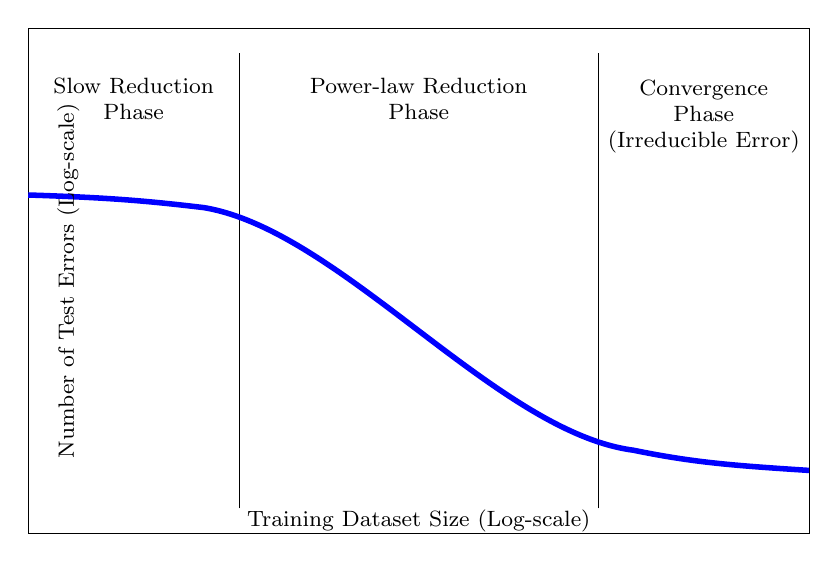
\begin{tikzpicture}

\def\upline{13.5}
\def\downline{2.5}
\def\upcenpos{17.2}

\begin{scope}
\begin{axis}[
width=11.5cm, height=8cm,
%symbolic x coords={1-15,16-25,26-35,>35},
%ytick={0,4,8,...,20},
%xtick={0,5,...,100},
xlabel={Training Dataset Size (Log-scale)},
ylabel={Number of Test Errors (Log-scale)},
xlabel style={align=center,yshift=1.2em,font=\footnotesize},
ylabel style={align=center,yshift=-2.2em,font=\footnotesize},
xticklabel style={fill=white,opacity=0},
yticklabel style={fill=white,opacity=0},
x tick style={fill=white,opacity=0},
y tick style={fill=white,opacity=0},
xtick=\empty,
ytick=\empty,
%x tick label style={font=\footnotesize},
%y tick label style={font=\footnotesize},
%tick align=inside,
%major grid style={draw=blue,dashed},
legend pos=outer north east,
%legend style={anchor=north west,yshift=-1cm},
%legend style={yshift=-4.5em,xshift=-6em,legend cell align=left,legend plot pos=right},
xmin=0,
xmax=100,
ymin=0,
ymax=20]
%\addplot [sharp plot,thick,blue] coordinates{(3,\upline) (22.5,13) (77.5, 3) (97, \downline)};

%\addplot [sharp plot,thick,blue,domain=2:23] (x,-0.00099*x*x+\upline-0.1);
%\addplot [sharp plot,thick,blue,domain=23:77] (x,-0.18*x+17.05);
%\addplot [sharp plot,thick,blue,domain=77:97] (x,0.001475*x^2 - 0.28615*x+13.878275+\downline+0.1);

\addplot [sharp plot] coordinates{(27,1) (27,19)};
\addplot [sharp plot] coordinates{(73,1) (73,19)};

%\addplot [sharp plot,very thick,dashed,green] coordinates{(2,\upline) (98,\upline)};
%\addplot [sharp plot,very thick,dashed,red] coordinates{(2,\downline) (98,\downline)};
{\footnotesize
\node[anchor=center,align=center,font=\footnotesize] (t1) at (axis cs:13.5,\upcenpos) {Slow Reduction\\ Phase};
\node[anchor=center,align=center,font=\footnotesize] (t2) at (axis cs:50,\upcenpos){Power-law Reduction\\ Phase};
\node[anchor=center, align=center,font=\footnotesize] (t3) at (axis cs:86.5,\upcenpos - 0.7) {Convergence \\ Phase \\ (Irreducible Error)};


%\draw[-,thick,purple] (axis cs:0,\upline-0.1) .. controls ([xshift=0em,yshift=0em]axis cs:0,\upline) and ([xshift=0em,yshift=-1em]axis cs:0,\upline) .. (axis cs:22.5,\upline-0.6);
\draw[-,line width=2pt,blue] (axis cs:0,\upline-0.1) .. controls ([xshift=0em,yshift=0em]axis cs:10,\upline-0.199) and ([xshift=0em,yshift=0em]axis cs:15,\upline-0.32275) .. (axis cs:22.5,\upline-0.6) .. controls ([xshift=0em,yshift=0em]axis cs:40,12) and ([xshift=0em,yshift=0em]axis cs:60,4) .. (axis cs:77.5,\downline+0.8) .. controls ([xshift=0em,yshift=0em]axis cs:85,\downline+0.32275) and ([xshift=0em,yshift=0em]axis cs:90,\downline+0.199) .. (axis cs:100,\downline);
}
%\addplot [sharp plot,very thick,orange,mark=*] coordinates{(1-15,17.5) (16-25,24) (26-35,25) (>35,27)};
%\legend{\tiny{NMT},\tiny{SPB},\tiny{HPB},\tiny{PBSY}}
\end{axis}
\end{scope}
\end{tikzpicture}

%---------------------------------------------------------------------

\caption{A scaling law of test error against a variable of interest (e.g., training dataset size)~\cite{hestness-etal:2017deep}. The curve of the scaling law can be divided into three phases. Initially, the test error decreases slowly when more training data is used, but this only lasts for a short period. In the second phase, the test error decreases drastically, and the curve becomes a power-law curve. After that, the error reduction slows down again in the third phase. Note that there are irreducible errors that cannot be eliminated, regardless of the amount of training data.}
\label{fig:scaling-power-law-curve}
\end{figure}

To understand how model performance scales with various factors involved in training, it is common to express model performance as a function of these factors. For example, in the simplest case, we can express the loss or error of an LLM as a function of a single variable of interest. However, there are no universal scaling laws that can describe this relationship. Instead, different functions are proposed to fit the learning curves of LLMs.

Let $x$ be the variable of interest (such as the number of model parameters) and $\mathcal{L}(x)$ be the loss of the model given $x$ (such as the cross-entropy loss on test data). The simplest form of $\mathcal{L}(x)$ is a power law
\begin{eqnarray}
\mathcal{L}(x) & = & ax^b,
\end{eqnarray}

\noindent where $a$ and $b$ are parameters that are estimated empirically. Despite its simplicity, this function has successfully interpreted the scaling behavior of language models and machine translation systems in terms of model size (denoted by $N$) and training dataset size (denoted by $D$)~\cite{gordon-etal:2021data,hestness-etal:2017deep}. For example,~\citet{kaplan-etal:2020scaling} found that the performance of their language model improves as a power law of either $N$ or $D$ after an initial transient period, and expressed these relationships using $\mathcal{L}(N) = \big( \frac{N}{8.8 \times 10^{13}} \big)^{-0.076}$ and $\mathcal{L}(D) = \big( \frac{D}{5.4 \times 10^{13}} \big)^{-0.095}$ (see Figure~\ref{fig:power-law-scaling-for-model-size-and-dataset-size}).

\begin{figure}[!t]
\centering
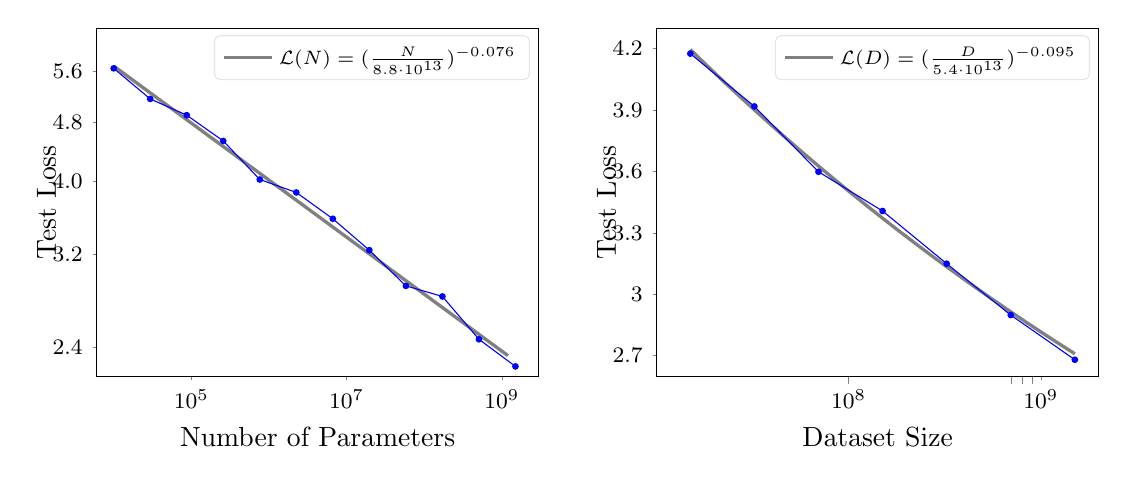
\begin{tikzpicture}

\pgfmathsetseed{765}

\begin{scope}
\begin{axis}[
width=7.2cm, height=6cm,
ytick={2.4,3.2,...,5.6},
yticklabels={$2.4$, $3.2$, $4.0$, $4.8$, $5.6$},
xtick={100000,10000000,1000000000},
xlabel={Number of Parameters},
ylabel={Test Loss},
xlabel style={align=center},
ylabel style={yshift=-0.8em},
x tick label style={font=\footnotesize},
y tick label style={font=\footnotesize},
tick align=outside,
tickpos=left,
major tick length=0.05cm,
xmode=log,
ymode=log,
legend style={font=\scriptsize,draw=gray!20,rounded corners=2pt},
xmin=6000,
xmax=3000000000,
ymin=2.2,
ymax=6.4]
\addplot [sharp plot,very thick,gray, domain=10000:1200000000] {(x/(8.8*10^13))^-0.076};
\legend{$\mathcal{L}(N)=(\frac{N}{8.8\cdot10^{13}})^{-0.076}$}

\addplot [sharp plot,blue,mark=*,mark size=1pt, samples=12, domain=10000:1500000000] {((x)/(8.8*10^13))^-0.076 + rand*0.1};
\end{axis}
\end{scope}

\pgfmathsetseed{265}

\begin{scope}[xshift=2.8in]
\begin{axis}[
width=7.2cm, height=6cm,
ytick={2.7,3.0,...,4.2},
xtick={100000000,1000000000},
xlabel={Dataset Size},
ylabel={Test Loss},
xlabel style={align=center},
ylabel style={yshift=-0.8em},
x tick label style={font=\footnotesize},
y tick label style={font=\footnotesize},
log identify minor tick positions=false,
tick align=outside,
tickpos=left,
major tick length=0.05cm,
xmode=log,
legend style={font=\scriptsize,draw=gray!20,rounded corners=2pt},
xmin=10000000,
xmax=2000000000,
ymin=2.6,
ymax=4.3]
\addplot [sharp plot,very thick,gray, domain=15000000:1500000000] {(x/(5.4*10^13))^-0.095};
\legend{$\mathcal{L}(D)=(\frac{D}{5.4\cdot10^{13}})^{-0.095}$}

\addplot [sharp plot,blue,mark=*,mark size=1pt, samples=7, domain=15000000:1500000000] {(x/(5.4*10^13))^-0.095 + rand*0.04};

\end{axis}
\node[anchor=north,fill=white,minimum width=5em,inner sep=0pt,minimum height=0.3em] (mask) at (10em,-0.02em) {};
\end{scope}

\end{tikzpicture}

%--------------------------------------------------------------------- 
\caption{Test loss against model size ($N$) and training dataset size ($D$) (data points are plotted for illustrative purposes). We plot test loss as a function of $N$, which is defined as $\mathcal{L}(N) = \big( \frac{N}{8.8 \times 10^{13}} \big)^{-0.076}$, and a function of $D$, which is defined as $\mathcal{L}(D) = \big( \frac{D}{5.4 \times 10^{13}} \big)^{-0.095}$ ~\cite{kaplan-etal:2020scaling}. }
\label{fig:power-law-scaling-for-model-size-and-dataset-size}
\end{figure}

An improvement to this scaling law is to add an \mindex{irreducible error} term to the power law. The form of $\mathcal{L}(x)$ is then given by

\begin{eqnarray}
\mathcal{L}(x) & = & ax^b + \epsilon_{\infty} \label{eq:scaling-laws-m2-form},
\end{eqnarray}

\noindent where $\epsilon_{\infty}$ is the irreducible error that accounts for the error due to unknown variables, which is present even as $x \to \infty$. Eq. (\ref{eq:scaling-laws-m2-form}) is one of the most widely used forms for modeling scaling laws of LLMs. For example,~\citet{rosenfeld-etal:2020constructive} developed a scaling law that involves both model scaling and dataset scaling, as follows
\begin{eqnarray}
\mathcal{L}(N,D) & = & aN^b + cD^d + \epsilon_{\infty}.
\end{eqnarray}

An example of such a formulation is the Chinchilla scaling law. It states that the test loss per token is the sum of the inverse power-law functions of $N$ and $D$, with an additional irreducible error term.~\citet{hoffmann-etal:2022training} express this scaling law as
\begin{eqnarray}
\mathcal{L}(N,D) & = & \underbrace{\frac{406.4}{N^{0.34}}}_{\textrm{model scaling}} + \underbrace{\frac{410.7}{D^{0.28}}}_{\textrm{dataset scaling}} + \underbrace{1.69}_{\textrm{irreducible error}}.
\end{eqnarray}

All the scaling laws mentioned above are based on monotonic functions. So they cannot cover functions with inflection points, such as double descent curves. In response, researchers have explored more sophisticated functions to fit the learning curves. Examples of such functions can be found in~\citet{alabdulmohsin-etal:2022revisiting} and~\citet{caballero-etal:2023broken}'s work.

The significance of scaling laws lies in providing directional guidance for LLM research: if we are still in the region of the power-law curve, using more resources to train larger models is a very promising direction. While this result compels large research groups and companies to invest heavily in computational resources to train larger models, which is very expensive, scaling laws continuously push the boundaries of AI forward. On the other hand, understanding scaling laws helps researchers make informed decisions when training LLMs. For example, given the computational resources at hand, the ultimate performance of an LLM can be estimated.

As a final note on scaling laws in this section, for LLMs, a lower test loss does not always imply better performance on all downstream tasks. To adapt LLMs, there are several steps, such as fine-tuning and prompting, that may influence the final results. Therefore, the scaling laws for different downstream tasks might vary in practice.

%----------------------------------------------------------------------------------------
% NEW SECTION
%----------------------------------------------------------------------------------------

\section{Long Sequence Modeling}
\label{sec:long-sequence-modeling}

\noindent We have already seen that, in large-scale training, more powerful language models can be developed by scaling up both data and computational resources. However, scaling can also occur along other dimensions. For instance, in many modern applications, LLMs often need to be adapted to process very long sequences. A common scenario involves pre-training an LLM on texts of standard length, and subsequently applying it to sequences that far exceed those seen during pre-training. Here, we use $\Pr(\mathbf{y}|\mathbf{x})$ to denote the conditional probability of generating text, where $\mathbf{x}$ is the context and $\mathbf{y}$ is the generated text. Broadly speaking, long sequence modeling problems can be categorized into three types:

\begin{itemize}
\item \vspace{0.5em} \textbf{Long-context text generation} (i.e., where $\mathbf{x}$ is a long sequence). For example, generating a short summary for a lengthy document.
\item \vspace{0.3em} \textbf{Long-text generation} (i.e., where $\mathbf{y}$ is a long sequence). For example, generating a comprehensive story based on a few keywords.
\item \vspace{0.3em} \textbf{Long-context and long-text generation} (i.e., where both $\mathbf{x}$ and $\mathbf{y}$ are long sequences). For example, generating a translation of a long document from Chinese to English.
\end{itemize}
\vspace{0.5em}

Recently, NLP researchers have been more interested in applying and evaluating LLMs on tasks where extremely long input texts are involved. Imagine an LLM that reads a C++ source file containing tens of thousands of lines, and outlines the functionality of the program corresponding to the source file. Such models, capable of handling extensive textual contexts, are typically called \mindex{long-context LLMs}. In this section we will restrict ourselves to long-context LLMs, but the methods discussed here can be applied to other problems.

For Transformers, dealing with long sequences is computationally expensive, as the computational cost of self-attention grows quadratically with the sequence length. This makes it infeasible to train and deploy such models for very long inputs. Two strands of research have tried to adapt Transformers to long-context language modeling.

\begin{itemize}
\item \vspace{0.5em} The first explores efficient training methods and model architectures to learn self-attention models from long-sequence data.
\item \vspace{0.3em} The other adapts pre-trained LLMs to handle long sequences with modest or no fine-tuning.
\end{itemize}
\vspace{0.5em}

Here, we will discuss the former briefly  since it can be found in general discussions of efficient Transformer architectures \cite{Tay-etal:2020efficient,xiao-and-zhu:2023introduction}. We will focus on the latter, highlighting popular methods in recent LLMs. We will also discuss the strengths and limitations of these long-sequence models.

\subsection{Hardware and Parallel Computing Optimizations}

\noindent We begin our discussion by considering improvements to standard Transformer models from the perspective of high-performance computing. Most of these improvements, though not specifically designed for LLMs, have been widely applied across various deep learning models~\cite{kim-etal:2023full}. A commonly used approach is to adopt reduced-precision data formats. For example, rather than using standard 32-bit floating-point (FP32) arithmetic, models can employ 16-bit floating-point (FP16/BF16) or even 8-bit integer (INT8) quantization. Using these low-precision data types can improve computational efficiency and memory throughput, so that longer sequences can be processed more easily. An alternative approach is to improve Transformers by using hardware-aware techniques. For example, on modern GPUs, the efficiency of Transformers can be improved by using IO-aware implementations of the self-attention function~\cite{dao-etal:2022flashattention,kwon-etal:2023efficient}.

Another way to handle long sequences is through sequence parallelism~\cite{li-etal:2023sequence,korthikanti-etal:2023reducing}. Specifically, consider the general problem of attending the query $\mathbf{q}_i$ at the position $i$ to the keys $\mathbf{K}$ and values $\mathbf{V}$. We can divide $\mathbf{K}$ along the sequence dimension (i.e., by rows) and obtain a set of sub-matrices $\{\mathbf{K}^{[1]},\cdots,\mathbf{K}^{[n_u]}\}$, each corresponding to a segment of the sequence. Similarly, we can obtain the sub-matrices of $\mathbf{V}$, denoted by $\{\mathbf{V}^{[1]},\cdots,\mathbf{V}^{[n_u]}\}$. Then, we assign each pair of $\mathbf{K}^{[u]}$ and $\mathbf{V}^{[u]}$ to a compute node (e.g., a GPU of a GPU cluster). The assigned nodes can run in parallel, thereby parallelizing the attention operation.

Recall that the output of the self-attention model can be written as
\begin{eqnarray}
\mathrm{Att}_{\mathrm{qkv}}(\mathbf{q}_i,\mathbf{K},\mathbf{V}) & = & \sum_{j=0}^{m-1} \alpha_{i,j} \mathbf{v}_j \label{eq:seq-parallel-qkv},
\end{eqnarray}

\noindent where $\alpha_{i,j}$ is the attention weight between positions $i$ and $j$. In Transformers, $\alpha_{i,j}$ is obtained by normalizing the scaled dot product between $\mathbf{q}_i$ and $\mathbf{k}_j$. Let $\beta_{i,j}$ denote the attention score between $\mathbf{q}_i$ and $\mathbf{k}_j$. We have
\begin{eqnarray}
\beta_{i,j} & = & \frac{\mathbf{q}_i \cdot \mathbf{k}_j}{\sqrt{d}}  + \mathrm{Mask}(i,j),
\end{eqnarray}

\noindent where $\mathrm{Mask}(i,j)$ is the causal mask value for the position pair $(i,j)$. Then, we define the attention weight $\alpha_{i,j}$ to be

\begin{eqnarray}
\alpha_{i,j} & = & \mathrm{Softmax}(\beta_{i,j}) \nonumber \\
             & = & \frac{\exp(\beta_{i,j})}{\sum_{j'} \exp(\beta_{i,j'})} \label{eq:seq-parallel-att-weight}.
\end{eqnarray}

On each compute node, we need to implement these equations. Given the keys and values assigned to this node, computing the numerator of the right-hand side of Eq. (\ref{eq:seq-parallel-att-weight}) (i.e., $\exp(\beta_{i,j})$) is straightforward, as all the required information is stored on the node. However, computing the denominator of the right-hand side of Eq. (\ref{eq:seq-parallel-att-weight}) involves a sum of $\exp(\beta_{i,j'})$ over all $j'$, which requires transferring data to and from other nodes. To illustrate, suppose that $\mathbf{v}_j$ and $\mathbf{k}_j$ are placed on node $u$. We can rewrite Eq. (\ref{eq:seq-parallel-att-weight}) as
\begin{eqnarray}
&   & \alpha_{i,j} \nonumber \\
& = & \frac{\overbrace{\exp(\beta_{i,j})}^{\textrm{node $u$}}}{\underbrace{\sum_{\mathbf{k}_{j'} \in \mathbf{K}^{[1]}} \exp(\beta_{i,j'}) }_{\textrm{node $1$}} + \cdots + \underbrace{\sum_{\mathbf{k}_{j'} \in \mathbf{K}^{[u]}} \exp(\beta_{i,j'}) }_{\textrm{node $u$}} + \cdots + \underbrace{\sum_{\mathbf{k}_{j'} \in \mathbf{K}^{[n_u]}} \exp(\beta_{i,j'}) }_{\textrm{node $n_u$}} } \label{eq:seq-parallel-att-weight-distributed},
\end{eqnarray}

\noindent where the notation $\mathbf{k}_{j'} \in \mathbf{K}^{[u]}$ indicates that $\mathbf{k}_{j'}$ is a row vector of $\mathbf{K}^{[u]}$. In a straightforward implementation, we first perform the summations $\{ \sum_{\mathbf{k}_{j'} \in \mathbf{K}^{[u]}} \exp(\beta_{i,j'}) \}$ separately on the corresponding nodes. Then, we collect these summation results from different nodes to combine them into a final result. This corresponds to a collective operation in the context of parallel processing. There are many efficient implementations of such operations, such as all-reduce operations. Hence the sum of all $\exp(\beta_{i,j})$ values can be computed using optimized routines in collective communication toolkits.

Given the attention weights $\{\alpha_{i,j}\}$, we then compute the attention results using Eq. (\ref{eq:seq-parallel-qkv}). The problem can be re-expressed as
\begin{eqnarray}
&   & \mathrm{Att}_{\mathrm{qkv}}(\mathbf{q}_i,\mathbf{K},\mathbf{V}) \nonumber \\
& = & \underbrace{\sum_{\mathbf{v}_{j'} \in \mathbf{V}^{[1]}} \alpha_{i,j'} \mathbf{v}_{j'} }_{\textrm{node $1$}} + \cdots + \underbrace{\sum_{\mathbf{v}_{j'} \in \mathbf{V}^{[u]}} \alpha_{i,j'} \mathbf{v}_{j'} }_{\textrm{node $u$}} + \cdots + \underbrace{\sum_{\mathbf{v}_{j'} \in \mathbf{V}^{[n_u]}} \alpha_{i,j'} \mathbf{v}_{j'} }_{\textrm{node $n_u$}} \label{eq:seq-parallel-qkv-distributed}.
\end{eqnarray}

Like Eq. (\ref{eq:seq-parallel-att-weight-distributed}), Eq. (\ref{eq:seq-parallel-qkv-distributed}) can be implemented as a reduction operation in parallel processing. First, we perform the weighted summations of values on different nodes simultaneously. Then, we collect the results from these nodes via collective operations.

Note that, although this section primarily focuses on long sequence modeling, much of the motivation for sequence parallelism comes from the distributed training methods of deep networks, as discussed in Section~\ref{sec:llm-distributed-training}. As a result, the implementation of these methods can be built on the same parallel processing library.

\subsection{Efficient Architectures}

\noindent One difficulty of applying Transformers to long sequences is that standard self-attention suffers from quadratic time and memory complexity with respect to the sequence length.  Moreover, autoregressive generation requires maintaining a \mindex{key-value cache} (or \mindex{KV cache}), whose size increases as more tokens are processed. Although the KV cache footprint grows linearly with sequence length, for extremely long contexts, this memory requirement becomes prohibitive, making standard LLM deployment impractical. As a result, the model architecture of long-context LLMs generally moves away from the standard Transformer, turning instead to the development of more efficient variants and alternatives.

One approach is to replace standard self-attention with sparse attention. This family of models is motivated by the observation that attention distributions in long sequences are often highly skewed. Thus, only a small subset of tokens significantly impacts the context of any given token. Consequently, we can prune the vast majority of attention weights, representing the mechanism in a highly compressed form. To illustrate, consider the standard self-attention formulation:
\begin{eqnarray}
\mathrm{Att}_{\mathrm{qkv}}(\mathbf{Q},\mathbf{K},\mathbf{V}) & = & \alpha(\mathbf{Q},\mathbf{K}) \mathbf{V} \label{eq:qkv-attention-attention-weights},
\end{eqnarray}

\noindent where the attention weight matrix $\alpha(\mathbf{Q},\mathbf{K}) \in \mathbb{R}^{m \times m}$ is obtained by
\begin{eqnarray}
\alpha(\mathbf{Q},\mathbf{K}) & = & \mathrm{Softmax}(\frac{\mathbf{Q} \mathbf{K}^\top}{\sqrt{d}} + \mathbf{Mask}) \nonumber \\
                              & = & \begin{bmatrix} \alpha_{0,0} & 0 & 0 & \cdots & 0 \\ \alpha_{1,0} & \alpha_{1,1} & 0 & \cdots & 0 \\ \alpha_{2,0} & \alpha_{2,1} & \alpha_{2,2} & \cdots & 0 \\ \vdots & \vdots & \vdots & \ddots & \vdots \\ \alpha_{m-1,0} & \alpha_{m-1,1} & \alpha_{m-1,2} & \cdots & \alpha_{m-1,m-1} \end{bmatrix}.
\end{eqnarray}

Each row vector $\begin{bmatrix} \alpha_{i,0} & \cdots & \alpha_{i,i} & 0 & \cdots & 0 \end{bmatrix}$ corresponds to a distribution over tokens indicating how the $i$-th token attends to others. Since language models predict the next token only based on their left-context, we normally write the output of the attention model at position $i$ as
\begin{eqnarray}
\mathrm{Att}_{\mathrm{qkv}}(\mathbf{q}_i,\mathbf{K}_{\le i},\mathbf{V}_{\le i}) & = & \begin{bmatrix} \alpha_{i,0} & \cdots & \alpha_{i,i}  \end{bmatrix} \begin{bmatrix} \mathbf{v}_0 \\ \vdots \\ \mathbf{v}_{i} \end{bmatrix} \nonumber \\
                                                                                & = & \sum_{j = 0}^{i} \alpha_{i,j} \mathbf{v}_{j},
\end{eqnarray}

\noindent where $\mathbf{K}_{\le i} = \begin{bmatrix} \mathbf{k}_0 \\ \vdots \\ \mathbf{k}_{i} \end{bmatrix}$ and $\mathbf{V}_{\le i} = \begin{bmatrix} \mathbf{v}_0 \\ \vdots \\ \mathbf{v}_{i} \end{bmatrix}$ are the keys and values up to position $i$.

In standard self-attention, the vector $\begin{bmatrix} \alpha_{i,0} & \cdots & \alpha_{i,i} \end{bmatrix}$ is assumed to be dense, meaning almost all valid entries are non-zero. In sparse attention, only a predefined subset of these entries is computed, while the remainder are explicitly ignored (forced to zero). Let $G \subseteq \{0,\cdots,i\}$ denote the index set of the active (non-zero) entries. The output of the sparse attention model at position $i$ then becomes:
\begin{eqnarray}
\mathrm{Att}_{\mathrm{sparse}}(\mathbf{q}_i,\mathbf{K}_{\le i},\mathbf{V}_{\le i}) & = & \sum_{j \in G} \alpha'_{i,j} \mathbf{v}_{j}.
\end{eqnarray}

\noindent Here $\{\alpha'_{i,j}\}$ are normalized over $G$. Hence their values are different from the original attention weights (in fact we have $\alpha'_{i,j} > \alpha_{i,j}$). The sparsity of the model is determined by the size of $G$. Sparse attention models differ in the way we define $G$. One simple approach is to define $G$ based on heuristically designed patterns. For example, a widely-used pattern involves having $G$ cover a window of tokens located near position $i$~\cite{parmar-etal:2018image}.

While sparse attention reduces the computation through the use of sparse operations, such models still have significant limitations as we need to keep the entire KV cache (i.e., $\mathbf{K}_{\le i}$ and $\mathbf{V}_{\le i}$) during inference. If the sequence is very long, storing this cache will become highly memory-intensive. To address this, we can consider a different class of attention models where the KV cache is not explicitly retained. Linear attention is one such approach~\cite{katharopoulos-etal:2020transformers}. It uses a kernel function $\phi(\cdot)$ to map each query and key into a feature space, yielding $\mathbf{q}'_i = \phi(\mathbf{q}_i)$ and $\mathbf{k}'_i = \phi(\mathbf{k}_i)$, respectively. By replacing the Softmax normalization with a linear formulation\footnote{In the new space after this transformation, the Softmax normalization can be transformed into the simple scaling normalization.}, the form of the resulting attention model is given by

\begin{eqnarray}
\mathrm{Att}_{\mathrm{qkv}}(\mathbf{q}_i,\mathbf{K}_{\le i},\mathbf{V}_{\le i}) & \approx & \mathrm{Att}_{\mathrm{linear}}(\mathbf{q}'_i,\mathbf{K}'_{\le i},\mathbf{V}_{\le i}) \nonumber \\
                                                                                & = & \frac{\mathbf{q}'_{i} \mu_i}{\mathbf{q}'_{i} \nu_i},
\end{eqnarray}

\noindent where $\mu_i$ and $\nu_i$ are variables that are computed in a recurrent manner

\begin{eqnarray}
\mu_i & = & \mu_{i-1} + {\mathbf{k}'}_{i}^\top \mathbf{v}_{i} \label{eq:linear-attention-mu-llm} \\
\nu_i & = & \nu_{i-1} + {\mathbf{k}'}_{i}^\top \label{eq:linear-attention-nu-llm}.
\end{eqnarray}

\noindent $\mu_i$ and $\nu_i$ can be seen as summaries of the history up to position $i$. A benefit of this model is that we do not need to explicitly store all past keys and values. Instead only the latest representations $\mu_i$ and $\nu_i$ are used. So the computational cost of each step is a constant, and the model can be easily extended to deal with long sequences.

In fact, this sequential approach to long sequence modeling arises naturally when we adopt the perspective of recurrent models. Such models read one token (or a small number of tokens) at a time, update the recurrent state using these inputs, and then discard them before the next token arrives. The output at each step is generated based only on the recurrent state, rather than on all the previous states. The memory footprint is determined by the recurrent state which has a fixed size. Recurrent models can be used in real-time learning scenarios where data arrives in a stream and predictions can be made at any time step. In NLP, applying recurrent models to language modeling is  one of the earliest successful attempts to learn representations of sequences. Although Transformers have been used as the foundational architecture in LLMs, recurrent models are still powerful models, especially for developing efficient LLMs. For example, recurrent models, particularly modern state space models like Mamba~\cite{gu-and-dao:2023mamba}, have seen a resurgence in language modeling and have been reconsidered as a promising alternative to Transformers.

Figure~\ref{fig:comparison-of-efficient-llm-architectures} shows a comparison of the models discussed in this subsection. Since these models, along with others not mentioned here, have been extensively discussed in related surveys~\cite{Tay-etal:2020efficient,xiao-and-zhu:2023introduction}, a more exhaustive discussion is omitted here.

\begin{figure}[!t]
\centering
% !Mode:: "TeX:UTF-8"
% !TEX encoding = UTF-8 Unicode

\begin{center}
\begin{tikzpicture}
	
\def\ssep{0.80cm}

\tikzstyle{snode} = [minimum width=1*\ssep,minimum height=1*\ssep,inner sep=0pt,draw,very thin];

%%% sub-figure 1: standard self-attention
\begin{scope}

\node [snode,anchor=west,draw,thick] (qi) at (0,0) {\normalsize{$\mathbf{q}_i$}};

\node [snode,anchor=east,fill=blue!30] (kim0) at ([xshift=-2*\ssep]qi.west) {\footnotesize{$\mathbf{k}_{i}$}};
\node [snode,anchor=east,fill=blue!30] (kim1) at ([xshift=-1*\ssep]kim0.west) {\footnotesize{$\mathbf{k}_{i-1}$}};
\node [snode,anchor=east,fill=blue!30] (kim2) at ([xshift=-1*\ssep]kim1.west) {\footnotesize{$\mathbf{k}_{i-2}$}};
\node [anchor=east] (kdots) at ([xshift=-0.7*\ssep]kim2.west) {\footnotesize{$\cdots$}};
\node [snode,anchor=east,fill=blue!30] (k1) at ([xshift=-0.7*\ssep]kdots.west) {\footnotesize{$\mathbf{k}_{1}$}};
\node [snode,anchor=east,fill=blue!30] (k0) at ([xshift=-1*\ssep]k1.west) {\footnotesize{$\mathbf{k}_{0}$}};

\node [snode,anchor=north,fill=blue!30] (vim0) at ([yshift=-0.1cm]kim0.south) {\footnotesize{$\mathbf{v}_{i}$}};
\node [snode,anchor=north,fill=blue!30] (vim1) at ([yshift=-0.1cm]kim1.south) {\footnotesize{$\mathbf{v}_{i-1}$}};
\node [snode,anchor=north,fill=blue!30] (vim2) at ([yshift=-0.1cm]kim2.south) {\footnotesize{$\mathbf{v}_{i-2}$}};
\node [anchor=east] (vdots) at ([xshift=-0.7*\ssep]vim2.west) {\footnotesize{$\cdots$}};
\node [snode,anchor=north,fill=blue!30] (v1) at ([yshift=-0.1cm]k1.south) {\footnotesize{$\mathbf{v}_{1}$}};
\node [snode,anchor=north,fill=blue!30] (v0) at ([yshift=-0.1cm]k0.south) {\footnotesize{$\mathbf{v}_{0}$}};

\draw [->] ([xshift=-0.4cm,yshift=0.1em]qi.north) .. controls +(north:0.2cm) and +(north:0.5cm) .. ([yshift=0.1em]kim0.north);
\draw [->] ([xshift=-0.3cm,yshift=0.1em]qi.north) .. controls +(north:0.5cm) and +(north:0.7cm) .. ([yshift=0.1em]kim1.north);
\draw [->] ([xshift=-0.2cm,yshift=0.1em]qi.north) .. controls +(north:0.8cm) and +(north:0.9cm) .. ([yshift=0.1em]kim2.north);
\draw [->] ([xshift=-0.1cm,yshift=0.1em]qi.north) .. controls +(north:1.1cm) and +(north:1.1cm) .. ([yshift=0.1em]k1.north);
\draw [->] ([xshift=-0.0cm,yshift=0.1em]qi.north) .. controls +(north:1.4cm) and +(north:1.3cm) .. ([yshift=0.1em]k0.north);

\node [anchor=south] (attention) at ([yshift=0.8cm,xshift=0.6cm]qi.north) {\small{$\mathrm{Att}_{\mathrm{qkv}}(\mathbf{q}_i,\mathbf{K}_{\le i},\mathbf{V}_{\le i})$}};

\node [anchor=north] (caption) at ([yshift=-0.4cm,xshift=-0.3cm]vim1.south) {\small{(a) Standard Self-attention}};

\end{scope}

%%% sub-figure 2: spase attention
\begin{scope}[yshift=-4.5cm]

\node [snode,anchor=west,draw,thick] (qi) at (0,0) {\normalsize{$\mathbf{q}_i$}};

\node [snode,anchor=east,fill=blue!30] (kim0) at ([xshift=-2*\ssep]qi.west) {\footnotesize{$\mathbf{k}_{i}$}};
\node [snode,anchor=east,fill=gray!20,dotted,draw=white] (kim1) at ([xshift=-1*\ssep]kim0.west) {\color{gray} \footnotesize{$\mathbf{k}_{i-1}$}};
\node [snode,anchor=east,fill=gray!20,dotted,draw=white] (kim2) at ([xshift=-1*\ssep]kim1.west) {\color{gray} \footnotesize{$\mathbf{k}_{i-2}$}};
\node [anchor=east] (kdots) at ([xshift=-0.7*\ssep]kim2.west) {\footnotesize{$\cdots$}};
\node [snode,anchor=east,fill=blue!30] (k1) at ([xshift=-0.7*\ssep]kdots.west) {\footnotesize{$\mathbf{k}_{1}$}};
\node [snode,anchor=east,fill=gray!20,dotted,draw=white] (k0) at ([xshift=-1*\ssep]k1.west) {\color{gray} \footnotesize{$\mathbf{k}_{0}$}};

\node [snode,anchor=north,fill=blue!30] (vim0) at ([yshift=-0.1cm]kim0.south) {\footnotesize{$\mathbf{v}_{i}$}};
\node [snode,anchor=north,fill=gray!20,dotted,draw=white] (vim1) at ([yshift=-0.1cm]kim1.south) {\color{gray} \footnotesize{$\mathbf{v}_{i-1}$}};
\node [snode,anchor=north,fill=gray!20,dotted,draw=white] (vim2) at ([yshift=-0.1cm]kim2.south) {\color{gray} \footnotesize{$\mathbf{v}_{i-2}$}};
\node [anchor=east] (vdots) at ([xshift=-0.7*\ssep]vim2.west) {\footnotesize{$\cdots$}};
\node [snode,anchor=north,fill=blue!30] (v1) at ([yshift=-0.1cm]k1.south) {\footnotesize{$\mathbf{v}_{1}$}};
\node [snode,anchor=north,fill=gray!20,dotted,draw=white] (v0) at ([yshift=-0.1cm]k0.south) {\color{gray} \footnotesize{$\mathbf{v}_{0}$}};

\draw [->] ([xshift=-0.4cm,yshift=0.1em]qi.north) .. controls +(north:0.2cm) and +(north:0.5cm) .. ([yshift=0.1em]kim0.north);
%\draw [->] ([xshift=-0.3cm,yshift=0.1em]qi.north) .. controls +(north:0.5cm) and +(north:0.7cm) .. ([yshift=0.1em]kim1.north);
%\draw [->] ([xshift=-0.2cm,yshift=0.1em]qi.north) .. controls +(north:0.8cm) and +(north:0.9cm) .. ([yshift=0.1em]kim2.north);
\draw [->] ([xshift=-0.1cm,yshift=0.1em]qi.north) .. controls +(north:1.1cm) and +(north:1.1cm) .. ([yshift=0.1em]k1.north);
%\draw [->] ([xshift=-0.0cm,yshift=0.1em]qi.north) .. controls +(north:1.4cm) and +(north:1.3cm) .. ([yshift=0.1em]k0.north);

\node [anchor=south] (attention) at ([yshift=0.8cm,xshift=0.0cm]qi.north) {\small{$\mathrm{Att}_{\mathrm{qkv}}(\mathbf{q}_i,\{\mathbf{k}_{1},\mathbf{k}_{i}\},\{\mathbf{v}_{1},\mathbf{v}_{i}\})$}};

\node [anchor=north] (caption) at ([yshift=-0.4cm,xshift=-0.3cm]vim1.south) {\small{(b) Sparse Attention}};

\end{scope}

%%% sub-figure 3: linear attention
\begin{scope}[yshift=-9.5cm]

\node [snode,anchor=west,draw,thick] (qi) at (0,0) {\normalsize{$\mathbf{q}_i$}};

\node [snode,anchor=east] (kim0) at ([xshift=-2*\ssep]qi.west) {\footnotesize{$\mathbf{k}_{i}$}};
\node [snode,anchor=east] (kim1) at ([xshift=-1*\ssep]kim0.west) {\footnotesize{$\mathbf{k}_{i-1}$}};
\node [snode,anchor=east] (kim2) at ([xshift=-1*\ssep]kim1.west) {\footnotesize{$\mathbf{k}_{i-2}$}};
\node [anchor=east] (kdots) at ([xshift=-0.7*\ssep]kim2.west) {\footnotesize{$\cdots$}};
\node [snode,anchor=east] (k1) at ([xshift=-0.7*\ssep]kdots.west) {\footnotesize{$\mathbf{k}_{1}$}};
\node [snode,anchor=east] (k0) at ([xshift=-1*\ssep]k1.west) {\footnotesize{$\mathbf{k}_{0}$}};

\node [snode,anchor=north] (vim0) at ([yshift=-0.1cm]kim0.south) {\footnotesize{$\mathbf{v}_{i}$}};
\node [snode,anchor=north] (vim1) at ([yshift=-0.1cm]kim1.south) {\footnotesize{$\mathbf{v}_{i-1}$}};
\node [snode,anchor=north] (vim2) at ([yshift=-0.1cm]kim2.south) {\footnotesize{$\mathbf{v}_{i-2}$}};
\node [anchor=east] (vdots) at ([xshift=-0.7*\ssep]vim2.west) {\footnotesize{$\cdots$}};
\node [snode,anchor=north] (v1) at ([yshift=-0.1cm]k1.south) {\footnotesize{$\mathbf{v}_{1}$}};
\node [snode,anchor=north] (v0) at ([yshift=-0.1cm]k0.south) {\footnotesize{$\mathbf{v}_{0}$}};

\draw [decoration={brace,amplitude=7pt},decorate] ([yshift=0.1cm]k0.north west) --  ([yshift=0.1cm]kim0.north east) node [pos=0.5,above,yshift=0.3cm] (nui) {\small{$\nu_i = \nu_{i-1} + \mathbf{k'}_{i}^{\mathrm{T}}$}};
\node [anchor=south west] (mui) at (nui.north west) {\small{$\mu_i = \mu_{i-1} + \mathbf{k'}_{i}^{\mathrm{T}} \mathbf{v}_{i}$}};

\node [snode,anchor=west,minimum width=0.6*\ssep,minimum height=0.6*\ssep,fill=blue!30] (nuibox) at ([xshift=1.5cm]nui.east) {\footnotesize{$\nu_i$}};
\node [snode,anchor=south,minimum width=0.6*\ssep,minimum height=0.6*\ssep,fill=blue!30] (muibox) at ([yshift=0.2cm]nuibox.north) {\footnotesize{$\mu_i$}};

\node [anchor=east] (muarrow) at ([xshift=-0.4cm]muibox.west) {\small{$\Rightarrow$}};
\node [anchor=east] (nuarrow) at ([xshift=-0.4cm]nuibox.west) {\small{$\Rightarrow$}};

\begin{pgfonlayer}{background}
\node [draw,dotted] [fit = (nuibox) (muibox)] (numubox) {};
\end{pgfonlayer}

\draw [->] ([xshift=-0.0cm,yshift=0.1em]qi.north) .. controls +(north:0.7cm) and +(east:1cm) .. ([yshift=0.3cm,xshift=2pt]numubox.south east);

\node [anchor=south] (attention) at ([yshift=0.8cm,xshift=-0.1cm]qi.north) {\small{$\mathrm{Att}_{\mathrm{linear}}(\mathbf{q}_i,\mathbf{K}_{\le i},\mathbf{V}_{\le i}) = \frac{\mathbf{q}'_{i} \mu_i}{\mathbf{q}'_{i} \nu_i}$}};

\node [anchor=north] (caption) at ([yshift=-0.4cm,xshift=-0.3cm]vim1.south) {\small{(c) Linear Attention}};

\end{scope}

%%% sub-figure 4: recurrent models
\begin{scope}[yshift=-13.5cm]

\node [snode,anchor=west,draw,thick] (qi) at (0,0) {\normalsize{$\mathbf{h}_i$}};

\node [snode,anchor=east,fill=blue!30] (kim0) at ([xshift=-2*\ssep]qi.west) {\footnotesize{$\mathbf{h}_{i-1}$}};
\node [snode,anchor=east] (kim1) at ([xshift=-1*\ssep]kim0.west) {\footnotesize{$\mathbf{h}_{i-2}$}};
\node [snode,anchor=east] (kim2) at ([xshift=-1*\ssep]kim1.west) {\footnotesize{$\mathbf{h}_{i-3}$}};
\node [anchor=east] (kdots) at ([xshift=-0.7*\ssep]kim2.west) {\footnotesize{$\cdots$}};
\node [snode,anchor=east] (k1) at ([xshift=-0.7*\ssep]kdots.west) {\footnotesize{$\mathbf{h}_{1}$}};
\node [snode,anchor=east] (k0) at ([xshift=-1*\ssep]k1.west) {\footnotesize{$\mathbf{h}_{0}$}};

\draw [->] ([xshift=-0.4*\ssep]k0.west) -- ([xshift=-1pt]k0.west);
\draw [->] ([xshift=1pt]k0.east) -- ([xshift=-1pt]k1.west);
\draw [->] ([xshift=1pt]k1.east) -- ([xshift=0.4*\ssep]k1.east);
\draw [->] ([xshift=-0.4*\ssep]kim2.west) -- ([xshift=-1pt]kim2.west);
\draw [->] ([xshift=1pt]kim2.east) -- ([xshift=-1pt]kim1.west);
\draw [->] ([xshift=1pt]kim1.east) -- ([xshift=-1pt]kim0.west);
\draw [->] ([xshift=1pt]kim0.east) -- ([xshift=-1pt]qi.west);

\draw [->] ([yshift=-0.4*\ssep]k0.south) -- ([yshift=-1pt]k0.south);
\draw [->] ([yshift=-0.4*\ssep]k1.south) -- ([yshift=-1pt]k1.south);
\draw [->] ([yshift=-0.4*\ssep]kim2.south) -- ([yshift=-1pt]kim2.south);
\draw [->] ([yshift=-0.4*\ssep]kim1.south) -- ([yshift=-1pt]kim1.south);
\draw [->] ([yshift=-0.4*\ssep]kim0.south) -- ([yshift=-1pt]kim0.south);
\draw [->] ([yshift=-0.4*\ssep]qi.south) -- ([yshift=-1pt]qi.south);

\node [anchor=north] (qinput) at ([yshift=-0.3cm]qi.south) {\small{$\mathbf{input}_i$}};

\node [anchor=south] (attention) at ([yshift=0.4cm,xshift=-0.1cm]qi.north) {\small{$\mathbf{h}_i = f(\mathbf{h}_{i-1},\mathbf{input}_i)$}};

\node [anchor=north] (caption) at ([yshift=-0.7cm,xshift=-0.3cm]kim1.south) {\small{(d) Recurrent Models}};

\end{scope}
	
\end{tikzpicture}
\end{center}

\caption{Illustrations of self-attention, sparse attention, linear attention and recurrent models. Blue boxes = cached states for producing the output at position $i$. $f(\cdot)$ = a recurrent cell.}
\label{fig:comparison-of-efficient-llm-architectures}
\end{figure}

\subsection{Cache and Memory}
\label{sec:long-context-cache-and-memory}

\noindent LLMs based on the standard Transformer architecture employ global (dense) attention mechanisms. During autoregressive inference, these models require storing the entire left-context to make predictions for future tokens. This requires a KV cache, where the representations (i.e., keys and values) of all previously generated tokens are retained. As a result, the memory footprint of this cache grows linearly as inference proceeds. In the preceding sections, we discussed methods for mitigating this context bottleneck via efficient attention algorithms, such as sparse and linear attention. A related alternative approach is to explicitly encode and compress the context via an auxiliary memory module.

\subsubsection{Fixed-size KV Cache}

A straightforward approach is to represent the keys and values using a fixed-size memory model. Suppose we have a memory $\mathrm{Mem}$ which retains the contextual information. We can write the attention operation at position $i$ in a general form
\begin{eqnarray}
\mathrm{Att}(\mathbf{q}_i,\mathrm{Mem}) & = & \mathrm{Att}_{\mathrm{qkv}}(\mathbf{q}_i,\mathbf{K}_{\le i},\mathbf{V}_{\le i}).
\end{eqnarray}

In this model, $\mathrm{Mem}$ is simply the KV cache, i.e., $\mathrm{Mem} = (\mathbf{K}_{\le i}, \mathbf{V}_{\le i})$. Thus the size of $\mathrm{Mem}$ is determined by $i$. If $\mathrm{Mem}$ is defined to have a fixed size, then the cost of performing $\mathrm{Att}(\mathbf{q}_i,\mathrm{Mem})$ will be fixed. There are several alternative ways to design $\mathrm{Mem}$.

\begin{itemize}
\item \vspace{0.5em} One of the simplest methods is to consider a fixed-size window of previous keys and values. $\mathrm{Mem}$ is therefore given by
    \begin{eqnarray}
    \mathrm{Mem} & = & (\mathbf{K}_{[i - n_c + 1,i]},\mathbf{V}_{[i - n_c + 1,i]}),
    \end{eqnarray}
    \noindent where $n_c$ denotes the size of the window. The notation $\mathbf{K}_{[i - n_c + 1,i]}$ and $\mathbf{V}_{[i - n_c + 1,i]}$ denote the keys and values over positions from $i-n_c+1$ to $i$.\footnote{More formally, we write $\mathbf{K}_{[i - n_c + 1,i]} = \begin{bmatrix} \mathbf{k}_{i - n_c + 1} \\ \vdots \\ \mathbf{k}_{i} \end{bmatrix}$ and $\mathbf{V}_{[i - n_c + 1,i]} = \begin{bmatrix} \mathbf{v}_{i - n_c + 1} \\ \vdots \\ \mathbf{v}_{i} \end{bmatrix}$. Sometimes we denote $\mathbf{K}_{[i - n_c + 1,i]}$ by $\{\mathbf{k}_{i - n_c + 1},\cdots,\mathbf{k}_{i}\}$ and $\mathbf{V}_{[i - n_c + 1,i]}$ by $\{\mathbf{v}_{i - n_c + 1},\cdots,\mathbf{v}_{i}\}$ for notational simplicity.} This model can be seen as a type of local attention model.
\item \vspace{0.5em} It is also possible to define $\mathrm{Mem}$ as a pair of summary vectors, which leads to a more compressed representation of the history. A simple way to summarize the previous keys and values is to use the moving averages of these vectors. For example, $\mathrm{Mem}$ can be defined as the unweighted moving average of the previous $n_c$ keys and values
    \begin{eqnarray}
    \mathrm{Mem} & = & \left(\frac{\sum_{j=i - n_c + 1}^{i} \mathbf{k}_{j}}{n_c} , \frac{\sum_{j=i - n_c + 1}^{i} \mathbf{v}_{j}}{n_c} \right).
    \end{eqnarray}

    Alternatively, we can use a weighted moving average
    \begin{eqnarray}
    \mathrm{Mem} & = & \left( \frac{\sum_{j=i - n_c + 1}^{i} \beta_{j - i + n_c} \mathbf{k}_{j}} {\sum_{j=1}^{n_c} \beta_j} , \frac{\sum_{j=i - n_c + 1}^{i} \beta_{j - i + n_c} \mathbf{v}_{j}}{\sum_{j=1}^{n_c} \beta_j} \right).
    \end{eqnarray}

    \noindent Here $\{\beta_1,\cdots,\beta_{n_c}\}$ are the coefficients, which can either be learned as model parameters or determined via heuristics. For example, they can be set to increasing coefficients (i.e., $\beta_{1} < \beta_{2} < \cdots < \beta_{n_c -1} < \beta_{n_c}$) in order to give larger weight to positions that are closer to $i$. We can extend the moving average to include all the positions up to $i$. This leads to the cumulative average of the keys and values, given in the form
    \begin{eqnarray}
    \mathrm{Mem} & = & \left( \frac{\sum_{j=0}^{i} \mathbf{k}_j}{i+1}, \frac{\sum_{j=0}^{i} \mathbf{v}_j}{i+1} \right).
    \end{eqnarray}

    In general, the cumulative average can be written in recursive form
    \begin{eqnarray}
    \mathrm{Mem}_{i} & = & \frac{(\mathbf{k}_i,\mathbf{v}_i) + i \cdot \mathrm{Mem}_{i-1}}{i + 1},
    \end{eqnarray}

    \noindent where $\mathrm{Mem}_{i}$ and $\mathrm{Mem}_{i-1}$ denote the cumulative averages of the current and previous positions, respectively. An advantage of this model is that we only need to store a single key-value pair during inference, rather than storing all the key-value pairs. Note that the above memory models are related to recurrent models, and more advanced techniques have been used to develop alternatives to self-attention mechanisms in Transformers~\cite{ma-etal:2023mega}.

\item \vspace{0.3em} The memory $\mathrm{Mem}$ can also be a neural network. At each step, it takes both the previous output of the memory and the current states of the model as input, and produces the new output of the memory. This neural network can be formulated as the function
    \begin{eqnarray}
    \mathrm{Mem} & = & \mathrm{Update}(S_{\mathrm{kv}}, \mathrm{Mem}_{\mathrm{pre}}) \label{eq:long-seq-mem-update}.
    \end{eqnarray}
    \noindent Here $\mathrm{Mem}$ and $\mathrm{Mem}_{\mathrm{pre}}$ represent the outputs of the memory at the current step and the previous step, respectively. $S_{\mathrm{kv}}$ is a set of key-value pairs, representing the recent states of the model. This formulation is general and allows us to develop various memory models by selecting different $\mathrm{Update}(\cdot)$ and $S_{\mathrm{kv}}$ configurations. For example, if $S_{\mathrm{kv}}$ only contains the latest key-value pair $(\mathbf{k}_i,\mathbf{v}_i)$ and $\mathrm{Update}(\cdot)$ is defined as a recurrent cell, then Eq. (\ref{eq:long-seq-mem-update}) can be expressed as an RNN-like model
    \begin{eqnarray}
    \mathrm{Mem} & = & f((\mathbf{k}_i,\mathbf{v}_i), \mathrm{Mem}_{\mathrm{pre}}),
    \end{eqnarray}

    \noindent where $f(\cdot)$ is a recurrent cell. Recurrence can also be applied to segment-level modeling for efficiency considerations. A simple approach is to divide the sequence into segments, and treat $S_{\mathrm{kv}}$ as a segment. Applying recurrent models to $\mathrm{Update}(\cdot)$ will result in memory models that operate on segments. A special case is to define $\mathrm{Update}(\cdot)$ as an FIFO function that adds $S_{\mathrm{kv}}$ into the memory and removes the oldest key-value segment from the memory, given by
    \begin{eqnarray}
    \mathrm{Mem} & = & \mathrm{FIFO}(S_{\mathrm{kv}}, \mathrm{Mem}_{\mathrm{pre}}).
    \end{eqnarray}

    \noindent Consider a memory which includes two segments, one for current segment, and one for the previous segment. In the attention operation, each position can access the history key-value pairs in the two most recent consecutive segments. While conceptually simple, this sliding-chunk local memory and its variants have been widely adopted in segment-level recurrent architectures~\cite{dai-etal:2019transformer,hutchins-etal:2022block,bulatov-etal:2022recurrent}.

\item \vspace{0.3em} The above memory models can be extended to involve multiple memories. An example of this approach is compressive Transformer~\cite{rae-etal:2020:compressive}. It employs two distinct fixed-size memories: one for modeling local context (denoted by $\mathrm{Mem}$), and the other for modeling and compressing long-term history (denoted by $\mathrm{CMem}$). The KV cache in this model is the combination of $\mathrm{Mem}$ and $\mathrm{CMem}$. The attention function can be written as
    \begin{eqnarray}
    \mathrm{Att}_{\mathrm{com}}(\mathbf{q}_i,\mathrm{Mem},\mathrm{CMem}) & = & \mathrm{Att}_{\mathrm{qkv}}(\mathbf{q}_i, [\mathrm{Mem},\mathrm{CMem}]),
    \end{eqnarray}

    \noindent where $[\mathrm{Mem},\mathrm{CMem}]$ is a combined memory of $\mathrm{Mem}$ and $\mathrm{CMem}$. Similar to standard segment-level models, the compressive Transformer processes the sequence in blocks. Each segment comprises $n_s$ consecutive tokens, and $S_{\mathrm{kv}}^{k}$ denotes the raw key-value pairs generated from the $k$-th segment. Upon the arrival of a new segment, $\mathrm{Mem}$ is updated via a FIFO queue: it appends the $n_s$ new key-value pairs from $S_{\mathrm{kv}}^{k}$ and simultaneously removes the $n_s$ oldest pairs:
    \begin{eqnarray}
    \mathrm{Mem} & = & \mathrm{FIFO}(S_{\mathrm{kv}}^{k}, \mathrm{Mem}_{\mathrm{pre}}).
    \end{eqnarray}

    \noindent Rather than discarding these ejected pairs, they are passed through a compression network. The $n_s$ raw pairs are compressed into a smaller set of $\frac{n_s}{c}$ condensed key-value pairs. Then $\mathrm{CMem}$ serves as a secondary FIFO queue, appending these $\frac{n_s}{c}$ compressed pairs and discarding its oldest $\frac{n_s}{c}$ entries to maintain fixed size. It is given by
    \begin{eqnarray}
    \mathrm{CMem}& = & \mathrm{FIFO}(C_{\mathrm{kv}}^{k}, \mathrm{CMem}_{\mathrm{pre}}),
    \end{eqnarray}

    \noindent where $C_{\mathrm{kv}}^{k}$ represents the set of compressed key-value pairs. The compressive Transformer implicitly assumes that local context should be represented explicitly with minimal  information loss, while long-range context can be more compressed.

\item \vspace{0.3em} We have already seen that both global and local contexts are useful and can be modeled using attention models. This view motivates the extension to attention models for combining both local and long-term memories~\cite{ainslie-etal:2020etc,zaheer-etal:2020big,gupta-berant:2020gmat}. A simple but widely-used approach is to involve the first few tokens of the sequence in attention, which serves as global tokens. This approach is usually applied along with other sparse attention models. An advantage of incorporating global tokens is that it serves as an attention sink that absorbs excessive attention scores, and thus stabilizes model performance when the context size is very large~\cite{xiao-etal:2024efficient}. One drawback, however, is that using a fixed-size global memory may result in information loss. When dealing with long sequences, we need to enlarge the KV cache for sufficient representations of the context, but this in turn increases the computational cost.

\end{itemize}
\vspace{0.5em}

Figure~\ref{fig:comparison-kv-cache-optimizations} shows illustrations of the above approaches. Note that, while we focus on optimization of the KV cache here, this issue is closely related to those discussed in the previous section. All of the methods we have mentioned so far can broadly be categorized as efficient attention approaches, which are widely used in various Transformer variants.

\begin{figure}[!t]
\centering
% !Mode:: "TeX:UTF-8"
% !TEX encoding = UTF-8 Unicode

\begin{center}
\begin{tikzpicture}
	
\def\ssep{0.50cm}

\tikzstyle{snode} = [minimum width=1*\ssep,minimum height=1*\ssep,inner sep=0pt,draw=blue,thick,fill=blue!30];
\tikzstyle{mnode} = [snode,draw=ugreen,fill=ugreen!30];

%%% sub-figure 1: window-based caching
\begin{scope}

\node [snode,anchor=east] (k1) at (0,0) {};
\node [snode,anchor=east] (k2) at ([xshift=-1*\ssep]k1.west) {};
\node [snode,anchor=east] (k3) at ([xshift=-1*\ssep]k2.west) {};
\node [snode,anchor=east] (k4) at ([xshift=-1*\ssep]k3.west) {};
\node [snode,anchor=east] (k5) at ([xshift=-1*\ssep]k4.west) {};
\node [snode,anchor=east] (k6) at ([xshift=-1*\ssep]k5.west) {};
\node [snode,anchor=east] (k7) at ([xshift=-1*\ssep]k6.west) {};
\node [snode,anchor=east] (k8) at ([xshift=-1*\ssep]k7.west) {};
\node [anchor=east] (kdots) at ([xshift=-1*\ssep]k8.west) {\small{$\cdots$}};

\node [snode,anchor=north] (v1) at ([yshift=-0.1cm]k1.south) {};
\node [snode,anchor=north] (v2) at ([yshift=-0.1cm]k2.south) {};
\node [snode,anchor=north] (v3) at ([yshift=-0.1cm]k3.south) {};
\node [snode,anchor=north] (v4) at ([yshift=-0.1cm]k4.south) {};
\node [snode,anchor=north] (v5) at ([yshift=-0.1cm]k5.south) {};
\node [snode,anchor=north] (v6) at ([yshift=-0.1cm]k6.south) {};
\node [snode,anchor=north] (v7) at ([yshift=-0.1cm]k7.south) {};
\node [snode,anchor=north] (v8) at ([yshift=-0.1cm]k8.south) {};
\node [anchor=east] (vdots) at ([xshift=-1*\ssep]v8.west) {\small{$\cdots$}};

\node [anchor=north] (p1) at ([yshift=-0.1cm]v1.south) {\scriptsize{$i$}};
\node [anchor=north] (p2) at ([yshift=-0.1cm]v2.south) {\scriptsize{$i-1$}};
\node [anchor=north] (p3) at ([yshift=-0.1cm]v3.south) {\scriptsize{$i-2$}};
\node [anchor=north] (p4) at ([yshift=-0.1cm]v4.south) {\scriptsize{$i-3$}};
\node [anchor=north] (p5) at ([yshift=-0.1cm]v5.south) {\scriptsize{$i-4$}};
\node [anchor=north] (p6) at ([yshift=-0.1cm]v6.south) {\scriptsize{$i-5$}};
\node [anchor=north] (p7) at ([yshift=-0.1cm]v7.south) {\scriptsize{$i-6$}};
\node [anchor=north] (p8) at ([yshift=-0.1cm]v8.south) {\scriptsize{$i-7$}};

\node [anchor=west] (keylabel) at ([xshift=0.3cm]k1.east) {\footnotesize{Keys}};
\node [anchor=west] (valuelabel) at ([xshift=0.3cm]v1.east) {\footnotesize{Values}};

\draw [decoration={brace,amplitude=4pt},decorate] ([yshift=0.1cm]k4.north west) --  ([yshift=0.1cm]k1.north east);

\node [mnode,anchor=south] (cv1) at ([yshift=0.6cm]k1.north) {};
\node [mnode,anchor=south] (cv2) at ([yshift=0.6cm]k2.north) {};
\node [mnode,anchor=south] (cv3) at ([yshift=0.6cm]k3.north) {};
\node [mnode,anchor=south] (cv4) at ([yshift=0.6cm]k4.north) {};

\node [mnode,anchor=south] (ck1) at ([yshift=0.1cm]cv1.north) {};
\node [mnode,anchor=south] (ck2) at ([yshift=0.1cm]cv2.north) {};
\node [mnode,anchor=south] (ck3) at ([yshift=0.1cm]cv3.north) {};
\node [mnode,anchor=south] (ck4) at ([yshift=0.1cm]cv4.north) {};

\begin{pgfonlayer}{background}
\node [draw,dotted,thick] [fit = (cv1) (ck4)] (membox) {};
\end{pgfonlayer}

\node [anchor=west] (sizelabel) at ([xshift=0.2cm]membox.east) {\small{$\textrm{Size} = 4 \times 2$}};
\node [anchor=south west] (memlabel) at ([yshift=-0.1cm]sizelabel.north west) {\small{Memory}};

\node [anchor=north] (caption) at ([yshift=-0.6cm]v4.south east) {\small{(a) Window-based Cache}};

\end{scope}

%%% sub-figure 2: moving average-based caching
\begin{scope}[yshift=-4.5cm]

\node [snode,anchor=east] (k1) at (0,0) {};
\node [snode,anchor=east] (k2) at ([xshift=-1*\ssep]k1.west) {};
\node [snode,anchor=east] (k3) at ([xshift=-1*\ssep]k2.west) {};
\node [snode,anchor=east] (k4) at ([xshift=-1*\ssep]k3.west) {};
\node [snode,anchor=east] (k5) at ([xshift=-1*\ssep]k4.west) {};
\node [snode,anchor=east] (k6) at ([xshift=-1*\ssep]k5.west) {};
\node [snode,anchor=east] (k7) at ([xshift=-1*\ssep]k6.west) {};
\node [snode,anchor=east] (k8) at ([xshift=-1*\ssep]k7.west) {};
\node [anchor=east] (kdots) at ([xshift=-1*\ssep]k8.west) {\small{$\cdots$}};

\node [snode,anchor=north] (v1) at ([yshift=-0.1cm]k1.south) {};
\node [snode,anchor=north] (v2) at ([yshift=-0.1cm]k2.south) {};
\node [snode,anchor=north] (v3) at ([yshift=-0.1cm]k3.south) {};
\node [snode,anchor=north] (v4) at ([yshift=-0.1cm]k4.south) {};
\node [snode,anchor=north] (v5) at ([yshift=-0.1cm]k5.south) {};
\node [snode,anchor=north] (v6) at ([yshift=-0.1cm]k6.south) {};
\node [snode,anchor=north] (v7) at ([yshift=-0.1cm]k7.south) {};
\node [snode,anchor=north] (v8) at ([yshift=-0.1cm]k8.south) {};
\node [anchor=east] (vdots) at ([xshift=-1*\ssep]v8.west) {\small{$\cdots$}};

\node [anchor=north] (p1) at ([yshift=-0.1cm]v1.south) {\scriptsize{$i$}};
\node [anchor=north] (p2) at ([yshift=-0.1cm]v2.south) {\scriptsize{$i-1$}};
\node [anchor=north] (p3) at ([yshift=-0.1cm]v3.south) {\scriptsize{$i-2$}};
\node [anchor=north] (p4) at ([yshift=-0.1cm]v4.south) {\scriptsize{$i-3$}};
\node [anchor=north] (p5) at ([yshift=-0.1cm]v5.south) {\scriptsize{$i-4$}};
\node [anchor=north] (p6) at ([yshift=-0.1cm]v6.south) {\scriptsize{$i-5$}};
\node [anchor=north] (p7) at ([yshift=-0.1cm]v7.south) {\scriptsize{$i-6$}};
\node [anchor=north] (p8) at ([yshift=-0.1cm]v8.south) {\scriptsize{$i-7$}};

\node [anchor=west] (keylabel) at ([xshift=0.3cm]k1.east) {\footnotesize{Keys}};
\node [anchor=west] (valuelabel) at ([xshift=0.3cm]v1.east) {\footnotesize{Values}};

\draw [decoration={brace,amplitude=4pt},decorate] ([yshift=0.1cm]k4.north west) --  ([yshift=0.1cm]k1.north east);

\node [mnode,anchor=south] (cv1) at ([yshift=0.6cm,xshift=1*\ssep]k3.north) {};

\node [mnode,anchor=south] (ck1) at ([yshift=0.1cm]cv1.north) {};

\begin{pgfonlayer}{background}
\node [draw,dotted,thick] [fit = (cv1) (ck1)] (membox) {};
\end{pgfonlayer}

\node [anchor=west] (sizelabel) at ([xshift=0.2cm]membox.east) {\small{$\textrm{Size} = 1 \times 2$}};
\node [anchor=south west] (memlabel) at ([yshift=-0.1cm]sizelabel.north west) {\small{Memory}};

\node [anchor=east] (keysaverage) at ([xshift=-0.4cm]ck1.west) {\footnotesize{$\frac{\mathbf{k}_{i-3} + \mathbf{k}_{i-2} + \mathbf{k}_{i-1} + \mathbf{k}_{i}}{4}\ \ \ \Rightarrow$}};
\node [anchor=east] (valuesaverage) at ([xshift=-0.4cm]cv1.west) {\footnotesize{$\frac{\mathbf{v}_{i-3} + \mathbf{v}_{i-2} + \mathbf{v}_{i-1} + \mathbf{v}_{i}}{4}\ \ \ \Rightarrow$}};

\node [anchor=north] (caption) at ([yshift=-0.6cm]v4.south east) {\small{(b) Moving Average-based Cache}};

\end{scope}

%%% sub-figure 3: recurrent networks as caches
\begin{scope}[yshift=-9cm]

\node [snode,anchor=east,fill=red!20,draw=red] (k1) at (0,0) {};
\node [snode,anchor=east] (k2) at ([xshift=-1*\ssep]k1.west) {};
\node [snode,anchor=east] (k3) at ([xshift=-1*\ssep]k2.west) {};
\node [snode,anchor=east] (k4) at ([xshift=-1*\ssep]k3.west) {};
\node [snode,anchor=east] (k5) at ([xshift=-1*\ssep]k4.west) {};
\node [snode,anchor=east] (k6) at ([xshift=-1*\ssep]k5.west) {};
\node [snode,anchor=east] (k7) at ([xshift=-1*\ssep]k6.west) {};
\node [snode,anchor=east] (k8) at ([xshift=-1*\ssep]k7.west) {};
\node [anchor=east] (kdots) at ([xshift=-1*\ssep]k8.west) {\small{$\cdots$}};

\node [snode,anchor=north,fill=red!20,draw=red] (v1) at ([yshift=-0.1cm]k1.south) {};
\node [snode,anchor=north] (v2) at ([yshift=-0.1cm]k2.south) {};
\node [snode,anchor=north] (v3) at ([yshift=-0.1cm]k3.south) {};
\node [snode,anchor=north] (v4) at ([yshift=-0.1cm]k4.south) {};
\node [snode,anchor=north] (v5) at ([yshift=-0.1cm]k5.south) {};
\node [snode,anchor=north] (v6) at ([yshift=-0.1cm]k6.south) {};
\node [snode,anchor=north] (v7) at ([yshift=-0.1cm]k7.south) {};
\node [snode,anchor=north] (v8) at ([yshift=-0.1cm]k8.south) {};
\node [anchor=east] (vdots) at ([xshift=-1*\ssep]v8.west) {\small{$\cdots$}};

\node [anchor=north] (p1) at ([yshift=-0.1cm]v1.south) {\scriptsize{$i$}};
\node [anchor=north] (p2) at ([yshift=-0.1cm]v2.south) {\scriptsize{$i-1$}};
\node [anchor=north] (p3) at ([yshift=-0.1cm]v3.south) {\scriptsize{$i-2$}};
\node [anchor=north] (p4) at ([yshift=-0.1cm]v4.south) {\scriptsize{$i-3$}};
\node [anchor=north] (p5) at ([yshift=-0.1cm]v5.south) {\scriptsize{$i-4$}};
\node [anchor=north] (p6) at ([yshift=-0.1cm]v6.south) {\scriptsize{$i-5$}};
\node [anchor=north] (p7) at ([yshift=-0.1cm]v7.south) {\scriptsize{$i-6$}};
\node [anchor=north] (p8) at ([yshift=-0.1cm]v8.south) {\scriptsize{$i-7$}};

\node [anchor=west] (keylabel) at ([xshift=0.3cm]k1.east) {\footnotesize{Keys}};
\node [anchor=west] (valuelabel) at ([xshift=0.3cm]v1.east) {\footnotesize{Values}};

\node [mnode,anchor=south] (cv1) at ([yshift=0.6cm]k1.north) {};

\node [mnode,anchor=south] (ck1) at ([yshift=0.1cm]cv1.north) {};

\begin{pgfonlayer}{background}
\node [draw,dotted,thick] [fit = (cv1) (ck1)] (membox) {};
\node [draw,dotted,thick] [fit = (v1) (k1)] (statebox) {};
\end{pgfonlayer}

\node [anchor=west] (sizelabel) at ([xshift=0.2cm]membox.east) {\small{$\textrm{Size} = 1 \times 2$}};
\node [anchor=south west] (memlabel) at ([yshift=-0.1cm]sizelabel.north west) {\small{Memory}};

\node [anchor=east] (eq) at ([xshift=-0.5cm]ck1.west) {\small{$\mathrm{Mem} = \mathrm{Update}($\colorbox{red!20}{$S_{\mathrm{kv}}$}$, \mathrm{Mem}_{\mathrm{pre}})\ \ \ \Rightarrow$}};

\draw [->] ([xshift=-0.0cm,yshift=-0.1em]statebox.north west) .. controls +(west:1cm) and +(south:1cm) .. ([yshift=0.1cm,xshift=0.1cm]eq.south);

\node [anchor=north] (caption) at ([yshift=-0.6cm]v4.south east) {\small{(c) Recurrent Network as Cache}};

\end{scope}

%%% sub-figure 4: hybrid cache
\begin{scope}[yshift=-14cm]

\node [snode,anchor=east] (k1) at (0,0) {};
\node [snode,anchor=east] (k2) at ([xshift=-1*\ssep]k1.west) {};
\node [snode,anchor=east] (k3) at ([xshift=-1*\ssep]k2.west) {};
\node [snode,anchor=east] (k4) at ([xshift=-1*\ssep]k3.west) {};
\node [snode,anchor=east] (k5) at ([xshift=-1*\ssep]k4.west) {};
\node [snode,anchor=east] (k6) at ([xshift=-1*\ssep]k5.west) {};
\node [snode,anchor=east] (k7) at ([xshift=-1*\ssep]k6.west) {};
\node [snode,anchor=east] (k8) at ([xshift=-1*\ssep]k7.west) {};
\node [anchor=east] (kdots) at ([xshift=-1*\ssep]k8.west) {\small{$\cdots$}};

\node [snode,anchor=north] (v1) at ([yshift=-0.1cm]k1.south) {};
\node [snode,anchor=north] (v2) at ([yshift=-0.1cm]k2.south) {};
\node [snode,anchor=north] (v3) at ([yshift=-0.1cm]k3.south) {};
\node [snode,anchor=north] (v4) at ([yshift=-0.1cm]k4.south) {};
\node [snode,anchor=north] (v5) at ([yshift=-0.1cm]k5.south) {};
\node [snode,anchor=north] (v6) at ([yshift=-0.1cm]k6.south) {};
\node [snode,anchor=north] (v7) at ([yshift=-0.1cm]k7.south) {};
\node [snode,anchor=north] (v8) at ([yshift=-0.1cm]k8.south) {};
\node [anchor=east] (vdots) at ([xshift=-1*\ssep]v8.west) {\small{$\cdots$}};

\node [anchor=north] (p1) at ([yshift=-0.1cm]v1.south) {\scriptsize{$i$}};
\node [anchor=north] (p2) at ([yshift=-0.1cm]v2.south) {\scriptsize{$i-1$}};
\node [anchor=north] (p3) at ([yshift=-0.1cm]v3.south) {\scriptsize{$i-2$}};
\node [anchor=north] (p4) at ([yshift=-0.1cm]v4.south) {\scriptsize{$i-3$}};
\node [anchor=north] (p5) at ([yshift=-0.1cm]v5.south) {\scriptsize{$i-4$}};
\node [anchor=north] (p6) at ([yshift=-0.1cm]v6.south) {\scriptsize{$i-5$}};
\node [anchor=north] (p7) at ([yshift=-0.1cm]v7.south) {\scriptsize{$i-6$}};
\node [anchor=north] (p8) at ([yshift=-0.1cm]v8.south) {\scriptsize{$i-7$}};

\node [anchor=west] (keylabel) at ([xshift=0.3cm]k1.east) {\footnotesize{Keys}};
\node [anchor=west] (valuelabel) at ([xshift=0.3cm]v1.east) {\footnotesize{Values}};

\node [mnode,anchor=south] (cv1) at ([yshift=0.6cm]k1.north) {};
\node [mnode,anchor=south] (cv2) at ([yshift=0.6cm]k2.north) {};
\node [mnode,anchor=south] (cv3) at ([yshift=0.6cm]k3.north) {};
\node [mnode,anchor=south] (cv4) at ([yshift=0.6cm]k4.north) {};

\node [mnode,anchor=south] (ck1) at ([yshift=0.1cm]cv1.north) {};
\node [mnode,anchor=south] (ck2) at ([yshift=0.1cm]cv2.north) {};
\node [mnode,anchor=south] (ck3) at ([yshift=0.1cm]cv3.north) {};
\node [mnode,anchor=south] (ck4) at ([yshift=0.1cm]cv4.north) {};

\begin{pgfonlayer}{background}
\node [fill=gray!30] [fit = (k1) (v2)] (updatebox) {};
\node [fill=gray!30] [fit = (ck1) (cv2)] (updateboxinmem) {};
\node [fill=green!20] [fit = (ck3) (cv4)] (popboxinmem) {};
\node [draw,dotted,thick] [fit = (cv1) (ck4) (updateboxinmem) (popboxinmem)] (membox) {};
\end{pgfonlayer}

\draw [->] ([yshift=1pt]updatebox.north) -- ([yshift=-1pt]updateboxinmem.south);

\node [anchor=west] (sizelabel) at ([xshift=0.2cm]membox.east) {\small{$\textrm{Size} = 4 \times 2$}};
\node [anchor=south west] (memlabel) at ([yshift=-0.1cm]sizelabel.north west) {\small{Memory}};

\node [mnode,anchor=south,draw=orange,fill=orange!20] (ov1) at ([yshift=0.6cm]k6.north) {};
\node [mnode,anchor=south,draw=orange,fill=orange!20] (ov2) at ([yshift=0.6cm]k7.north) {};

\node [mnode,anchor=south,draw=orange,fill=orange!20] (ok1) at ([yshift=0.1cm]ov1.north) {};
\node [mnode,anchor=south,draw=orange,fill=orange!20] (ok2) at ([yshift=0.1cm]ov2.north) {};

\begin{pgfonlayer}{background}
\node [fill=green!20] [fit = (ok1) (ov1)] (popboxincommem) {};
\node [draw,dotted,thick] [fit = (ov1) (ok2) (popboxincommem)] (commembox) {};
\end{pgfonlayer}

\draw [->,thick] ([xshift=-1pt,yshift=0.3cm]popboxinmem.west) .. controls +(150:0.3cm) and +(30:0.3cm) .. ([xshift=1pt,yshift=0.3cm]popboxincommem.east);

\node [anchor=east] (comsizelabel) at ([xshift=-0.2cm]commembox.west) {\small{$\textrm{Size} = 2 \times 2$}};
\node [anchor=south east] (commemlabel) at ([yshift=-0.1cm]comsizelabel.north east) {\small{Memory}};
\node [anchor=south east] (commemlabel2) at ([yshift=-0.1cm]commemlabel.north east) {\small{Compressed}};

\node [anchor=north] (caption) at ([yshift=-0.6cm]v4.south east) {\small{(d) Hybrid Cache (Compressed Memory + Local Memory)}};

\end{scope}
	
\end{tikzpicture}
\end{center}

\caption{Illustrations of fixed-size KV caches in LLMs. Blue boxes represent the keys and values generated during LLM inference, green boxes represent the keys and values stored or encoded in the primary memory, and orange boxes represent the keys and values stored or encoded in the compressed memory.}
\label{fig:comparison-kv-cache-optimizations}
\end{figure}

\subsubsection{Memory-based Models}

\noindent The memory modeling discussed above is based on updates to the KV cache, and the resulting models are typically referred to as \mindex{internal memories}. We now consider another family of models, called \mindex{external memories}, which operate independently to access large-scale contexts for LLMs. Many of these approaches are rooted in \mindex{memory-based methods}, a concept extensively studied in classical machine learning~\cite{Bishop:2006}. A common example is nearest-neighbor algorithms: we store context representations in a datastore and query it to find the most similar stored representations. These retrieved context representations are then incorporated to enhance the attention mechanism for the current query.

Here, we consider the \mindexraw{$k$-nearest neighbors} (\mindex{$k$-NN}) method which is one of the most popular memory-based methods. Since our focus is language modeling in this section, we define a sample in the datastore as a key-value pair corresponding to some context state. Note that ``context'' is a broad concept here, not just a sequence prefix in text generation. One might, for example, view the entire dataset as the context for predicting tokens. This allows us to retrieve the most similar context in a set of sequences, rather than a given sequence prefix. Although we will restrict ourselves to context modeling for a single sequence, in this subsection, we discuss a more general case.

Suppose we have a set of keys $\{\mathbf{k}_j\}$ with corresponding values $\{\mathbf{v}_j\}$, and suppose we store these key-value pairs in a vector database\footnote{A vector database, or vector store, is a database that provides highly optimized retrieval interfaces for finding stored vectors that closely match a query vector.}. For each query $\mathbf{q}_{i}$, we find its $k$ nearest neighbors by growing the radius of the sphere centered at $\mathbf{q}_i$ until it contains $k$ data points in $\{\mathbf{k}_j\}$. This results in a set of $k$ keys along with their corresponding values, denoted by $\mathrm{Mem}_{k\mathrm{nn}}$.  As before, we denote $\mathrm{Mem}$ as the local memory for the query, such as the KV cache of neighboring tokens. Our goal is to allow the query $\mathbf{q}_i$ to attend to both the local memory $\mathrm{Mem}$ and the long-term memory $\mathrm{Mem}_{k\mathrm{nn}}$. There are, of course, several ways to incorporate $\mathrm{Mem}$ and $\mathrm{Mem}_{k\mathrm{nn}}$ into the attention model. For example, we might simply combine them to form a single KV cache $[\mathrm{Mem},\mathrm{Mem}_{k\mathrm{nn}}]$, and attend $\mathbf{q}_i$ to $[\mathrm{Mem},\mathrm{Mem}_{k\mathrm{nn}}]$ via standard QKV attention. Or we might use $\mathrm{Mem}$ and $\mathrm{Mem}_{k\mathrm{nn}}$ in separate attention steps. An example of such an approach is the model developed by~\citet{wu-etal:2021memorizing}. It linearly combines the two types of attention, given by
\begin{eqnarray}
\mathrm{Att}(\mathbf{q}_i,\mathrm{Mem},\mathrm{Mem}_{k\mathrm{nn}}) & = & \mathbf{g} \odot \mathrm{Att}_{\mathrm{local}} + (1 - \mathbf{g}) \odot \mathrm{Att}_{k\mathrm{nn}} \\
\mathrm{Att}_{\mathrm{local}} & = & \mathrm{Att}(\mathbf{q}_i,\mathrm{Mem}) \\
\mathrm{Att}_{k\mathrm{nn}} & = & \mathrm{Att}(\mathbf{q}_i,\mathrm{Mem}_{k\mathrm{nn}}).
\end{eqnarray}

\noindent Here $\mathbf{g} \in \mathbb{R}^{d}$ is the coefficient vector, which can be the output of a learned gate.

Given the $k$-NN-based memory model described above, the remaining task is to determine which key-value pairs are retained in the datastore. For standard language modeling tasks, we consider the previously seen tokens in a sequence as the context, so we can add the keys and values of all these tokens into the datastore. In this case, the resulting $k$-NN-based attention model is essentially equivalent to a sparse attention model~\cite{gupta-etal:2021memory}.

Alternatively, we can extend the context from one sequence to a collection of sequences. For example, we might collect all key-value pairs across the sequences in a training dataset and add them to the datastore to model a larger context. Thus, LLMs can predict tokens based on a generalized context. A problem with this approach is that the computational cost can be large if many sequences are involved. Since these sequences are part of our training data, we can build and optimize an index for the vectors in the datastore before running the LLMs. As a result, the retrieval of similar vectors can be very efficient, as commonly implemented in modern vector databases.

In fact, all the aforementioned methods represent instances of the broader retrieval-augmented paradigm. Beyond directly injecting retrieved vectors into the attention mechanism, retrieval can be applied at the output distribution level. A typical application is \mindexraw{$k$-NN language modeling} (\mindexraw{$k$-NN LM})~\cite{khandelwal-etal:2020generalization}. The intuition is that similar hidden states within a Transformer network are highly predictive of similar next tokens across different contexts. In a $k$-NN LM, each item in the datastore is stored as a tuple $(\mathbf{z},w)$, where $\mathbf{z}$ represents the final hidden state of the LLM at a specific position, and $w$ represents the actual next token observed at that position. Typically, this datastore is constructed offline by passing the entire training dataset through the LLM.

During inference, given a sequence prefix, the LLM generates a current hidden state $\mathbf{h}_i$. We query the datastore using $\mathbf{h}_i$ to retrieve the $k$ closest matching states, yielding a set of tuples $\{(\mathbf{z}_1,w_1),\cdots,(\mathbf{z}_k,w_k)\}$. The target tokens $\{w_1,\cdots,w_k\}$ serve as reference outputs. To utilize these references, we convert the retrieval distances into a probability distribution over the vocabulary $V$. Let $d(\mathbf{h}_i, \mathbf{z}_j)$ be the distance metric. The probability mass assigned to a token $v \in V$ by the $k$-NN retrieval is computed by aggregating the softmax-normalized similarities of the retrieved neighbors:
\begin{eqnarray}
\mathrm{Pr}_{k\mathrm{nn}}(v|\mathbf{h}_i) & \propto & \sum_{(\mathbf{z}_j, w_j) \in \text{top-}k, \atop w_j = v} \exp\left(-d(\mathbf{h}_i, \mathbf{z}_j)\right). \label{eq:knn-lm-dist}
\end{eqnarray}

\noindent If a token $v$ does not appear among the $k$ retrieved neighbors, its probability $\mathrm{Pr}_{k\mathrm{nn}}(v|\mathbf{h}_i)$ is zero. Finally, we use a tunable hyperparameter $\lambda \in [0,1]$ to linearly interpolate between this retrieval-based distribution and the standard parametric distribution $\mathrm{Pr}_{\mathrm{lm}}(\cdot|\mathbf{h}_i)$ generated by the LLM's classification head:
\begin{eqnarray}
\mathrm{Pr}(\cdot|\mathbf{h}_i) & = & \lambda \cdot \mathrm{Pr}_{k\mathrm{nn}}(\cdot|\mathbf{h}_i) + (1 - \lambda) \cdot \mathrm{Pr}_{\mathrm{lm}}(\cdot|\mathbf{h}_i).
\end{eqnarray}

\noindent Then, as usual, we can select the next token $y$ by maximizing the probability $\mathrm{Pr}(y|\mathbf{h}_i)$.

As with information retrieval (IR) systems, the datastore can store and retrieve textual data. For example, we can store a collection of text documents in a search engine with full-text indexing, and then search it for documents that match a given text-based query. Applying IR techniques to LLMs leads to a general framework called \mindex{retrieval-augmented generation} (\mindex{RAG}). The RAG framework works as follows. We use the context $\mathbf{x}$ as the query and find the $k$ most relevant document chunks $\{\mathbf{c}_{1},\cdots,\mathbf{c}_{k}\}$ from the datastore via efficient IR techniques\footnote{In practical applications, queries are typically generated using a query generation system, which may expand it with variations of tokens and query intent.}. These search results are combined with the original context via a prompting template $g(\cdot)$\footnote{For example, the template could be:

\vspace{0.3em}
\begin{tcolorbox}[frame empty]
\begin{center}
\parbox{0.9\textwidth}
{

\hspace{4em} message = \{*$\mathbf{c}_1$*\} $\cdots$ \{*$\mathbf{c}_k$*\}

\vspace{0.3em}

\hspace{4em} input: \{*$\mathbf{x}$*\}

\vspace{0.3em}

\hspace{4em} output: \underline{\hspace{2em}}

}
\end{center}
\end{tcolorbox}

}, resulting in an augmented input for the LLM
\begin{eqnarray}
\mathbf{x}' & = & g(\mathbf{c}_{1},\cdots,\mathbf{c}_{k},\mathbf{x}).
\end{eqnarray}

\begin{figure}[!t]
\centering
% !Mode:: "TeX:UTF-8"
% !TEX encoding = UTF-8 Unicode

\begin{center}
\begin{tikzpicture}
	
\def\ssep{1.0cm}
\def\nsep{0.1cm}

\tikzstyle{snode} = [minimum width=1*\ssep,minimum height=1*\ssep,inner sep=0pt,draw,thick];
\tikzstyle{knode} = [minimum width=0.3*\ssep,minimum height=0.3*\ssep,inner sep=0pt];

%%% sub-figure 1: knn-based attention
\begin{scope}

\node [knode,anchor=west,fill=blue!30,draw=blue] (k1) at (0,0) {};
\node [knode,anchor=west,fill=blue!30,draw=blue] (k2) at ([xshift=0.2*\ssep]k1.east) {};
\node [knode,anchor=west,fill=blue!30,draw=blue] (k3) at ([xshift=0.2*\ssep]k2.east) {};
\node [knode,anchor=east] (kdots) at ([xshift=-0.2*\ssep]k1.west) {\scriptsize{$\cdots$}};
\node [knode,anchor=north,fill=blue!30,draw=blue] (v1) at ([yshift=-0.1cm]k1.south) {};
\node [knode,anchor=north,fill=blue!30,draw=blue] (v2) at ([yshift=-0.1cm]k2.south) {};
\node [knode,anchor=north,fill=blue!30,draw=blue] (v3) at ([yshift=-0.1cm]k3.south) {};
\node [knode,anchor=east] (vdots) at ([xshift=-0.2*\ssep]v1.west) {\scriptsize{$\cdots$}};

\begin{pgfonlayer}{background}
\node [draw] [fit = (k3) (vdots)] (kvcache) {};
\end{pgfonlayer}

\node [knode,anchor=east,fill=red!30,draw=red] (knnk4) at ([xshift=-1.5cm]kdots.west) {};
\node [knode,anchor=east,fill=red!30,draw=red] (knnk3) at ([xshift=-0.2*\ssep]knnk4.west) {};
\node [knode,anchor=east,fill=red!30,draw=red] (knnk2) at ([xshift=-0.2*\ssep]knnk3.west) {};
\node [knode,anchor=east,fill=red!30,draw=red] (knnk1) at ([xshift=-0.2*\ssep]knnk2.west) {};
\node [knode,anchor=north,fill=red!30,draw=red] (knnv4) at ([yshift=-0.1cm]knnk4.south) {};
\node [knode,anchor=north,fill=red!30,draw=red] (knnv3) at ([yshift=-0.1cm]knnk3.south) {};
\node [knode,anchor=north,fill=red!30,draw=red] (knnv2) at ([yshift=-0.1cm]knnk2.south) {};
\node [knode,anchor=north,fill=red!30,draw=red] (knnv1) at ([yshift=-0.1cm]knnk1.south) {};

\begin{pgfonlayer}{background}
\node [draw] [fit = (knnk4) (knnv1)] (knncache) {};
\end{pgfonlayer}

\node [anchor=north west,minimum height=2*0.3*\ssep+0.3cm,minimum width=4*0.3*\ssep+0.91cm,draw,double] (datastore) at ([yshift=-1.0cm]knncache.south west) {\small{Datastore}};

\node [anchor=west,minimum height=2*0.3*\ssep+0.3cm,minimum width=2*0.3*\ssep+0.3cm,draw,thick] (qi) at ([xshift=1.3cm]kvcache.east) {$\mathbf{q}_i$};

\draw [->] ([yshift=2pt]datastore.north) -- ([yshift=1.0cm-2pt]datastore.north);
\draw [->,dashed] ([yshift=-2pt]qi.south) .. controls +(-90:1.5cm) and +(0:1cm) .. ([xshift=2pt]datastore.east) node [pos=0.7,below] (rlabel) {\footnotesize{Search}};

\node [anchor=north] (kvcachelabel) at (kvcache.south) {\footnotesize{KV Cache}};
\node [anchor=north east] (knnresultlabel) at ([yshift=-0.1cm]knncache.south) {\scriptsize{$k$ Nearest}};
\node [anchor=north east] (knnresultlabel2) at ([yshift=0.15cm]knnresultlabel.south east) {\scriptsize{Neighbors}};

\draw [->,thick] ([xshift=-0.3cm,yshift=2pt]qi.north) .. controls +(90:0.5cm) and +(90:0.5cm) ..  ([yshift=2pt]kvcache.north) node [pos=0.8,left,xshift=-0.1cm,yshift=0.1cm] {\scriptsize{$\mathrm{Att}(\mathbf{q}_i,\mathrm{Mem})$}};
\draw [->,thick] ([xshift=-0.0cm,yshift=2pt]qi.north) .. controls +(90:1.0cm) and +(90:1.0cm) ..  ([yshift=2pt]knncache.north) node [pos=0.90,left,xshift=-0.2cm,yshift=0.1cm] {\scriptsize{$\mathrm{Att}(\mathbf{q}_i,\mathrm{Mem}_{k\mathrm{nn}})$}};

\draw [-{Stealth[length=3mm]},thick,double,double distance=1pt] ([yshift=0.4cm]qi.north) -- ([yshift=1.2cm]qi.north) node [pos=1,above] {\footnotesize{$\mathbf{g} \odot \mathrm{Att}(\mathbf{q}_i,\mathrm{Mem}) + (1 - \mathbf{g}) \odot \mathrm{Att}(\mathbf{q}_i,\mathrm{Mem}_{k\mathrm{nn}}) $}};

\node [knode,anchor=west,fill=blue!30,draw=blue] (legend) at ([xshift=6cm,yshift=-0.2cm]datastore.north east) {};
\node [anchor=west] (legendtext) at (legend.east) {\scriptsize{Keys/values in LLM}};
\node [knode,anchor=north west,fill=red!30,draw=red] (legend2) at ([yshift=-0.2cm]legend.south west) {};
\node [anchor=west] (legendtext2) at (legend2.east) {\scriptsize{Keys/values in Datastore}};

\node [anchor=north] (caption) at ([yshift=-3cm]k1.west) {\small{(a) $k$-NN Search Augmented Attention}};]

\end{scope}

%%% sub-figure 2: knn-lm
\begin{scope}[yshift=-7.5cm]

\node [knode,anchor=west,fill=blue!30,draw=blue] (k1) at (0,0) {};
\node [knode,anchor=west,fill=blue!30,draw=blue] (k2) at ([xshift=0.2*\ssep]k1.east) {};
\node [knode,anchor=west,fill=blue!30,draw=blue] (k3) at ([xshift=0.2*\ssep]k2.east) {};
\node [knode,anchor=east] (kdots) at ([xshift=-0.2*\ssep]k1.west) {\scriptsize{$\cdots$}};
\node [knode,anchor=north,fill=blue!30,draw=blue] (v1) at ([yshift=-0.1cm]k1.south) {};
\node [knode,anchor=north,fill=blue!30,draw=blue] (v2) at ([yshift=-0.1cm]k2.south) {};
\node [knode,anchor=north,fill=blue!30,draw=blue] (v3) at ([yshift=-0.1cm]k3.south) {};
\node [knode,anchor=east] (vdots) at ([xshift=-0.2*\ssep]v1.west) {\scriptsize{$\cdots$}};

\begin{pgfonlayer}{background}
\node [draw] [fit = (k3) (vdots)] (kvcache) {};
\end{pgfonlayer}

\node [knode,anchor=east,fill=red!30,draw=red] (knnk4) at ([xshift=-1.5cm]kdots.west) {};
\node [knode,anchor=east,fill=red!30,draw=red] (knnk3) at ([xshift=-0.2*\ssep]knnk4.west) {};
\node [knode,anchor=east,fill=red!30,draw=red] (knnk2) at ([xshift=-0.2*\ssep]knnk3.west) {};
\node [knode,anchor=east,fill=red!30,draw=red] (knnk1) at ([xshift=-0.2*\ssep]knnk2.west) {};
\node [knode,anchor=north,fill=ugreen!30,draw=ugreen] (knnv4) at ([yshift=-0.1cm]knnk4.south) {};
\node [knode,anchor=north,fill=ugreen!30,draw=ugreen] (knnv3) at ([yshift=-0.1cm]knnk3.south) {};
\node [knode,anchor=north,fill=ugreen!30,draw=ugreen] (knnv2) at ([yshift=-0.1cm]knnk2.south) {};
\node [knode,anchor=north,fill=ugreen!30,draw=ugreen] (knnv1) at ([yshift=-0.1cm]knnk1.south) {};

\begin{pgfonlayer}{background}
\node [draw] [fit = (knnk4) (knnv1)] (knncache) {};
\end{pgfonlayer}

\node [anchor=north west,minimum height=2*0.3*\ssep+0.3cm,minimum width=4*0.3*\ssep+0.91cm,draw,double] (datastore) at ([yshift=-1.0cm]knncache.south west) {\small{Datastore}};

\node [anchor=west,minimum height=2*0.3*\ssep+0.3cm,minimum width=2*0.3*\ssep+0.3cm,draw,thick] (qi) at ([xshift=1.3cm]kvcache.east) {$\mathbf{q}_i$};

\draw [->] ([yshift=2pt]datastore.north) -- ([yshift=1.0cm-2pt]datastore.north);
\draw [->,dashed] ([yshift=-2pt]qi.south) .. controls +(-90:1.5cm) and +(0:1cm) .. ([xshift=2pt]datastore.east) node [pos=0.7,below] (rlabel) {\footnotesize{Search}};

\node [anchor=north] (kvcachelabel) at (kvcache.south) {\footnotesize{KV Cache}};
\node [anchor=north east] (knnresultlabel) at ([yshift=-0.1cm]knncache.south) {\scriptsize{$k$ Nearest}};
\node [anchor=north east] (knnresultlabel2) at ([yshift=0.15cm]knnresultlabel.south east) {\scriptsize{Neighbors}};

\draw [->,thick] ([xshift=-0.1cm,yshift=2pt]qi.north) .. controls +(90:0.5cm) and +(90:0.5cm) ..  ([yshift=2pt]kvcache.north) node [pos=0.8,left,xshift=-0.1cm,yshift=0.1cm] {\scriptsize{$\mathrm{Att}(\mathbf{q}_i,\mathrm{Mem})$}};

\draw [-{Stealth[length=3mm]},thick,double,double distance=1pt] ([yshift=0.2cm]qi.north) -- ([yshift=0.8cm]qi.north) node [pos=0.5,right] {\footnotesize{$\mathrm{Att}(\mathbf{q}_i,\mathrm{Mem}) $}};

\node [anchor=south] (layers) at ([yshift=0.8cm]qi.north) {\footnotesize{$\cdots$}};

\draw [->,thick] (layers.north) -- ([yshift=0.8cm]layers.north) node [pos=0.5,right] {\footnotesize{Distribution $\mathrm{Pr}(\cdot)$}};
\node [circle,minimum size=0.5cm,anchor=south,draw,thick] (additionatt) at ([yshift=0.8cm+2pt]layers.north) {};
\draw [-,thick] (additionatt.180) -- (additionatt.0);
\draw [-,thick] (additionatt.90) -- (additionatt.-90);

\node [anchor=south] (knndistribution) at ([yshift=0.8cm]knncache.north) {\footnotesize{Distribution $\mathrm{Pr}_{k\mathrm{nn}}(\cdot)$}};

\draw [->] ([yshift=2pt]knncache.north) -- ([yshift=2pt]knndistribution.south);
\draw [->] ([yshift=2pt]knndistribution.north) -- ([yshift=0.9cm]knndistribution.north) -- ([yshift=0.9cm,xshift=6cm-2pt]knndistribution.north);

\draw [->] ([yshift=2pt]additionatt.north) -- ([yshift=0.5cm]additionatt.north) node [pos=1,above] {\footnotesize{Output Distribution}};

\node [knode,anchor=west,fill=blue!30,draw=blue] (legend) at ([xshift=6cm,yshift=0.3cm]datastore.north east) {};
\node [anchor=west] (legendtext) at (legend.east) {\scriptsize{Keys/values in LLM}};
\node [knode,anchor=north west,fill=red!30,draw=red] (legend2) at ([yshift=-0.2cm]legend.south west) {};
\node [anchor=west] (legendtext2) at (legend2.east) {\scriptsize{Keys in Datastore}};
\node [knode,anchor=north west,fill=ugreen!30,draw=ugreen] (legend3) at ([yshift=-0.2cm]legend2.south west) {};
\node [anchor=west] (legendtext3) at (legend3.east) {\scriptsize{Predicted Tokens}};

\node [anchor=north] (caption) at ([yshift=-3cm]k1.west) {\small{(b) $k$-NN Language Modeling}};

\end{scope}

%%% sub-figure 3: RAG

\begin{scope}[yshift=-16.0cm]

\node [anchor=west] (input) at (2cm,0) {\footnotesize{Input Context:}};
\node [anchor=north west] (input2) at ([yshift=0.1cm]input.south west) {\footnotesize{$\mathbf{x}$ = \colorbox{blue!20}{What is deep learning?}}};

\node [anchor=west,minimum height=2*0.3*\ssep+0.3cm,minimum width=4*0.3*\ssep+0.91cm,draw,double] (datastore) at ([xshift=-6.1cm,yshift=0.1cm]input.south west) {\small{Datastore}};
\draw [->,dashed] ([xshift=0cm,yshift=0.1cm]input.south west) -- ([xshift=-3.9cm,yshift=0.1cm]input.south west) node [pos=0.5,above] {\footnotesize{Search}};

\node [anchor=south west] (knn1) at ([yshift=0.8cm]datastore.north west) {\footnotesize{$\cdots$}};
\node [anchor=south west] (knn2) at ([yshift=-0.1cm]knn1.north west) {\footnotesize{$\mathbf{c}_2 = $ \colorbox{red!20}{Machine learning is ...}}};
\node [anchor=south west] (knn3) at ([yshift=-0.1cm]knn2.north west) {\footnotesize{$\mathbf{c}_1 = $ \colorbox{red!20}{Deep network is ...}}};

\draw [->] ([yshift=2pt]datastore.north) -- ([yshift=1.0cm]datastore.north);
\node [anchor=north east] (knnresultlabel) at ([yshift=0.9cm]datastore.north) {\scriptsize{$k$ Nearest}};
\node [anchor=north east] (knnresultlabel2) at ([yshift=0.15cm]knnresultlabel.south east) {\scriptsize{Neighbors}};

\node [anchor=south west] (combined) at ([yshift=1.1cm]input.north west) {\footnotesize{\colorbox{blue!20}{What is deep learning?}}};
\node [anchor=south west] (combined2) at ([yshift=-0.1cm]combined.north west) {\footnotesize{Message: \colorbox{red!20}{deep network ... machine learning ...}}};

\draw [->] ([yshift=0pt]input.north) -- ([yshift=1cm]input.north);

\node [anchor=south west,minimum height=2*0.3*\ssep+0.3cm,minimum width=4*0.3*\ssep+0.91cm,draw,thick] (llm) at ([yshift=0.8cm]combined2.north west) {\small{LLM}};

\draw [<-] ([yshift=-2pt]llm.south) -- ([yshift=-0.8cm]llm.south);
\draw [->] (knn2.north east) -- ([xshift=2cm]knn2.north east);

\node [anchor=north] (caption) at ([yshift=-0.2cm,xshift=-2cm]input2.south west) {\small{(c) Retrieval-augmented Generation}};

\end{scope}
	
\end{tikzpicture}
\end{center}

\caption{Illustrations of external memories (or datastores) for language modeling.}
\label{fig:comparison-external-memories}
\end{figure}

\noindent Then, we use $\mathbf{x}'$ as the context and predict the following text using the model $\Pr(\mathbf{y}|\mathbf{x}')$. One advantage of RAG is that we need not modify the architecture of LLMs, but instead augment the input to LLMs via an additional IR system. Figure~\ref{fig:comparison-external-memories} shows a comparison of the use of different external memories in LLMs.

\subsubsection{Memory Capacity}

\noindent A memory model in LLMs, whether in the form of a simple key-value cache or an external datastore, can broadly be viewed as an encoder of contextual information. Ideally, before we say that a memory model is representative of the entire context in token prediction, we must ensure that the model can accurately reconstruct any part of that context. The standard KV cache is one such model, as it retains the complete sequence history. In this case, the model is said to possess sufficient (or unbounded) capacity for memorizing the context. In many practical applications, however, complete memorization is unnecessary. Instead, the primary goal is to enable LLMs to access salient contextual information. As a result, efficient and compressed memory models have been developed, as described in this section. Note that the longer the sequence, the more difficult it becomes for a low-capacity memory model to capture crucial contextual information. It is therefore common practice to simply scale up the memory capacity when processing long contexts.

While high-capacity memory models are generally desirable, they are computationally expensive to train and deploy. A challenging scenario occurs when tokens arrive in a continuous stream, causing the context to grow indefinitely. Developing LLMs for such streaming tasks is difficult, as it requires training Transformers on extremely long sequences. One potential solution is to use non-parametric approaches, such as retrieval-based methods. For instance, as discussed previously, we can employ a vector database to store all generated key-value pairs, and thus effectively represent the context via an external memory model. Although this approach sidesteps the inherent context-length limitations of Transformers, the construction and maintenance of external memory models lead to significant computational overhead. Furthermore, these models are typically applied to problems where the context is provided in advance and remains static during inference, and are hence unsuitable for dynamic, streaming context modeling.

In cases where the size of the context continuously grows, applying fixed-size memory models is a commonly used approach. For example, in recurrent models, a sequence of arbitrary length can be summarized into a set of hidden states, resulting in a fixed computational cost per step. While recurrent models were initially found to be not very good at handling long-distance dependencies in sequence modeling in early applications of deep learning to NLP, recent advancements have shown that their variants are now effective in modeling extremely long sequences.~\cite{bulatov-etal:2022recurrent,hutchins-etal:2022block,munkhdalai-etal:2024leave,ma-etal:2024megalodon}.

There is no general definition of memory capacity in LLMs. A simple approach might consider how much storage is used to retain contextual information. For example, memory capacity could be defined by the size of the KV cache in Transformers or the vector database used in retrieval-based methods. A related concept is model complexity. In machine learning, there are several ways to define the model complexity. One of the simplest methods is by counting the number of parameters. However, it should be emphasized that the memory models discussed here primarily serve to store information, rather than add trainable parameters. Therefore, a model with a large memory capacity is not necessarily more complex. Nevertheless, in practice determining the capacity of a memory model is not straightforward. In general, we need to consider the trade-off between maximizing the performance and controlling the memory footprint.

\subsection{Sharing across Heads and Layers}

\noindent In Transformers, the KV cache is a data structure that can be dynamically adjusted along multiple dimensions, such as heads, layers, and sequence length. For example, consider an LLM with $L$ layers. Each layer has $\tau$ attention heads, and each head produces a $d_h$-dimensional output. During inference, we store the keys and values for up to $m$ tokens. The space complexity of this caching mechanism is $O(L \cdot \tau \cdot d_h \cdot m)$.  As we have seen previously, this complexity can be reduced by caching the keys and values for fewer tokens. For example, in sliding window attention, a fixed-size window is used to cache the keys and values in local context. The sliding-window model has a space complexity of $O(L \cdot \tau \cdot d_h \cdot m_w)$, with $m_w$ being the size of the window.

In addition to reducing $m$, we can also decrease the size of the KV cache along other dimensions. A widely-used approach is to enable sharing across heads in multi-head self-attention. Recall from Section~\ref{sec:decoder-only-transformers} that multi-head self-attention uses multiple sets of queries, keys, and values (each set is called a head), each performing the QKV attention mechanism as usual. This can be expressed as
\begin{eqnarray}
\mathrm{Output} & = & \mathrm{Merge}(\mathrm{head}_1,\cdots,\mathrm{head}_{\tau}) \mathbf{W}^{\mathrm{head}},
\end{eqnarray}

\noindent where $\mathrm{head}_j \in \mathbb{R}^{d_h}$ is the output of the $j$-th head, computed using the standard QKV attention function
\begin{eqnarray}
\mathrm{head}_j = \mathrm{Att}_{\mathrm{qkv}}(\mathbf{q}_{i}^{[j]},\mathbf{K}_{\le i}^{[j]},\mathbf{V}_{\le i}^{[j]}).
\end{eqnarray}

Here, $\mathbf{q}_{i}^{[j]}$ denotes the query vector at position $i$, while
$\mathbf{K}_{\le i}^{[j]}$ and $\mathbf{V}_{\le i}^{[j]}$ denote the corresponding
key and value matrices up to position $i$, with each vector projected into the $j$-th feature subspace. So this multi-head attention model can be interpreted as performing attention on a group of feature subspaces in parallel (see Figure~\ref{fig:comparison-of-multihead-attention-models} (b)). The KV cache needs to retain the keys and values for all these heads, that is, $\{(\mathbf{K}_{\le i}^{[1]},\mathbf{V}_{\le i}^{[1]}),\cdots,(\mathbf{K}_{\le i}^{[\tau]},\mathbf{V}_{\le i}^{[\tau]})\}$.

\begin{figure}[!t]
\centering
% !Mode:: "TeX:UTF-8"
% !TEX encoding = UTF-8 Unicode

\begin{center}
\begin{tikzpicture}
	
\def\ssep{0.60cm}

\tikzstyle{snode} = [minimum width=1*\ssep,minimum height=1*\ssep,inner sep=0pt,draw=blue,thick,fill=blue!30];
\tikzstyle{mnode} = [snode,draw=ugreen,fill=ugreen!30];
\tikzstyle{gnode} = [snode,draw=ugreen!70,fill=ugreen!10,dashed];

%%%%%%%%%%%%%%%%%%%%%%%%%
% single-head attention

\begin{scope}

\node [snode,anchor=east] (q) at (0,0) {};

\node [mnode,anchor=east] (k) at ([xshift=-3*\ssep]q.west) {};
\node [mnode,anchor=east] (v) at ([xshift=-0.8*\ssep]k.west) {};

\node [anchor=center] (qcaption) at ([yshift=0.27cm]q.north) {\footnotesize{query}};
\node [anchor=center] (kcaption) at ([yshift=0.3cm]k.north) {\footnotesize{key}};
\node [anchor=center] (vcaption) at ([yshift=0.33cm]v.north) {\footnotesize{value}};

\draw [->] ([xshift=-1pt]q.west) -- ([xshift=1pt]k.east);

\node [anchor=north] (caption) at ([yshift=-1.5cm,xshift=-1.8cm]q.south) {\small{(a) Single-head Attention}};

\end{scope}

%%%%%%%%%%%%%%%%%%%%%%%%%
% multi-head attention

\begin{scope}[xshift=6.5cm]

\node [snode,anchor=east] (q) at (0,0) {};
\node [snode,anchor=east] (q1) at ([xshift=3*\ssep*0.1,yshift=-3*\ssep*0.1]q.east) {};
\node [snode,anchor=east] (q2) at ([xshift=6*\ssep*0.1,yshift=-6*\ssep*0.1]q.east) {};
\node [snode,anchor=east] (q3) at ([xshift=9*\ssep*0.1,yshift=-9*\ssep*0.1]q.east) {};
\node [snode,anchor=east] (q4) at ([xshift=12*\ssep*0.1,yshift=-12*\ssep*0.1]q.east) {};
\node [snode,anchor=east] (q5) at ([xshift=15*\ssep*0.1,yshift=-15*\ssep*0.1]q.east) {};

\node [mnode,anchor=east] (k) at ([xshift=-3*\ssep+0*\ssep*0.1,yshift=0*\ssep*0.1]q.west) {};
\node [mnode,anchor=east] (v) at ([xshift=-0.8*\ssep]k.west) {};
\draw [->] ([xshift=-1pt]q.west) -- ([xshift=1pt]k.east);

\node [mnode,anchor=east] (k1) at ([xshift=-3*\ssep+3*\ssep*0.1,yshift=-3*\ssep*0.1]q.west) {};
\node [mnode,anchor=east] (v1) at ([xshift=-0.8*\ssep]k1.west) {};
\draw [->] ([xshift=-1pt]q1.west) -- ([xshift=1pt]k1.east);

\node [mnode,anchor=east] (k2) at ([xshift=-3*\ssep+6*\ssep*0.1,yshift=-6*\ssep*0.1]q.west) {};
\node [mnode,anchor=east] (v2) at ([xshift=-0.8*\ssep]k2.west) {};
\draw [->] ([xshift=-1pt]q2.west) -- ([xshift=1pt]k2.east);

\node [mnode,anchor=east] (k3) at ([xshift=-3*\ssep+9*\ssep*0.1,yshift=-9*\ssep*0.1]q.west) {};
\node [mnode,anchor=east] (v3) at ([xshift=-0.8*\ssep]k3.west) {};
\draw [->] ([xshift=-1pt]q3.west) -- ([xshift=1pt]k3.east);

\node [mnode,anchor=east] (k4) at ([xshift=-3*\ssep+12*\ssep*0.1,yshift=-12*\ssep*0.1]q.west) {};
\node [mnode,anchor=east] (v4) at ([xshift=-0.8*\ssep]k4.west) {};
\draw [->] ([xshift=-1pt]q4.west) -- ([xshift=1pt]k4.east);

\node [mnode,anchor=east] (k5) at ([xshift=-3*\ssep+15*\ssep*0.1,yshift=-15*\ssep*0.1]q.west) {};
\node [mnode,anchor=east] (v5) at ([xshift=-0.8*\ssep]k5.west) {};
\draw [->] ([xshift=-1pt]q5.west) -- ([xshift=1pt]k5.east);

\node [anchor=center] (qcaption) at ([yshift=0.27cm]q.north) {\footnotesize{query}};
\node [anchor=center] (kcaption) at ([yshift=0.3cm]k.north) {\footnotesize{key}};
\node [anchor=center] (vcaption) at ([yshift=0.33cm]v.north) {\footnotesize{value}};

\node [anchor=north] (caption) at ([yshift=-1.5cm,xshift=-1.2cm]q.south) {\small{(b) Multi-head Attention}};

\end{scope}

%%%%%%%%%%%%%%%%%%%%%%%%%
% multi-query attention

\begin{scope}[yshift=-4.5cm]

\node [snode,anchor=east] (q) at (0,0) {};
\node [snode,anchor=east] (q1) at ([xshift=3*\ssep*0.1,yshift=-3*\ssep*0.1]q.east) {};
\node [snode,anchor=east] (q2) at ([xshift=6*\ssep*0.1,yshift=-6*\ssep*0.1]q.east) {};
\node [snode,anchor=east] (q3) at ([xshift=9*\ssep*0.1,yshift=-9*\ssep*0.1]q.east) {};
\node [snode,anchor=east] (q4) at ([xshift=12*\ssep*0.1,yshift=-12*\ssep*0.1]q.east) {};
\node [snode,anchor=east] (q5) at ([xshift=15*\ssep*0.1,yshift=-15*\ssep*0.1]q.east) {};

\node [mnode,anchor=east] (k) at ([xshift=-3*\ssep+0*\ssep*0.1,yshift=0*\ssep*0.1]q.west) {};
\node [mnode,anchor=east] (v) at ([xshift=-0.8*\ssep]k.west) {};

\draw [->] ([xshift=-1pt,yshift=8pt]q.west) -- ([xshift=1pt,yshift=8pt]k.east);
\draw [->] ([xshift=-1pt,yshift=5pt]q1.west) -- ([xshift=1pt,yshift=5pt]k.east);
\draw [->] ([xshift=-1pt,yshift=2pt]q2.west) -- ([xshift=1pt,yshift=2pt]k.east);
\draw [->] ([xshift=-1pt,yshift=-1pt]q3.west) -- ([xshift=1pt,yshift=-1pt]k.east);
\draw [->] ([xshift=-1pt,yshift=-4pt]q4.west) -- ([xshift=1pt,yshift=-4pt]k.east);
\draw [->] ([xshift=-1pt,yshift=-7pt]q5.west) -- ([xshift=1pt,yshift=-7pt]k.east);

\node [anchor=center] (qcaption) at ([yshift=0.27cm]q.north) {\footnotesize{query}};
\node [anchor=center] (kcaption) at ([yshift=0.3cm]k.north) {\footnotesize{key}};
\node [anchor=center] (vcaption) at ([yshift=0.33cm]v.north) {\footnotesize{value}};

\node [anchor=north] (caption) at ([yshift=-1.5cm,xshift=-1.8cm]q.south) {\small{(c) Multi-query Attention}};

\end{scope}

%%%%%%%%%%%%%%%%%%%%%%%%%
% grouped query attention

\begin{scope}[yshift=-4.5cm,xshift=6.5cm]

\node [snode,anchor=east,draw=lolblue,thick,fill=lolblue!30] (q) at (0,0) {};
\node [snode,anchor=east,draw=lolblue,thick,fill=lolblue!30] (q1) at ([xshift=3*\ssep*0.1,yshift=-3*\ssep*0.1]q.east) {};
\node [snode,anchor=east,draw=lolblue,thick,fill=lolblue!30] (q2) at ([xshift=6*\ssep*0.1,yshift=-6*\ssep*0.1]q.east) {};
\node [snode,anchor=east] (q3) at ([xshift=9*\ssep*0.1,yshift=-9*\ssep*0.1]q.east) {};
\node [snode,anchor=east] (q4) at ([xshift=12*\ssep*0.1,yshift=-12*\ssep*0.1]q.east) {};
\node [snode,anchor=east] (q5) at ([xshift=15*\ssep*0.1,yshift=-15*\ssep*0.1]q.east) {};

\node [mnode,anchor=east,draw=lolgreen,thick,fill=lolgreen!30] (k) at ([xshift=-3*\ssep+0*\ssep*0.1,yshift=0*\ssep*0.1]q.west) {};
\node [mnode,anchor=east,draw=lolgreen,thick,fill=lolgreen!30] (v) at ([xshift=-0.8*\ssep]k.west) {};

\draw [->] ([xshift=-1pt,yshift=8pt]q.west) -- ([xshift=1pt,yshift=8pt]k.east);
\draw [->] ([xshift=-1pt,yshift=5pt]q1.west) -- ([xshift=1pt,yshift=5pt]k.east);
\draw [->] ([xshift=-1pt,yshift=2pt]q2.west) -- ([xshift=1pt,yshift=2pt]k.east);

\node [mnode,anchor=east] (k5) at ([xshift=-3*\ssep+0*\ssep*0.1,yshift=-15*\ssep*0.1]q.west) {};
\node [mnode,anchor=east] (v5) at ([xshift=-0.8*\ssep]k5.west) {};

\draw [->] ([xshift=-1pt,yshift=-2pt]q3.west) -- ([xshift=1pt,yshift=-2pt]k5.east);
\draw [->] ([xshift=-1pt,yshift=-5pt]q4.west) -- ([xshift=1pt,yshift=-5pt]k5.east);
\draw [->] ([xshift=-1pt,yshift=-8pt]q5.west) -- ([xshift=1pt,yshift=-8pt]k5.east);

\node [anchor=center] (qcaption) at ([yshift=0.27cm]q.north) {\footnotesize{query}};
\node [anchor=center] (kcaption) at ([yshift=0.3cm]k.north) {\footnotesize{key}};
\node [anchor=center] (vcaption) at ([yshift=0.33cm]v.north) {\footnotesize{value}};

\node [anchor=north] (caption) at ([yshift=-1.5cm,xshift=-1.2cm]q.south) {\small{(d) Grouped Query Attention}};

\end{scope}

%%%%%%%%%%%%%%%%%%%%%%%%%
% sharing multi-head attention across layers

\begin{scope}[yshift=-9cm,xshift=3.25cm]

\begin{scope}

\node [snode,anchor=east] (q) at (0,0) {};
\node [snode,anchor=east] (q1) at ([xshift=3*\ssep*0.1,yshift=-3*\ssep*0.1]q.east) {};
\node [snode,anchor=east] (q2) at ([xshift=6*\ssep*0.1,yshift=-6*\ssep*0.1]q.east) {};
\node [snode,anchor=east] (q3) at ([xshift=9*\ssep*0.1,yshift=-9*\ssep*0.1]q.east) {};
\node [snode,anchor=east] (q4) at ([xshift=12*\ssep*0.1,yshift=-12*\ssep*0.1]q.east) {};
\node [snode,anchor=east] (q5) at ([xshift=15*\ssep*0.1,yshift=-15*\ssep*0.1]q.east) {};

\node [gnode,anchor=east] (k) at ([xshift=-3*\ssep+0*\ssep*0.1,yshift=0*\ssep*0.1]q.west) {};
\node [gnode,anchor=east] (v) at ([xshift=-0.8*\ssep]k.west) {};
\draw [->] ([xshift=-1pt]q.west) -- ([xshift=1pt]k.east);

\node [gnode,anchor=east] (k1) at ([xshift=-3*\ssep+3*\ssep*0.1,yshift=-3*\ssep*0.1]q.west) {};
\node [gnode,anchor=east] (v1) at ([xshift=-0.8*\ssep]k1.west) {};
\draw [->] ([xshift=-1pt]q1.west) -- ([xshift=1pt]k1.east);

\node [gnode,anchor=east] (k2) at ([xshift=-3*\ssep+6*\ssep*0.1,yshift=-6*\ssep*0.1]q.west) {};
\node [gnode,anchor=east] (v2) at ([xshift=-0.8*\ssep]k2.west) {};
\draw [->] ([xshift=-1pt]q2.west) -- ([xshift=1pt]k2.east);

\node [gnode,anchor=east] (k3) at ([xshift=-3*\ssep+9*\ssep*0.1,yshift=-9*\ssep*0.1]q.west) {};
\node [gnode,anchor=east] (v3) at ([xshift=-0.8*\ssep]k3.west) {};
\draw [->] ([xshift=-1pt]q3.west) -- ([xshift=1pt]k3.east);

\node [gnode,anchor=east] (k4) at ([xshift=-3*\ssep+12*\ssep*0.1,yshift=-12*\ssep*0.1]q.west) {};
\node [gnode,anchor=east] (v4) at ([xshift=-0.8*\ssep]k4.west) {};
\draw [->] ([xshift=-1pt]q4.west) -- ([xshift=1pt]k4.east);

\node [gnode,anchor=east] (k5) at ([xshift=-3*\ssep+15*\ssep*0.1,yshift=-15*\ssep*0.1]q.west) {};
\node [gnode,anchor=east] (v5) at ([xshift=-0.8*\ssep]k5.west) {};
\draw [->] ([xshift=-1pt]q5.west) -- ([xshift=1pt]k5.east);

\node [anchor=center] (qcaption) at ([yshift=0.27cm]q.north) {\footnotesize{query}};
\node [anchor=center] (kcaption) at ([yshift=0.3cm]k.north) {\footnotesize{key}};
\node [anchor=center] (vcaption) at ([yshift=0.33cm]v.north) {\footnotesize{value}};
\node [anchor=west] (layer) at ([xshift=0.5cm]q5.east) {\small{Layer $l$}};

\end{scope}

\begin{scope}

\node [snode,anchor=east] (lq) at (0,-2.5cm) {};
\node [snode,anchor=east] (lq1) at ([xshift=3*\ssep*0.1,yshift=-3*\ssep*0.1]lq.east) {};
\node [snode,anchor=east] (lq2) at ([xshift=6*\ssep*0.1,yshift=-6*\ssep*0.1]lq.east) {};
\node [snode,anchor=east] (lq3) at ([xshift=9*\ssep*0.1,yshift=-9*\ssep*0.1]lq.east) {};
\node [snode,anchor=east] (lq4) at ([xshift=12*\ssep*0.1,yshift=-12*\ssep*0.1]lq.east) {};
\node [snode,anchor=east] (lq5) at ([xshift=15*\ssep*0.1,yshift=-15*\ssep*0.1]lq.east) {};

\node [mnode,anchor=east] (lk) at ([xshift=-3*\ssep+0*\ssep*0.1,yshift=0*\ssep*0.1]lq.west) {};
\node [mnode,anchor=east] (lv) at ([xshift=-0.8*\ssep]lk.west) {};
\draw [->] ([xshift=-1pt]lq.west) -- ([xshift=1pt]lk.east);

\node [mnode,anchor=east] (lk1) at ([xshift=-3*\ssep+3*\ssep*0.1,yshift=-3*\ssep*0.1]lq.west) {};
\node [mnode,anchor=east] (lv1) at ([xshift=-0.8*\ssep]lk1.west) {};
\draw [->] ([xshift=-1pt]lq1.west) -- ([xshift=1pt]lk1.east);

\node [mnode,anchor=east] (lk2) at ([xshift=-3*\ssep+6*\ssep*0.1,yshift=-6*\ssep*0.1]lq.west) {};
\node [mnode,anchor=east] (lv2) at ([xshift=-0.8*\ssep]lk2.west) {};
\draw [->] ([xshift=-1pt]lq2.west) -- ([xshift=1pt]lk2.east);

\node [mnode,anchor=east] (lk3) at ([xshift=-3*\ssep+9*\ssep*0.1,yshift=-9*\ssep*0.1]lq.west) {};
\node [mnode,anchor=east] (lv3) at ([xshift=-0.8*\ssep]lk3.west) {};
\draw [->] ([xshift=-1pt]lq3.west) -- ([xshift=1pt]lk3.east);

\node [mnode,anchor=east] (lk4) at ([xshift=-3*\ssep+12*\ssep*0.1,yshift=-12*\ssep*0.1]lq.west) {};
\node [mnode,anchor=east] (lv4) at ([xshift=-0.8*\ssep]lk4.west) {};
\draw [->] ([xshift=-1pt]lq4.west) -- ([xshift=1pt]lk4.east);

\node [mnode,anchor=east] (lk5) at ([xshift=-3*\ssep+15*\ssep*0.1,yshift=-15*\ssep*0.1]lq.west) {};
\node [mnode,anchor=east] (lv5) at ([xshift=-0.8*\ssep]lk5.west) {};
\draw [->] ([xshift=-1pt]lq5.west) -- ([xshift=1pt]lk5.east);

\node [anchor=west] (layer) at ([xshift=0.5cm]lq5.east) {\small{Layer $l-1$}};

\end{scope}

\draw [->,thick,red] ([xshift=-3pt]lv.west) -- ([xshift=-0.8cm]lv.west) -- ([xshift=-0.8cm]v.west) node [pos=0.5,left] {\footnotesize{Sharing}} -- ([xshift=-3pt]v.west);

\node [anchor=north] (caption) at ([yshift=-1.5cm,xshift=-1.2cm]lq.south) {\small{(e) Cross-layer Multi-head Attention}};

\end{scope}


\end{tikzpicture}
\end{center}

\caption{Illustration of QKV attention based on different multi-head and sharing mechanisms. (a) = single-head attention, and (b-e) = attention with multiple heads.}
\label{fig:comparison-of-multihead-attention-models}
\end{figure}

One refinement of the multi-head attention model, called \mindex{multi-query attention} (\mindex{MQA}), is to share keys and values across heads, while maintaining distinct queries for each head~\cite{shazeer:2019fast}. In MQA, there is a single set of keys and values $(\mathbf{K}_{\le i}, \mathbf{V}_{\le i})$. In addition, there are $\tau$ queries $\{\mathbf{q}_{i}^{[1]},\cdots,\mathbf{q}_{i}^{[\tau]}\}$, each corresponding to a different head. For each head, we have
\begin{eqnarray}
\mathrm{head}_j = \mathrm{Att}_{\mathrm{qkv}}(\mathbf{q}_{i}^{[j]},\mathbf{K}_{\le i},\mathbf{V}_{\le i}).
\end{eqnarray}

\noindent Figure~\ref{fig:comparison-of-multihead-attention-models} (c) illustrates this model. By sharing keys and values, the size of the KV cache would be $O(L \cdot d_h \cdot m)$.

\mindex{Grouped query attention} (\mindex{GQA}) is a natural extension to multi-head attention and MQA~\cite{ainslie-etal:2023gqa}. In GQA, heads are divided into $n_g$ groups, each corresponding to a shared set of keys and values. Hence we have $n_g$ sets of keys and values $\{(\mathbf{K}_{\le i}^{[1]},\mathbf{V}_{\le i}^{[1]}),\cdots,(\mathbf{K}_{\le i}^{[n_g]},\mathbf{V}_{\le i}^{[n_g]})\}$. See Figure~\ref{fig:comparison-of-multihead-attention-models} (d) for an illustration. Let $g(j)$ be the group id for the $j$-th head. The GQA model can be expressed as
\begin{eqnarray}
\mathrm{head}_j = \mathrm{Att}_{\mathrm{qkv}}(\mathbf{q}_{i}^{[j]},\mathbf{K}_{\le i}^{[g(j)]},\mathbf{V}_{\le i}^{[g(j)]}).
\end{eqnarray}

\noindent The size of the KV cache of GQA is $O(L \cdot n_g \cdot d_h \cdot m)$. One benefit of GQA is that we can trade off between computational efficiency and model expressiveness by adjusting $n_g$. When $n_g = \tau$, the model becomes the standard multi-head attention model. By contrast, when $n_g = 1$, it becomes the MQA model.

Sharing can also be performed across layers. Such a method falls into the family of shared weight and shared activation methods, which have been extensively used in Transformers~\cite{dehghani-etal:2018universal,lan-etal:2020albert}. For example, one can share KV activations or attention weights across layers to reduce both computation and memory footprints~\cite{xiao-etal:2019sharing,brandon-etal:2024reducing}. Figure~\ref{fig:comparison-of-multihead-attention-models} (e) shows an illustration of this method, where a query in a layer directly accesses the KV cache of a lower-level layer.

\subsection{Position Extrapolation and Interpolation}

\noindent Since Transformer layers are order-invariant with respect to input, we need some way to encode positional information in the input tokens. To do this, it is common to add positional embeddings to token embeddings, and then feed these combined embeddings into the Transformer layer stack. In this case, the embedding at position $i$ can be expressed as
\begin{eqnarray}
\mathbf{e}_i & = & \mathbf{x}_i + \mathrm{PE}(i) \label{eq:long-context-pe-base},
\end{eqnarray}

\noindent where $\mathbf{x}_i \in \mathbb{R}^{d}$ denotes the token embedding, and $\mathrm{PE}(i) \in \mathbb{R}^{d}$ denotes the positional embedding at position $i$. Because the token embedding $\mathbf{x}_i$ is position-agnostic, the positional embedding $\mathrm{PE}(i)$ encodes the absolute or relative context of the token. A straightforward implementation is to treat $\mathrm{PE}(i)$ as a set of learnable variables, trained jointly with the rest of the model parameters. This allows the model to learn a unique vector representation for every discrete position, and thus distinguish tokens based on where they appear in a sequence.

Using learned vectors to represent absolute positions works reasonably well when the sequence lengths encountered during inference closely match those seen during training. In practical LLM pre-training, however, we must impose strict maximum length limits (e.g., $m_l$) on training sequences to maintain computational tractability, yet we often desire to apply the trained model to significantly longer sequences during downstream deployment. In such scenarios, using learned positional embeddings has obvious drawbacks, as there are no trained embeddings for positions that are not observed in the training phase.

An alternative approach to modeling positional information is to develop positional embeddings that can generalize: once trained, the embedding model can be used to handle longer sequences. Suppose that we train a positional embedding model on sequences with a maximum length of $m_l$, and we wish to apply the trained model to a sequence of length $m$ ($m \gg m_l$). If the model is only trained on a limited range of positions, then this model will simply fail to deal with new data outside that range. See Figure~\ref{fig:pe-for-a-range-of-positions} (a) for an illustration where the learned embedding model cannot model data points outside the training domain if it lacks the ability to extrapolate.

\begin{figure}[!t]
\centering
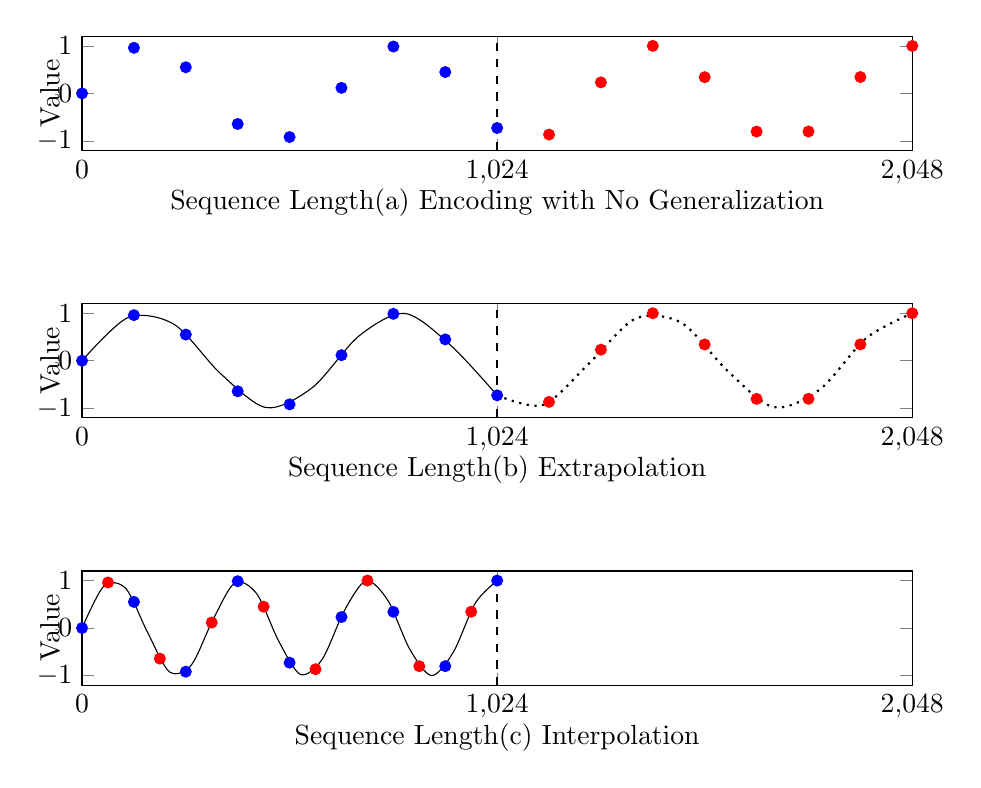
\begin{tikzpicture}
    \begin{axis}[
        at={(0,0)},
        width=\textwidth,
        height=0.25\textwidth,
        title={},
        xlabel={\makecell{Sequence Length\\(a) Encoding with No Generalization}},
        ylabel={Value},
        ylabel style={yshift=-1.5em},xlabel style={yshift=0.5em},
        grid=none,
        xmin=0, xmax=2048,
        xtick={0, 1024, 2048},
        ymin=-1.2, ymax=1.2,
        ytick={-1, 0, 1}
    ]
        % \addplot[
        %     % only marks,
        %     % draw=blue,
        %     % fill=blue,
        %     % mark=*,
        %     domain=0:1024,
        %     samples=5
        % ]{sin(deg(x))};

        \addplot[blue,mark=*,mark size=1.5pt,thick,mark options={fill=blue,draw=blue,line width=1.25pt}, only marks] coordinates {
        (0, sin(0)
        (128, sin(deg(1/100*128)
        (256, sin(deg(1/100*256)
        (384, sin(deg(1/100*384)
        (512, sin(deg(1/100*512)
        (640, sin(deg(1/100*640)
        (768, sin(deg(1/100*768)
        (896, sin(deg(1/100*896)
        (1024, sin(deg(1/100*1024) };

        \addplot[red,mark=*,mark size=1.5pt,thick,mark options={fill=red,draw=red,line width=1.25pt}, only marks] coordinates {
        (1152, sin(deg(1/100*1152)
        (1280, sin(deg(1/100*1280)
        (1408, sin(deg(1/100*1408)
        (1536, sin(deg(1/100*1536)
        (1664, sin(deg(1/100*1664)
        (1792, sin(deg(1/100*1792)
        (1920, sin(deg(1/100*1920)
        (2048, sin(deg(1/100*2048)  };
    \draw[dashed, thick] (axis cs:1024,-1.2) -- (axis cs:1024,1.2);

    \end{axis}

    \begin{axis}[
        at={(0,-0.28\textwidth)},
        width=\textwidth,
        height=0.25\textwidth,
        title={},
        xlabel={\makecell{Sequence Length\\(b) Extrapolation}},
        ylabel={Value},
        ylabel style={yshift=-1.5em},xlabel style={yshift=0.5em},
        grid=none,
        xmin=0, xmax=2048,
        xtick={0, 1024, 2048},
        ymin=-1.2, ymax=1.2,
        ytick={-1, 0, 1}
    ]
        \addplot[
            domain=0:1024,
            samples=10,
            % samples at={0, 1024/11, 1024/11*2, 1024/11*3, 512, 640, 768, 896, 1024},
            smooth,
        ]{sin(deg(1/100*x))};

        \addplot[
            dotted,
            thick,
            domain=1024:2048,
            samples=10,
            % samples at={0, 128, 256, 384, 512, 640, 768, 896, 1024},
            smooth,
        ]{sin(deg(1/100*x))};


    \addplot[blue,mark=*,mark size=1.5pt,thick,mark options={fill=blue,draw=blue,line width=1.25pt}, only marks] coordinates {
        (0, sin(0)
        (128, sin(deg(1/100*128)
        (256, sin(deg(1/100*256)
        (384, sin(deg(1/100*384)
        (512, sin(deg(1/100*512)
        (640, sin(deg(1/100*640)
        (768, sin(deg(1/100*768)
        (896, sin(deg(1/100*896)
        (1024, sin(deg(1/100*1024) };

        \addplot[red,mark=*,mark size=1.5pt,thick,mark options={fill=red,draw=red,line width=1.25pt}, only marks] coordinates {
        (1152, sin(deg(1/100*1152)
        (1280, sin(deg(1/100*1280)
        (1408, sin(deg(1/100*1408)
        (1536, sin(deg(1/100*1536)
        (1664, sin(deg(1/100*1664)
        (1792, sin(deg(1/100*1792)
        (1920, sin(deg(1/100*1920)
        (2048, sin(deg(1/100*2048)  };
    \draw[dashed, thick] (axis cs:1024,-1.2) -- (axis cs:1024,1.2);

    \end{axis}
    \begin{axis}[
        at={(0,-0.56\textwidth)},
        width=\textwidth,
        height=0.25\textwidth,
        title={},
        xlabel={\makecell{Sequence Length\\(c) Interpolation}},
        ylabel={Value},
        ylabel style={yshift=-1.5em},xlabel style={yshift=0.5em},
        grid=none,
        xmin=0, xmax=2048,
        xtick={0, 1024, 2048},
        ymin=-1.2, ymax=1.2,
        ytick={-1, 0, 1}
    ]
          \addplot[
            domain=0:1024,
            samples=20,
            smooth,
        ]{sin(deg(1/50*x))};




    \addplot[blue,mark=*,mark size=1.5pt,thick,mark options={fill=blue,draw=blue,line width=1.25pt}, only marks] coordinates {
        (0, sin(0)
        (128, sin(deg(1/100*2*128)
        (256, sin(deg(1/100*2*256)
        (384, sin(deg(1/100*2*384)
        (512, sin(deg(1/100*2*512)
        (640, sin(deg(1/100*2*640)
        (768, sin(deg(1/100*2*768)
        (896, sin(deg(1/100*2*896)
        (1024, sin(deg(1/100*2*1024)
        };

        \addplot[red,mark=*,mark size=1.5pt,thick,mark options={fill=red,draw=red,line width=1.25pt}, only marks] coordinates {
        (64, sin(deg(1/100*2*64)
        (192, sin(deg(1/100*2*192)
        (320, sin(deg(1/100*2*320)
        (448, sin(deg(1/100*2*448)
        (576, sin(deg(1/100*2*576)
        (704, sin(deg(1/100*2*704)
        (832, sin(deg(1/100*2*832)
        (960, sin(deg(1/100*2*960)
        };
    \draw[dashed, thick] (axis cs:1024,-1.2) -- (axis cs:1024,1.2);

    \end{axis}
    \end{tikzpicture} 
\caption{Illustrations of different positional embedding behaviors across a sequence length continuum. Blue points denote positions explicitly observed during training, while red points denote unseen positions encountered at inference time. In sub-figure (a), the embedding model memorizes the training domain and cannot generalize. In sub-figures (b) and (c), the model successfully generalizes to unseen lengths via extrapolation and interpolation, respectively.}
\label{fig:pe-for-a-range-of-positions}
\end{figure}

There are several approaches to making positional embedding models generalize. They can be grouped into two classes.

\begin{itemize}
\item \vspace{0.5em} \mindex{Extrapolation}. The model learned on observed data points (i.e., positions) can be directly employed to assign meaningful values to data points beyond the original range.  For instance, if a model learns a continuous functional relationship for positions $\{1, \cdots, 10\}$, it can theoretically evaluate that same function at position $15$, maintaining the correct relative distance and geometric properties with respect to earlier tokens. Figure~\ref{fig:pe-for-a-range-of-positions} (b) illustrates this concept, where a function fitted to the training domain smoothly extends to estimate values for out-of-distribution coordinates.
\item \vspace{0.3em} \mindex{Interpolation}. This approach maps a larger range of data points into the original observation range. For example, suppose we have a model designed for numbers in the range $[1,10]$. When given a new range of $[1,20]$, we can scale this down by dividing every number by 2, thereby fitting all numbers into $[1,10]$. This scaling allows us to use the model trained on the range $[1,10]$ to describe data points in the expanded range of $[1,20]$. See Figure~\ref{fig:pe-for-a-range-of-positions} (c) for an illustration of this approach.
\end{itemize}
\vspace{0.5em}

In fact, positional embeddings in many systems have achieved some level of generalization. For example, sinusoidal encoding, the most common positional embedding method, employs sine and cosine functions that can naturally extend to sequences of any length. Although this approach seems direct and simple, it does not perform well when we significantly extend the sequences for processing. In this subsection, we will discuss several alternative methods based on either extrapolation or interpolation.

\subsubsection{Attention with Learnable Biases}

\noindent One problem with Eq. (\ref{eq:long-context-pe-base}) is that the embedding model treats each token independently and therefore ignores the distance between different tokens. A common improvement to this model, known as relative positional embedding, is to consider the pairwise relationship between tokens~\cite{shaw-etal:2018self}. The general idea behind this is to compute the offset between any pair of positions and incorporate it into the self-attention model. One of the simplest forms of self-attention with relative positional embedding is given by
\begin{eqnarray}
\mathrm{Att}_{\mathrm{qkv}}(\mathbf{q}_i,\mathbf{K}_{\le i},\mathbf{V}_{\le i}) & = & \sum_{j=0}^{i} \alpha(i,j) \mathbf{v}_j \\
\alpha(i,j) & = & \mathrm{Softmax} \left(\frac{\mathbf{q}_i \mathbf{k}_{j}^\top + \color{red}{\mathrm{PE}(i,j)}}{\sqrt{d}} + \mathrm{Mask}(i,j) \right). \label{eq:attention-weight-base-T5}
\end{eqnarray}

\noindent The only difference between this model and the original self-attention model is that a bias term $\mathrm{PE}(i,j)$ is added to the query-key product in this new model. Intuitively, $\mathrm{PE}(i,j)$ can be interpreted as a distance penalty for the pair of positions $i$ and $j$. As the distance between $i$ and $j$ increases, $\mathrm{PE}(i,j)$ decreases.

$\mathrm{PE}(i,j)$ can be defined in several different ways. Here, we consider the T5 version of relative positional embedding, called the T5 bias~\cite{raffel-etal:2020exploring}. For each pair of query $\mathbf{q}_i$ and key $\mathbf{k}_j$, the offset between them is defined to be\footnote{For language modeling, a query is only allowed to attend to its left-context, and so we have $i - j \ge 0$. In the more general case of self-attention, where a token can attend to all tokens in the sequence, we may have negative offsets when $i < j$.
}
\begin{eqnarray}
d(i,j) & = & i - j.
\end{eqnarray}

A naive formulation for the bias $\mathrm{PE}(i,j)$ would assign a distinct learnable scalar for every possible discrete offset, i.e., $\mathrm{PE}(i,j) = u_{i-j}$, where $u_{i-j}$ is the parameter tied to the exact distance $i - j$. However, simply assigning a unique value to each offset will restrict the model to offsets observed during training. When $i-j$ is larger than the maximum trained offset, the model cannot generalize.

The T5 bias introduces a generalized version of this approach. Rather than allocating a unique parameter to every possible integer offset, it groups these positional offsets into distinct ``buckets,'' where all offsets mapping to the same bucket share a single learnable parameter. Specifically, given $n_b$ buckets, the allocation strategy is defined as follows:

\begin{itemize}
\item \vspace{0.5em} For the first half of the buckets (indices $0$ to $\lfloor \frac{n_b}{2} \rfloor - 1$), the mapping is one-to-one. Each offset is mapped to a unique bucket: bucket $0 \leftrightarrow$ offset $0$, bucket $1 \leftrightarrow$ offset $1$, and so on. We can express this linear mapping as $b(i - j) = i - j$.
\item \vspace{0.3em} For the remaining half of the buckets (indices $\lfloor \frac{n_b}{2} \rfloor$ to $n_b - 1$), the bucket size increases logarithmically. As a result, larger offsets are grouped into progressively wider bins. For an offset $i - j \ge \lfloor \frac{n_b}{2} \rfloor$, the bucket index is computed as:
    \begin{eqnarray}
    b(i - j) & = & \lfloor \frac{n_b}{2} \rfloor + \left\lfloor \frac{\log(i - j) - \log(\lfloor \frac{n_b}{2} \rfloor)}{\log(\mathrm{dist}_{\mathrm{max}}) - \log(\lfloor \frac{n_b}{2} \rfloor)} \cdot \left(n_b - \lfloor \frac{n_b}{2} \rfloor - 1\right) \right\rfloor,
    \end{eqnarray}
    \noindent where $\mathrm{dist}_{\mathrm{max}}$ is a hyperparameter indicating the maximum expected offset threshold.
\item \vspace{0.3em} When $i - j \ge \mathrm{dist}_{\mathrm{max}}$, the offset is clipped and placed into the final bucket $n_b - 1$. In other words, this bucket serves as a catch-all for any arbitrarily large distances extending beyond the expected sequence length.
\end{itemize}

Together, the bucketing function is defined as
{\small
\begin{eqnarray}
& & b(i - j) \nonumber \\
& = &
\begin{cases}
i - j & \text{if } 0 \le i - j < \lfloor \frac{n_b}{2} \rfloor, \\
\min\left(n_b - 1, \lfloor \frac{n_b}{2} \rfloor + \left\lfloor \frac{\log(i - j) - \log(\lfloor \frac{n_b}{2} \rfloor)}{\log(\mathrm{dist}_{\mathrm{max}}) - \log(\lfloor \frac{n_b}{2} \rfloor)} \cdot \left(n_b - \lfloor \frac{n_b}{2} \rfloor - 1\right) \right\rfloor \right) & \text{if } i - j \ge \lfloor \frac{n_b}{2} \rfloor.
\end{cases} \nonumber \\
\end{eqnarray}
}

Figure~\ref{fig:qk-distances-in-buckets-T5} shows an illustration of these buckets. We see that in the first half of the buckets, each bucket is associated with only one value of $i - j$, while in the second half, the bucket size increases as $i - j$ grows. The last bucket is designed to handle sequences of arbitrary length.

\begin{figure}[!t]
\centering
% !Mode:: "TeX:UTF-8"
% !TEX encoding = UTF-8 Unicode

\begin{center}
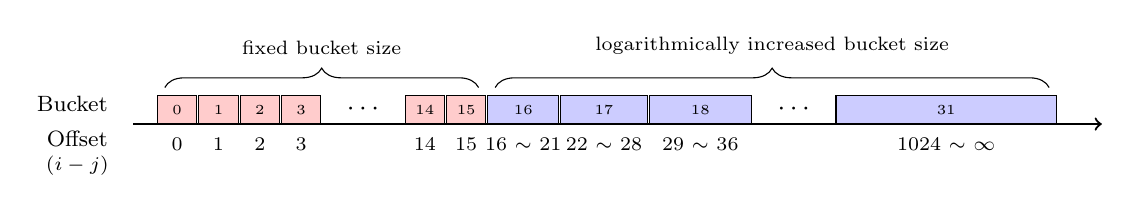
\begin{tikzpicture}
	
\def\ssep{1.0cm}
\def\nsep{0.1cm}

\tikzstyle{snode} = [minimum width=0.5cm,minimum height=0.35cm,inner sep=0pt,draw];

\begin{scope}

\draw [->,thick] (0,0) -- (12.3cm,0);

\node [snode,anchor=south west,fill=red!20] (b0) at (0.3cm,0) {\tiny{0}};
\node [snode,anchor=west,fill=red!20] (b1) at ([xshift=0.3pt]b0.east) {\tiny{1}};
\node [snode,anchor=west,fill=red!20] (b2) at ([xshift=0.3pt]b1.east) {\tiny{2}};
\node [snode,anchor=west,fill=red!20] (b3) at ([xshift=0.3pt]b2.east) {\tiny{3}};
\node [anchor=west] (bdots) at ([xshift=0.2cm]b3.east) {$\cdots$};
\node [snode,anchor=west,fill=red!20] (b14) at ([xshift=0.2cm]bdots.east) {\tiny{14}};
\node [snode,anchor=west,fill=red!20] (b15) at ([xshift=0.3pt]b14.east) {\tiny{15}};
\node [snode,anchor=west,minimum width=0.9cm,fill=blue!20] (b16) at ([xshift=0.3pt]b15.east) {\tiny{16}};
\node [snode,anchor=west,minimum width=1.1cm,fill=blue!20] (b17) at ([xshift=0.3pt]b16.east) {\tiny{17}};
\node [snode,anchor=west,minimum width=1.3cm,fill=blue!20] (b18) at ([xshift=0.3pt]b17.east) {\tiny{18}};
\node [anchor=west] (bdots2) at ([xshift=0.2cm]b18.east) {$\cdots$};
\node [snode,anchor=west,minimum width=2.8cm,fill=blue!20] (b32) at ([xshift=0.2cm]bdots2.east) {\tiny{31}};

\node [anchor=east] (blabel) at ([xshift=-0.5cm,yshift=2pt]b0.west) {\footnotesize{Bucket}};
\node [anchor=north east] (ilabel) at ([yshift=-0.00cm]blabel.south east) {\footnotesize{Offset}};
\node [anchor=north] (ilabel2) at ([yshift=0.13cm]ilabel.south) {\scriptsize{$(i-j)$}};

\node [anchor=north] (d0) at ([yshift=-0.05cm]b0.south) {\scriptsize{0}};
\node [anchor=north] (d1) at ([yshift=-0.05cm]b1.south) {\scriptsize{1}};
\node [anchor=north] (d2) at ([yshift=-0.05cm]b2.south) {\scriptsize{2}};
\node [anchor=north] (d3) at ([yshift=-0.05cm]b3.south) {\scriptsize{3}};
\node [anchor=north] (d15) at ([yshift=-0.05cm]b14.south) {\scriptsize{14}};
\node [anchor=north] (d16) at ([yshift=-0.05cm]b15.south) {\scriptsize{15}};
\node [anchor=north] (d17) at ([yshift=-0.05cm]b16.south) {\scriptsize{16 $\sim$ 21}};
\node [anchor=north] (d18) at ([yshift=-0.05cm]b17.south) {\scriptsize{22 $\sim$ 28}};
\node [anchor=north] (d19) at ([yshift=-0.05cm]b18.south) {\scriptsize{29 $\sim$ 36}};
\node [anchor=north] (d32) at ([yshift=-0.05cm]b32.south) {\scriptsize{1024 $\sim$ $\infty$}};

\draw [decoration={brace,amplitude=7pt},decorate] ([yshift=0.1cm,xshift=0.1cm]b0.north west) --  ([yshift=0.1cm,xshift=-0.1cm]b15.north east) node [pos=0.5,above,yshift=0.3cm] {\scriptsize{fixed bucket size}};
\draw [decoration={brace,amplitude=7pt},decorate] ([yshift=0.1cm,xshift=0.1cm]b16.north west) --  ([yshift=0.1cm,xshift=-0.1cm]b32.north east) node [pos=0.5,above,yshift=0.3cm] {\scriptsize{logarithmically increased bucket size}};

\end{scope}
	
    \end{tikzpicture}
\end{center}

\caption{Illustration of distributing query-key offsets into buckets in the T5 model ($n_b = 32$ and $\mathrm{dist}_{\mathrm{max}}=1024$). Boxes represent buckets. In the first half of the buckets, we use a fixed bucket size. In the second half of the buckets, we increase the bucket size logarithmically. The last bucket contains all the query-key offsets that are not covered by previous buckets.}
\label{fig:qk-distances-in-buckets-T5}
\end{figure}

All relative distances mapping to the same bucket $b(i-j)$ share an identical learnable bias scalar $u_{b(i-j)}$. Substituting $\mathrm{PE}(i,j) = u_{b(i-j)}$ back into Eq. (\ref{eq:attention-weight-base-T5}), the final attention weight computation becomes\footnote{Note that, in~\citet{raffel-etal:2020exploring}'s T5 model, the rescaling operation for the query-key product is removed. The attention weight $\alpha(i,j)$ is then given by
\begin{eqnarray}
\alpha(i,j) & = & \mathrm{Softmax}(\mathbf{q}_i \mathbf{k}_{j}^\top + u_{b(i-j)} + \mathrm{Mask}(i,j)).
\end{eqnarray}
}
\begin{eqnarray}
\alpha(i,j) & = & \mathrm{Softmax}\left( \frac{\mathbf{q}_i \mathbf{k}_{j}^\top + \color{red}{u_{b(i-j)}}}{\sqrt{d}} + \mathrm{Mask}(i,j) \right),
\end{eqnarray}

The parameters $\{u_{0},\cdots,u_{n_b-1}\}$ are learned jointly with other parameters of the model. It should be emphasized that this model can generalize to long sequences. This is because $\mathrm{PE}(i,j)$s with similar query-key offsets share the same parameter, and this sharing strategy is particularly important for achieving good generalization, given that large query-key offsets are rare in training. In practice, we often set $n_b$ to a moderate number, and thus it can help control the overfitting of positional embedding models.

\subsubsection{Attention with Fixed Biases}

\noindent Relative positional embedding models are based on a set of learned biases added to the query-key product in self-attention. An alternative approach is to assign fixed values to these biases via predefined heuristics, rather than learning them from data. One benefit of this heuristic-based approach is that it does not rely on training and thus can be directly applied to any sequence once the biases are set.

One example of such an approach is~\citet{press-etal:2022train}'s approach, called \mindex{attention with linear biases} or \mindex{ALiBi} for short. In the ALiBi approach, the bias term is defined as the negative scaled query-key offset
\begin{eqnarray}
\mathrm{PE}(i,j) & = & -\beta \cdot (i - j) \nonumber \\
                 & = & \beta \cdot (j - i) \label{eq:abili-bias},
\end{eqnarray}

\noindent where $\beta$ is the scaling factor. Adding this term to the query-key product, we obtain a new form of attention weights
\begin{eqnarray}
\alpha(i,j) & = & \mathrm{Softmax} \left(\frac{\mathbf{q}_i \mathbf{k}_{j}^\top + \color{red}{\beta \cdot (j - i)}}{\sqrt{d}} + \mathrm{Mask}(i,j) \right).
\end{eqnarray}

This model can be interpreted as imposing a linear penalty on the attention score $\mathbf{q}_i \mathbf{k}_{j}^\top$ for every step the key $j$ moves away from the query $i$. See Figure~\ref{fig:T5-and-ALiBi-biases} for a comparison of the T5 bias and the ALiBi bias.

\begin{figure}[!t]
\centering
% !Mode:: "TeX:UTF-8"
% !TEX encoding = UTF-8 Unicode

\begin{center}
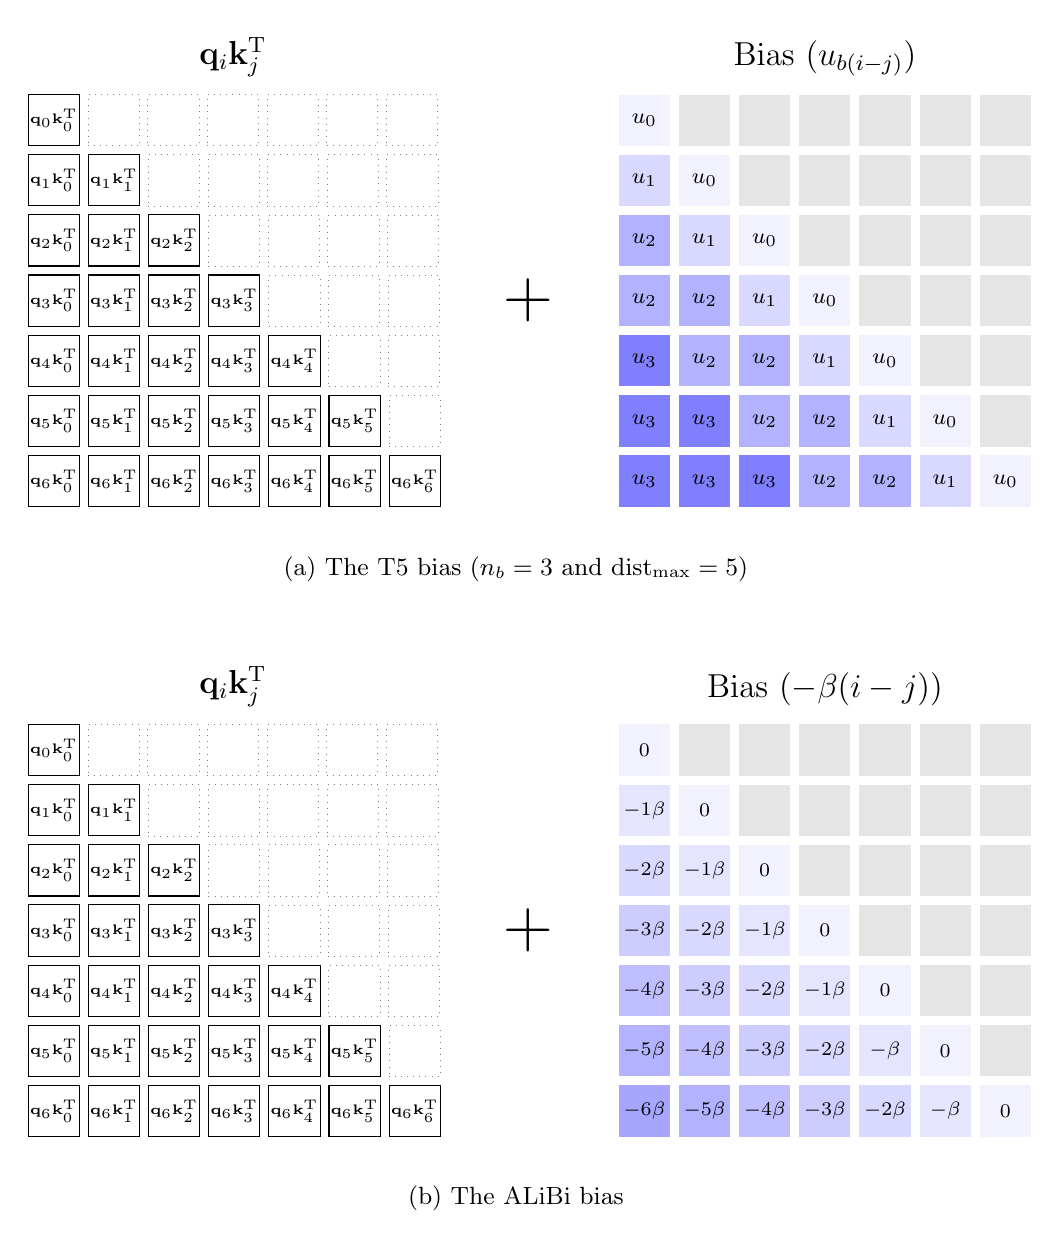
\begin{tikzpicture}
	
\def\ssep{1.0cm}
\def\nsep{0.1cm}

\tikzstyle{snode} = [minimum width=0.65cm,minimum height=0.65cm,inner sep=0pt,draw,thin];
\tikzstyle{bnode} = [minimum width=0.65cm,minimum height=0.65cm,inner sep=0pt,fill=gray!20];

%%%%%%%%%%%%%%%%%%%%%%%%%%%%%%%%%%%
%% sub-figure 1: the T5 bias

\begin{scope}

\node [snode,anchor=west] (c00) at (0,0) {\tiny{$\mathbf{q}_{0} \mathbf{k}_{0}^{\mathrm{T}}$}};
\node [snode,anchor=west,very thin,draw=gray!100,dotted] (c01) at ([xshift=0.1cm]c00.east) {};
\node [snode,anchor=west,very thin,draw=gray!100,dotted] (c02) at ([xshift=0.1cm]c01.east) {};
\node [snode,anchor=west,very thin,draw=gray!100,dotted] (c03) at ([xshift=0.1cm]c02.east) {};
\node [snode,anchor=west,very thin,draw=gray!100,dotted] (c04) at ([xshift=0.1cm]c03.east) {};
\node [snode,anchor=west,very thin,draw=gray!100,dotted] (c05) at ([xshift=0.1cm]c04.east) {};
\node [snode,anchor=west,very thin,draw=gray!100,dotted] (c06) at ([xshift=0.1cm]c05.east) {};

\node [snode,anchor=north] (c10) at ([yshift=-0.1cm]c00.south) {\tiny{$\mathbf{q}_{1} \mathbf{k}_{0}^{\mathrm{T}}$}};
\node [snode,anchor=west] (c11) at ([xshift=0.1cm]c10.east) {\tiny{$\mathbf{q}_{1} \mathbf{k}_{1}^{\mathrm{T}}$}};
\node [snode,anchor=west,very thin,draw=gray!100,dotted] (c12) at ([xshift=0.1cm]c11.east) {};
\node [snode,anchor=west,very thin,draw=gray!100,dotted] (c13) at ([xshift=0.1cm]c12.east) {};
\node [snode,anchor=west,very thin,draw=gray!100,dotted] (c14) at ([xshift=0.1cm]c13.east) {};
\node [snode,anchor=west,very thin,draw=gray!100,dotted] (c15) at ([xshift=0.1cm]c14.east) {};
\node [snode,anchor=west,very thin,draw=gray!100,dotted] (c16) at ([xshift=0.1cm]c15.east) {};

\node [snode,anchor=north] (c20) at ([yshift=-0.1cm]c10.south) {\tiny{$\mathbf{q}_{2} \mathbf{k}_{0}^{\mathrm{T}}$}};
\node [snode,anchor=west] (c21) at ([xshift=0.1cm]c20.east) {\tiny{$\mathbf{q}_{2} \mathbf{k}_{1}^{\mathrm{T}}$}};
\node [snode,anchor=west] (c22) at ([xshift=0.1cm]c21.east) {\tiny{$\mathbf{q}_{2} \mathbf{k}_{2}^{\mathrm{T}}$}};
\node [snode,anchor=west,very thin,draw=gray!100,dotted] (c23) at ([xshift=0.1cm]c22.east) {};
\node [snode,anchor=west,very thin,draw=gray!100,dotted] (c24) at ([xshift=0.1cm]c23.east) {};
\node [snode,anchor=west,very thin,draw=gray!100,dotted] (c25) at ([xshift=0.1cm]c24.east) {};
\node [snode,anchor=west,very thin,draw=gray!100,dotted] (c26) at ([xshift=0.1cm]c25.east) {};

\node [snode,anchor=north] (c30) at ([yshift=-0.1cm]c20.south) {\tiny{$\mathbf{q}_{3} \mathbf{k}_{0}^{\mathrm{T}}$}};
\node [snode,anchor=west] (c31) at ([xshift=0.1cm]c30.east) {\tiny{$\mathbf{q}_{3} \mathbf{k}_{1}^{\mathrm{T}}$}};
\node [snode,anchor=west] (c32) at ([xshift=0.1cm]c31.east) {\tiny{$\mathbf{q}_{3} \mathbf{k}_{2}^{\mathrm{T}}$}};
\node [snode,anchor=west] (c33) at ([xshift=0.1cm]c32.east) {\tiny{$\mathbf{q}_{3} \mathbf{k}_{3}^{\mathrm{T}}$}};
\node [snode,anchor=west,very thin,draw=gray!100,dotted] (c34) at ([xshift=0.1cm]c33.east) {};
\node [snode,anchor=west,very thin,draw=gray!100,dotted] (c35) at ([xshift=0.1cm]c34.east) {};
\node [snode,anchor=west,very thin,draw=gray!100,dotted] (c36) at ([xshift=0.1cm]c35.east) {};

\node [snode,anchor=north] (c40) at ([yshift=-0.1cm]c30.south) {\tiny{$\mathbf{q}_{4} \mathbf{k}_{0}^{\mathrm{T}}$}};
\node [snode,anchor=west] (c41) at ([xshift=0.1cm]c40.east) {\tiny{$\mathbf{q}_{4} \mathbf{k}_{1}^{\mathrm{T}}$}};
\node [snode,anchor=west] (c42) at ([xshift=0.1cm]c41.east) {\tiny{$\mathbf{q}_{4} \mathbf{k}_{2}^{\mathrm{T}}$}};
\node [snode,anchor=west] (c43) at ([xshift=0.1cm]c42.east) {\tiny{$\mathbf{q}_{4} \mathbf{k}_{3}^{\mathrm{T}}$}};
\node [snode,anchor=west] (c44) at ([xshift=0.1cm]c43.east) {\tiny{$\mathbf{q}_{4} \mathbf{k}_{4}^{\mathrm{T}}$}};
\node [snode,anchor=west,very thin,draw=gray!100,dotted] (c45) at ([xshift=0.1cm]c44.east) {};
\node [snode,anchor=west,very thin,draw=gray!100,dotted] (c46) at ([xshift=0.1cm]c45.east) {};

\node [snode,anchor=north] (c50) at ([yshift=-0.1cm]c40.south) {\tiny{$\mathbf{q}_{5} \mathbf{k}_{0}^{\mathrm{T}}$}};
\node [snode,anchor=west] (c51) at ([xshift=0.1cm]c50.east) {\tiny{$\mathbf{q}_{5} \mathbf{k}_{1}^{\mathrm{T}}$}};
\node [snode,anchor=west] (c52) at ([xshift=0.1cm]c51.east) {\tiny{$\mathbf{q}_{5} \mathbf{k}_{2}^{\mathrm{T}}$}};
\node [snode,anchor=west] (c53) at ([xshift=0.1cm]c52.east) {\tiny{$\mathbf{q}_{5} \mathbf{k}_{3}^{\mathrm{T}}$}};
\node [snode,anchor=west] (c54) at ([xshift=0.1cm]c53.east) {\tiny{$\mathbf{q}_{5} \mathbf{k}_{4}^{\mathrm{T}}$}};
\node [snode,anchor=west] (c55) at ([xshift=0.1cm]c54.east) {\tiny{$\mathbf{q}_{5} \mathbf{k}_{5}^{\mathrm{T}}$}};
\node [snode,anchor=west,very thin,draw=gray!100,dotted] (c56) at ([xshift=0.1cm]c55.east) {};

\node [snode,anchor=north] (c60) at ([yshift=-0.1cm]c50.south) {\tiny{$\mathbf{q}_{6} \mathbf{k}_{0}^{\mathrm{T}}$}};
\node [snode,anchor=west] (c61) at ([xshift=0.1cm]c60.east) {\tiny{$\mathbf{q}_{6} \mathbf{k}_{1}^{\mathrm{T}}$}};
\node [snode,anchor=west] (c62) at ([xshift=0.1cm]c61.east) {\tiny{$\mathbf{q}_{6} \mathbf{k}_{2}^{\mathrm{T}}$}};
\node [snode,anchor=west] (c63) at ([xshift=0.1cm]c62.east) {\tiny{$\mathbf{q}_{6} \mathbf{k}_{3}^{\mathrm{T}}$}};
\node [snode,anchor=west] (c64) at ([xshift=0.1cm]c63.east) {\tiny{$\mathbf{q}_{6} \mathbf{k}_{4}^{\mathrm{T}}$}};
\node [snode,anchor=west] (c65) at ([xshift=0.1cm]c64.east) {\tiny{$\mathbf{q}_{6} \mathbf{k}_{5}^{\mathrm{T}}$}};
\node [snode,anchor=west] (c66) at ([xshift=0.1cm]c65.east) {\tiny{$\mathbf{q}_{6} \mathbf{k}_{6}^{\mathrm{T}}$}};

\node [anchor=south] (label) at ([yshift=0.1cm]c03.north) {\large{$\mathbf{q}_i \mathbf{k}_j^{\mathrm{T}}$}};

\end{scope}

\begin{scope}[xshift=7.5cm]

\node [bnode,anchor=west,fill=blue!5] (c00) at (0,0) {\footnotesize{$u_{0}$}};
\node [bnode,anchor=west] (c01) at ([xshift=0.1cm]c00.east) {};
\node [bnode,anchor=west] (c02) at ([xshift=0.1cm]c01.east) {};
\node [bnode,anchor=west] (c03) at ([xshift=0.1cm]c02.east) {};
\node [bnode,anchor=west] (c04) at ([xshift=0.1cm]c03.east) {};
\node [bnode,anchor=west] (c05) at ([xshift=0.1cm]c04.east) {};
\node [bnode,anchor=west] (c06) at ([xshift=0.1cm]c05.east) {};

\node [bnode,anchor=north,fill=blue!15] (c10) at ([yshift=-0.1cm]c00.south) {\footnotesize{$u_{1}$}};
\node [bnode,anchor=west,fill=blue!5] (c11) at ([xshift=0.1cm]c10.east) {\footnotesize{$u_{0}$}};
\node [bnode,anchor=west] (c12) at ([xshift=0.1cm]c11.east) {};
\node [bnode,anchor=west] (c13) at ([xshift=0.1cm]c12.east) {};
\node [bnode,anchor=west] (c14) at ([xshift=0.1cm]c13.east) {};
\node [bnode,anchor=west] (c15) at ([xshift=0.1cm]c14.east) {};
\node [bnode,anchor=west] (c16) at ([xshift=0.1cm]c15.east) {};

\node [bnode,anchor=north,fill=blue!30] (c20) at ([yshift=-0.1cm]c10.south) {\footnotesize{$u_{2}$}};
\node [bnode,anchor=west,fill=blue!15] (c21) at ([xshift=0.1cm]c20.east) {\footnotesize{$u_{1}$}};
\node [bnode,anchor=west,fill=blue!5] (c22) at ([xshift=0.1cm]c21.east) {\footnotesize{$u_{0}$}};
\node [bnode,anchor=west] (c23) at ([xshift=0.1cm]c22.east) {};
\node [bnode,anchor=west] (c24) at ([xshift=0.1cm]c23.east) {};
\node [bnode,anchor=west] (c25) at ([xshift=0.1cm]c24.east) {};
\node [bnode,anchor=west] (c26) at ([xshift=0.1cm]c25.east) {};

\node [bnode,anchor=north,fill=blue!30] (c30) at ([yshift=-0.1cm]c20.south) {\footnotesize{$u_{2}$}};
\node [bnode,anchor=west,fill=blue!30] (c31) at ([xshift=0.1cm]c30.east) {\footnotesize{$u_{2}$}};
\node [bnode,anchor=west,fill=blue!15] (c32) at ([xshift=0.1cm]c31.east) {\footnotesize{$u_{1}$}};
\node [bnode,anchor=west,fill=blue!5] (c33) at ([xshift=0.1cm]c32.east) {\footnotesize{$u_{0}$}};
\node [bnode,anchor=west] (c34) at ([xshift=0.1cm]c33.east) {};
\node [bnode,anchor=west] (c35) at ([xshift=0.1cm]c34.east) {};
\node [bnode,anchor=west] (c36) at ([xshift=0.1cm]c35.east) {};

\node [bnode,anchor=north,fill=blue!50] (c40) at ([yshift=-0.1cm]c30.south) {\footnotesize{$u_{3}$}};
\node [bnode,anchor=west,fill=blue!30] (c41) at ([xshift=0.1cm]c40.east) {\footnotesize{$u_{2}$}};
\node [bnode,anchor=west,fill=blue!30] (c42) at ([xshift=0.1cm]c41.east) {\footnotesize{$u_{2}$}};
\node [bnode,anchor=west,fill=blue!15] (c43) at ([xshift=0.1cm]c42.east) {\footnotesize{$u_{1}$}};
\node [bnode,anchor=west,fill=blue!5] (c44) at ([xshift=0.1cm]c43.east) {\footnotesize{$u_{0}$}};
\node [bnode,anchor=west] (c45) at ([xshift=0.1cm]c44.east) {};
\node [bnode,anchor=west] (c46) at ([xshift=0.1cm]c45.east) {};

\node [bnode,anchor=north,fill=blue!50] (c50) at ([yshift=-0.1cm]c40.south) {\footnotesize{$u_{3}$}};
\node [bnode,anchor=west,fill=blue!50] (c51) at ([xshift=0.1cm]c50.east) {\footnotesize{$u_{3}$}};
\node [bnode,anchor=west,fill=blue!30] (c52) at ([xshift=0.1cm]c51.east) {\footnotesize{$u_{2}$}};
\node [bnode,anchor=west,fill=blue!30] (c53) at ([xshift=0.1cm]c52.east) {\footnotesize{$u_{2}$}};
\node [bnode,anchor=west,fill=blue!15] (c54) at ([xshift=0.1cm]c53.east) {\footnotesize{$u_{1}$}};
\node [bnode,anchor=west,fill=blue!5] (c55) at ([xshift=0.1cm]c54.east) {\footnotesize{$u_{0}$}};
\node [bnode,anchor=west] (c56) at ([xshift=0.1cm]c55.east) {};

\node [bnode,anchor=north,fill=blue!50] (c60) at ([yshift=-0.1cm]c50.south) {\footnotesize{$u_{3}$}};
\node [bnode,anchor=west,fill=blue!50] (c61) at ([xshift=0.1cm]c60.east) {\footnotesize{$u_{3}$}};
\node [bnode,anchor=west,fill=blue!50] (c62) at ([xshift=0.1cm]c61.east) {\footnotesize{$u_{3}$}};
\node [bnode,anchor=west,fill=blue!30] (c63) at ([xshift=0.1cm]c62.east) {\footnotesize{$u_{2}$}};
\node [bnode,anchor=west,fill=blue!30] (c64) at ([xshift=0.1cm]c63.east) {\footnotesize{$u_{2}$}};
\node [bnode,anchor=west,fill=blue!15] (c65) at ([xshift=0.1cm]c64.east) {\footnotesize{$u_{1}$}};
\node [bnode,anchor=west,fill=blue!5] (c66) at ([xshift=0.1cm]c65.east) {\footnotesize{$u_{0}$}};

\node [anchor=south] (label) at ([yshift=0.1cm]c03.north) {\large{Bias ($u_{b(i-j)}$)}};

\node [anchor=east] (addition) at ([xshift=-0.7cm]c30.west) {\Huge{$+$}};

\node [anchor=north] (caption) at ([xshift=-1.3cm,yshift=-0.5cm]c60.south west) {\small{(a) The T5 bias ($n_b = 3$ and $\mathrm{dist}_{\mathrm{max}}=5$)}};

\end{scope}

%%%%%%%%%%%%%%%%%%%%%%%%%%%%%%%%%%%
%% sub-figure 2: the Alibi bias

\begin{scope}[yshift=-8cm]

\node [snode,anchor=west] (c00) at (0,0) {\tiny{$\mathbf{q}_{0} \mathbf{k}_{0}^{\mathrm{T}}$}};
\node [snode,anchor=west,very thin,draw=gray!100,dotted] (c01) at ([xshift=0.1cm]c00.east) {};
\node [snode,anchor=west,very thin,draw=gray!100,dotted] (c02) at ([xshift=0.1cm]c01.east) {};
\node [snode,anchor=west,very thin,draw=gray!100,dotted] (c03) at ([xshift=0.1cm]c02.east) {};
\node [snode,anchor=west,very thin,draw=gray!100,dotted] (c04) at ([xshift=0.1cm]c03.east) {};
\node [snode,anchor=west,very thin,draw=gray!100,dotted] (c05) at ([xshift=0.1cm]c04.east) {};
\node [snode,anchor=west,very thin,draw=gray!100,dotted] (c06) at ([xshift=0.1cm]c05.east) {};

\node [snode,anchor=north] (c10) at ([yshift=-0.1cm]c00.south) {\tiny{$\mathbf{q}_{1} \mathbf{k}_{0}^{\mathrm{T}}$}};
\node [snode,anchor=west] (c11) at ([xshift=0.1cm]c10.east) {\tiny{$\mathbf{q}_{1} \mathbf{k}_{1}^{\mathrm{T}}$}};
\node [snode,anchor=west,very thin,draw=gray!100,dotted] (c12) at ([xshift=0.1cm]c11.east) {};
\node [snode,anchor=west,very thin,draw=gray!100,dotted] (c13) at ([xshift=0.1cm]c12.east) {};
\node [snode,anchor=west,very thin,draw=gray!100,dotted] (c14) at ([xshift=0.1cm]c13.east) {};
\node [snode,anchor=west,very thin,draw=gray!100,dotted] (c15) at ([xshift=0.1cm]c14.east) {};
\node [snode,anchor=west,very thin,draw=gray!100,dotted] (c16) at ([xshift=0.1cm]c15.east) {};

\node [snode,anchor=north] (c20) at ([yshift=-0.1cm]c10.south) {\tiny{$\mathbf{q}_{2} \mathbf{k}_{0}^{\mathrm{T}}$}};
\node [snode,anchor=west] (c21) at ([xshift=0.1cm]c20.east) {\tiny{$\mathbf{q}_{2} \mathbf{k}_{1}^{\mathrm{T}}$}};
\node [snode,anchor=west] (c22) at ([xshift=0.1cm]c21.east) {\tiny{$\mathbf{q}_{2} \mathbf{k}_{2}^{\mathrm{T}}$}};
\node [snode,anchor=west,very thin,draw=gray!100,dotted] (c23) at ([xshift=0.1cm]c22.east) {};
\node [snode,anchor=west,very thin,draw=gray!100,dotted] (c24) at ([xshift=0.1cm]c23.east) {};
\node [snode,anchor=west,very thin,draw=gray!100,dotted] (c25) at ([xshift=0.1cm]c24.east) {};
\node [snode,anchor=west,very thin,draw=gray!100,dotted] (c26) at ([xshift=0.1cm]c25.east) {};

\node [snode,anchor=north] (c30) at ([yshift=-0.1cm]c20.south) {\tiny{$\mathbf{q}_{3} \mathbf{k}_{0}^{\mathrm{T}}$}};
\node [snode,anchor=west] (c31) at ([xshift=0.1cm]c30.east) {\tiny{$\mathbf{q}_{3} \mathbf{k}_{1}^{\mathrm{T}}$}};
\node [snode,anchor=west] (c32) at ([xshift=0.1cm]c31.east) {\tiny{$\mathbf{q}_{3} \mathbf{k}_{2}^{\mathrm{T}}$}};
\node [snode,anchor=west] (c33) at ([xshift=0.1cm]c32.east) {\tiny{$\mathbf{q}_{3} \mathbf{k}_{3}^{\mathrm{T}}$}};
\node [snode,anchor=west,very thin,draw=gray!100,dotted] (c34) at ([xshift=0.1cm]c33.east) {};
\node [snode,anchor=west,very thin,draw=gray!100,dotted] (c35) at ([xshift=0.1cm]c34.east) {};
\node [snode,anchor=west,very thin,draw=gray!100,dotted] (c36) at ([xshift=0.1cm]c35.east) {};

\node [snode,anchor=north] (c40) at ([yshift=-0.1cm]c30.south) {\tiny{$\mathbf{q}_{4} \mathbf{k}_{0}^{\mathrm{T}}$}};
\node [snode,anchor=west] (c41) at ([xshift=0.1cm]c40.east) {\tiny{$\mathbf{q}_{4} \mathbf{k}_{1}^{\mathrm{T}}$}};
\node [snode,anchor=west] (c42) at ([xshift=0.1cm]c41.east) {\tiny{$\mathbf{q}_{4} \mathbf{k}_{2}^{\mathrm{T}}$}};
\node [snode,anchor=west] (c43) at ([xshift=0.1cm]c42.east) {\tiny{$\mathbf{q}_{4} \mathbf{k}_{3}^{\mathrm{T}}$}};
\node [snode,anchor=west] (c44) at ([xshift=0.1cm]c43.east) {\tiny{$\mathbf{q}_{4} \mathbf{k}_{4}^{\mathrm{T}}$}};
\node [snode,anchor=west,very thin,draw=gray!100,dotted] (c45) at ([xshift=0.1cm]c44.east) {};
\node [snode,anchor=west,very thin,draw=gray!100,dotted] (c46) at ([xshift=0.1cm]c45.east) {};

\node [snode,anchor=north] (c50) at ([yshift=-0.1cm]c40.south) {\tiny{$\mathbf{q}_{5} \mathbf{k}_{0}^{\mathrm{T}}$}};
\node [snode,anchor=west] (c51) at ([xshift=0.1cm]c50.east) {\tiny{$\mathbf{q}_{5} \mathbf{k}_{1}^{\mathrm{T}}$}};
\node [snode,anchor=west] (c52) at ([xshift=0.1cm]c51.east) {\tiny{$\mathbf{q}_{5} \mathbf{k}_{2}^{\mathrm{T}}$}};
\node [snode,anchor=west] (c53) at ([xshift=0.1cm]c52.east) {\tiny{$\mathbf{q}_{5} \mathbf{k}_{3}^{\mathrm{T}}$}};
\node [snode,anchor=west] (c54) at ([xshift=0.1cm]c53.east) {\tiny{$\mathbf{q}_{5} \mathbf{k}_{4}^{\mathrm{T}}$}};
\node [snode,anchor=west] (c55) at ([xshift=0.1cm]c54.east) {\tiny{$\mathbf{q}_{5} \mathbf{k}_{5}^{\mathrm{T}}$}};
\node [snode,anchor=west,very thin,draw=gray!100,dotted] (c56) at ([xshift=0.1cm]c55.east) {};

\node [snode,anchor=north] (c60) at ([yshift=-0.1cm]c50.south) {\tiny{$\mathbf{q}_{6} \mathbf{k}_{0}^{\mathrm{T}}$}};
\node [snode,anchor=west] (c61) at ([xshift=0.1cm]c60.east) {\tiny{$\mathbf{q}_{6} \mathbf{k}_{1}^{\mathrm{T}}$}};
\node [snode,anchor=west] (c62) at ([xshift=0.1cm]c61.east) {\tiny{$\mathbf{q}_{6} \mathbf{k}_{2}^{\mathrm{T}}$}};
\node [snode,anchor=west] (c63) at ([xshift=0.1cm]c62.east) {\tiny{$\mathbf{q}_{6} \mathbf{k}_{3}^{\mathrm{T}}$}};
\node [snode,anchor=west] (c64) at ([xshift=0.1cm]c63.east) {\tiny{$\mathbf{q}_{6} \mathbf{k}_{4}^{\mathrm{T}}$}};
\node [snode,anchor=west] (c65) at ([xshift=0.1cm]c64.east) {\tiny{$\mathbf{q}_{6} \mathbf{k}_{5}^{\mathrm{T}}$}};
\node [snode,anchor=west] (c66) at ([xshift=0.1cm]c65.east) {\tiny{$\mathbf{q}_{6} \mathbf{k}_{6}^{\mathrm{T}}$}};

\node [anchor=south] (label) at ([yshift=0.1cm]c03.north) {\large{$\mathbf{q}_i \mathbf{k}_j^{\mathrm{T}}$}};

\end{scope}

\begin{scope}[xshift=7.5cm,yshift=-8cm]

\node [bnode,anchor=west,fill=blue!5] (c00) at (0,0) {\scriptsize{$0$}};
\node [bnode,anchor=west] (c01) at ([xshift=0.1cm]c00.east) {};
\node [bnode,anchor=west] (c02) at ([xshift=0.1cm]c01.east) {};
\node [bnode,anchor=west] (c03) at ([xshift=0.1cm]c02.east) {};
\node [bnode,anchor=west] (c04) at ([xshift=0.1cm]c03.east) {};
\node [bnode,anchor=west] (c05) at ([xshift=0.1cm]c04.east) {};
\node [bnode,anchor=west] (c06) at ([xshift=0.1cm]c05.east) {};

\node [bnode,anchor=north,fill=blue!10] (c10) at ([yshift=-0.1cm]c00.south) {\scriptsize{$-1\beta$}};
\node [bnode,anchor=west,fill=blue!5] (c11) at ([xshift=0.1cm]c10.east) {\scriptsize{$0$}};
\node [bnode,anchor=west] (c12) at ([xshift=0.1cm]c11.east) {};
\node [bnode,anchor=west] (c13) at ([xshift=0.1cm]c12.east) {};
\node [bnode,anchor=west] (c14) at ([xshift=0.1cm]c13.east) {};
\node [bnode,anchor=west] (c15) at ([xshift=0.1cm]c14.east) {};
\node [bnode,anchor=west] (c16) at ([xshift=0.1cm]c15.east) {};

\node [bnode,anchor=north,fill=blue!15] (c20) at ([yshift=-0.1cm]c10.south) {\scriptsize{$-2\beta$}};
\node [bnode,anchor=west,fill=blue!10] (c21) at ([xshift=0.1cm]c20.east) {\scriptsize{$-1\beta$}};
\node [bnode,anchor=west,fill=blue!5] (c22) at ([xshift=0.1cm]c21.east) {\scriptsize{$0$}};
\node [bnode,anchor=west] (c23) at ([xshift=0.1cm]c22.east) {};
\node [bnode,anchor=west] (c24) at ([xshift=0.1cm]c23.east) {};
\node [bnode,anchor=west] (c25) at ([xshift=0.1cm]c24.east) {};
\node [bnode,anchor=west] (c26) at ([xshift=0.1cm]c25.east) {};

\node [bnode,anchor=north,fill=blue!20] (c30) at ([yshift=-0.1cm]c20.south) {\scriptsize{$-3\beta$}};
\node [bnode,anchor=west,fill=blue!15] (c31) at ([xshift=0.1cm]c30.east) {\scriptsize{$-2\beta$}};
\node [bnode,anchor=west,fill=blue!10] (c32) at ([xshift=0.1cm]c31.east) {\scriptsize{$-1\beta$}};
\node [bnode,anchor=west,fill=blue!5] (c33) at ([xshift=0.1cm]c32.east) {\scriptsize{$0$}};
\node [bnode,anchor=west] (c34) at ([xshift=0.1cm]c33.east) {};
\node [bnode,anchor=west] (c35) at ([xshift=0.1cm]c34.east) {};
\node [bnode,anchor=west] (c36) at ([xshift=0.1cm]c35.east) {};

\node [bnode,anchor=north,fill=blue!25] (c40) at ([yshift=-0.1cm]c30.south) {\scriptsize{$-4\beta$}};
\node [bnode,anchor=west,fill=blue!20] (c41) at ([xshift=0.1cm]c40.east) {\scriptsize{$-3\beta$}};
\node [bnode,anchor=west,fill=blue!15] (c42) at ([xshift=0.1cm]c41.east) {\scriptsize{$-2\beta$}};
\node [bnode,anchor=west,fill=blue!10] (c43) at ([xshift=0.1cm]c42.east) {\scriptsize{$-1\beta$}};
\node [bnode,anchor=west,fill=blue!5] (c44) at ([xshift=0.1cm]c43.east) {\scriptsize{$0$}};
\node [bnode,anchor=west] (c45) at ([xshift=0.1cm]c44.east) {};
\node [bnode,anchor=west] (c46) at ([xshift=0.1cm]c45.east) {};

\node [bnode,anchor=north,fill=blue!30] (c50) at ([yshift=-0.1cm]c40.south) {\scriptsize{$-5\beta$}};
\node [bnode,anchor=west,fill=blue!25] (c51) at ([xshift=0.1cm]c50.east) {\scriptsize{$-4\beta$}};
\node [bnode,anchor=west,fill=blue!20] (c52) at ([xshift=0.1cm]c51.east) {\scriptsize{$-3\beta$}};
\node [bnode,anchor=west,fill=blue!15] (c53) at ([xshift=0.1cm]c52.east) {\scriptsize{$-2\beta$}};
\node [bnode,anchor=west,fill=blue!10] (c54) at ([xshift=0.1cm]c53.east) {\scriptsize{$-\beta$}};
\node [bnode,anchor=west,fill=blue!5] (c55) at ([xshift=0.1cm]c54.east) {\scriptsize{$0$}};
\node [bnode,anchor=west] (c56) at ([xshift=0.1cm]c55.east) {};

\node [bnode,anchor=north,fill=blue!35] (c60) at ([yshift=-0.1cm]c50.south) {\scriptsize{$-6\beta$}};
\node [bnode,anchor=west,fill=blue!30] (c61) at ([xshift=0.1cm]c60.east) {\scriptsize{$-5\beta$}};
\node [bnode,anchor=west,fill=blue!25] (c62) at ([xshift=0.1cm]c61.east) {\scriptsize{$-4\beta$}};
\node [bnode,anchor=west,fill=blue!20] (c63) at ([xshift=0.1cm]c62.east) {\scriptsize{$-3\beta$}};
\node [bnode,anchor=west,fill=blue!15] (c64) at ([xshift=0.1cm]c63.east) {\scriptsize{$-2\beta$}};
\node [bnode,anchor=west,fill=blue!10] (c65) at ([xshift=0.1cm]c64.east) {\scriptsize{$-\beta$}};
\node [bnode,anchor=west,fill=blue!5] (c66) at ([xshift=0.1cm]c65.east) {\scriptsize{$0$}};

\node [anchor=south] (label) at ([yshift=0.1cm]c03.north) {\large{Bias ($-\beta (i - j)$)}};

\node [anchor=east] (addition) at ([xshift=-0.7cm]c30.west) {\Huge{$+$}};

\node [anchor=north] (caption) at ([xshift=-1.3cm,yshift=-0.5cm]c60.south west) {\small{(b) The ALiBi bias}};

\end{scope}
	
\end{tikzpicture}
\end{center}

\caption{Query-key products with biases (above = the T5 bias and below = the ALiBi bias). The color scale of the biases ranges from light blue denoting small absolute values to deep blue denoting large absolute values.}
\label{fig:T5-and-ALiBi-biases}
\end{figure}

In principle, the scalar hyperparameter $\beta$ could be tuned via grid search on a validation dataset. However, \citet{press-etal:2022train} demonstrated that setting $\beta$ systematically across attention heads yields strong performance across a variety of tasks without any tuning. Specifically, for a multi-head self-attention layer comprising $n_{\mathrm{head}}$ heads, the $\beta$ values decrease geometrically. The scalar for the $k$-th head is defined as
\begin{eqnarray}
\beta_k & = & 2^{-\frac{8k}{n_{\mathrm{head}}}}. \label{eq:alibi-beta}
\end{eqnarray}

The ALiBi approach provides a simple form of relative positional embeddings. There are other similar methods for designing query-key biases using the offset $i - j$. Table~\ref{tab:query-key-biases-comparison} shows a comparison of such biases. As an aside, it is worth noting that the form of the right-hand side of Eq. (\ref{eq:abili-bias}) is similar to distance-based features used in conventional feature-based systems. For example, in statistical machine translation systems, such features are widely used to model word reordering problems, resulting in models that can generalize well across different translation tasks~\cite{Koehn:2010}.

\begin{table}[t]
\centering
\begingroup
\renewcommand{\arraystretch}{1.2}
\begin{tabular}{l | l}
Entry & Query-Key Bias ($\mathrm{PE}(i,j)$) \\ \hline
T5~\cite{raffel-etal:2020exploring} & $u_{b(i-j)}$ \\ \hline
ALiBi~\cite{press-etal:2022train} & $-\beta \cdot (\colorbox{gray!30}{$i - j$})$ \\ \hline
Kerple~\cite{chi-etal:2022kerple} & $-\beta_1 (\colorbox{gray!30}{$i - j$})^{\beta_2}$ \ \ \ (power) \\
                                  & $-\beta_1 \log(1 + \beta_2(\colorbox{gray!30}{$i - j$}))$ \ \ \ (logarithmic)\\ \hline
Sandwich~\cite{chi-etal:2023dissecting} & $\sum_{k=1}^{\bar{d}/2} \cos\big((\colorbox{gray!30}{$i - j$})/10000^{2k/\bar{d}} \big)$ \\ \hline
FIRE~\cite{li-etal:2024functional} & $f\big( \psi(\colorbox{gray!30}{$i - j$})/\psi(\max(m_{\mathrm{len}},i)) \big)$
\end{tabular}
\endgroup
\caption{Query-key biases as relative positional embeddings. $\beta$, $\beta_1$, $\beta_2$, $\bar{d}$, and $m_{\mathrm{len}}$ are hyper-parameters. In the T5 model, $b(i-j)$ denotes the bucket assigned to $i - j$. In the FIRE model, $\psi(\cdot)$ represents a monotonically increasing bounding function, such as $\psi(x) = \log(cx+1)$, and $f(\cdot)$ is an FFN.}
\label{tab:query-key-biases-comparison}
\end{table}

\subsubsection{Rotary Positional Embedding}

\noindent Similar to sinusoidal embeddings, rotary positional embeddings use predefined frequency scales~\cite{su-etal:2024roformer}. Recall that in the sinusoidal embedding model, absolute positions are represented as fixed vectors composed of sine and cosine functions with varying frequencies, which are then additively combined with token embeddings. Rotary positional embeddings, instead, model positional context by applying geometrically meaningful rotations to token embeddings in the complex domain. This yields a formulation based on multiplicative interactions:
\begin{eqnarray}
\mathbf{e}_i & = & \mathbf{x}_i R(i) \label{eq:additive-embedding-e-base},
\end{eqnarray}

\noindent where $R(i) \in \mathbb{R}^{d \times d}$ is the rotation matrix representing the rotations performed on the token embedding $\mathbf{x}_i \in \mathbb{R}^{d}$.

For simplicity, we will first consider embeddings with only two dimensions and return to a discussion of the more general formulation later. Suppose we have a 2-dimensional token embedding represented as a row vector $\mathbf{x} = \begin{bmatrix} x_1 & x_2 \end{bmatrix}$. We can represent it as a vector in a plane, originating at the origin $(0,0)$ and terminating at $(x_1, x_2)$. A counterclockwise rotation of this vector refers to an operation of moving the vector around the origin while maintaining its magnitude, as shown in Figure~\ref{fig:vector-rotation} (a). The degree of rotation is usually defined by a specific angle, denoted by $\theta$. The rotation can be expressed mathematically in the form
\begin{eqnarray}
\mathrm{Ro}(\mathbf{x},\theta) & = & \mathbf{x} R_{\theta} \nonumber \\
                               & = & \begin{bmatrix} x_1 & x_2 \end{bmatrix}
                                     \begin{bmatrix} \cos \theta & \sin \theta \\ -\sin \theta & \cos \theta \end{bmatrix} \nonumber \\
                               & = & \begin{bmatrix} \cos \theta \cdot x_1 - \sin \theta \cdot x_2 & \sin \theta \cdot x_1 + \cos \theta \cdot x_2 \end{bmatrix}.
\end{eqnarray}

\begin{figure}[!t]
\centering
% !Mode:: "TeX:UTF-8"
% !TEX encoding = UTF-8 Unicode

\begin{center}
\begin{tikzpicture}
	
\def\ssep{1.0cm}
\def\nsep{0.1cm}
\def\psize{2.5cm}
\def\rsize{0.7*\psize}

\tikzstyle{snode} = [minimum width=0.65cm,minimum height=0.65cm,inner sep=0pt,draw,thin];
\tikzstyle{bnode} = [minimum width=0.65cm,minimum height=0.65cm,inner sep=0pt,fill=gray!20];

%%%%%%%%%%%%%%%%%%%%%%%%%%%%%%%%%%%
%% sub-figure 1: single-step rotation

\begin{scope}

\draw [-latex,thick] (-\psize,0) -- (\psize,0) node [pos=0.95,below] {\footnotesize{$x_1$}};
\draw [-latex,thick] (0,-\psize) -- (0,\psize) node [pos=0.95,left] {\footnotesize{$x_2$}};

\node [circle,minimum size=2*\rsize,draw] (helpline) at (0,0) {};

\coordinate (O) at (0,0);
\coordinate (A) at (0.5*\rsize,0.8660254*\rsize); % angle = 60
\coordinate (B) at (-0.8660254*\rsize,0.5*\rsize); % angle = 150

\draw [-latex,blue,very thick] (O) -- (A);
\draw [-latex,blue,very thick] (O) -- (B);

\pic[draw,->,thick,red,"$\theta$", angle eccentricity=1.5] {angle = A--O--B};

\node [anchor=south] (labela) at ([yshift=0.0cm,xshift=0.5cm]A) {\footnotesize{vector $\mathbf{x}$}};
\node [anchor=south] (labelb) at ([yshift=0.0cm,xshift=-0.3cm]B) {\footnotesize{$\mathbf{x} R_{\theta}$}};
\node [anchor=south east] (labelb2) at ([yshift=-0.1cm]labelb.north east) {\footnotesize{rotated vector}};

\node [anchor=north] (caption) at (0,-\psize-0.2cm) {\small{(a) Single-step Rotation}};

\end{scope}

%%%%%%%%%%%%%%%%%%%%%%%%%%%%%%%%%%%
%% sub-figure 2: multi-step rotation

\begin{scope}[xshift=7cm]

\draw [-latex,thick] (-\psize,0) -- (\psize,0) node [pos=0.95,below] {\footnotesize{$x_1$}};
\draw [-latex,thick] (0,-\psize) -- (0,\psize) node [pos=0.95,left] {\footnotesize{$x_2$}};

\node [circle,minimum size=2*\rsize,draw] (helpline) at (0,0) {};

\coordinate (O) at (0,0);
\coordinate (A) at (0.5*\rsize,0.8660254*\rsize); % angle = 60
\coordinate (B) at (-0.70711*\rsize,0.70711*\rsize); % angle = 135
\coordinate (C) at (-0.86603*\rsize,-0.50000*\rsize); % angle = 210
\coordinate (D) at (0.25882*\rsize,-0.96593*\rsize); % angle = 285

\draw [-latex,blue,very thick] (O) -- (A);
\draw [-latex,blue,very thick,dotted] (O) -- (B);
\draw [-latex,blue,very thick,dotted] (O) -- (C);
\draw [-latex,blue,very thick] (O) -- (D);

\pic[draw,->,thick,red,"$\theta$", angle radius=0.3*\rsize, angle eccentricity=1.5] {angle = A--O--B};
\pic[draw,->,thick,red,"$\theta$", angle radius=0.4*\rsize,angle eccentricity=1.5] {angle = B--O--C};
\pic[draw,->,thick,red,"$\theta$", angle radius=0.5*\rsize, angle eccentricity=1.5] {angle = C--O--D};

\node [anchor=south] (labela) at ([yshift=0.0cm,xshift=0.2cm]A) {\footnotesize{$\mathbf{x}$}};
\node [anchor=south] (labelb) at ([yshift=0.0cm,xshift=-0.3cm]B) {\footnotesize{$\mathbf{x} R_{\theta}$}};
\node [anchor=east] (labelc) at ([yshift=-0.2cm,xshift=0.1cm]C) {\footnotesize{$\mathbf{x} R_{2\theta}$}};
\node [anchor=north] (labeld) at ([yshift=-0.1cm,xshift=0.1cm]D) {\footnotesize{$\mathbf{x} R_{3\theta}$}};

\node [anchor=north] (caption) at (0,-\psize-0.2cm) {\small{(b) Multi-step Rotation}};

\end{scope}

%%%%%%%%%%%%%%%%%%%%%%%%%%%%%%%%%%%
%% sub-figure 3: angles between embeddings of different tokens

\begin{scope}[xshift=3.5cm,yshift=-7cm]

\draw [-latex,thick] (-\psize,0) -- (\psize,0) node [pos=0.95,below] {\footnotesize{$x_1$}};
\draw [-latex,thick] (0,-\psize) -- (0,\psize) node [pos=0.95,left] {\footnotesize{$x_2$}};

\node [circle,minimum size=2*\rsize,draw] (helpline) at (0,0) {};
\node [circle,minimum size=0.7*2*\rsize,draw] (helpline2) at (0,0) {};

\coordinate (O) at (0,0);
\coordinate (A) at (0.5*\rsize,0.8660254*\rsize); % angle = 60
\coordinate (B) at (-0.8660254*\rsize,-0.5*\rsize); % angle = 210
\coordinate (A2) at (-0.17365*0.7*\rsize,0.98481*0.7*\rsize); % angle = 100
\coordinate (B2) at (-0.34202*0.7*\rsize,-0.93969*0.7*\rsize); % angle = 210

\pic[draw,->,thick,red,"$7\theta$",angle radius=0.8*\rsize,angle eccentricity=1.15] {angle = A--O--B};
\pic[draw,->,thick,red,"$7\theta$",angle radius=0.5*\rsize,angle eccentricity=1.25] {angle = A2--O--B2};
\pic[fill=gray!40,angle radius=0.3*\rsize] {angle = A--O--A2};
\pic[fill=gray!40,angle radius=0.3*\rsize] {angle = B--O--B2};

\draw [-latex,blue,very thick] (O) -- (A);
\draw [-latex,blue,very thick] (O) -- (B);
\draw [-latex,ugreen,very thick] (O) -- (A2);
\draw [-latex,ugreen,very thick] (O) -- (B2);

\node [anchor=south] (labela) at ([yshift=0.0cm,xshift=0.3cm]A) {\scriptsize{sleeping$_4$}};
\node [anchor=south] (labelb) at ([yshift=-0.4cm,xshift=-0.6cm]B) {\scriptsize{sleeping$_{11}$}};
\node [anchor=south,fill=white,inner sep=1pt] (labela2) at ([yshift=-0.4cm,xshift=-0.4cm]A2) {\scriptsize{cat$_2$}};
\node [anchor=south,fill=white,inner sep=1pt] (labelb2) at ([yshift=-0.4cm,xshift=-0.0cm]B2) {\scriptsize{cat$_9$}};

\node [anchor=south west] (senta) at ([yshift=1cm]A) {\footnotesize{{\color{gray} The$_1$} cat$_2$ {\color{gray} is$_3$} sleeping$_4$ {\color{gray} peacefully$_5$} }};
\node [anchor=north west] (senta2) at ([yshift=0.1cm]senta.south west) {\footnotesize{{\color{gray} in$_6$ the$_7$ warm$_8$ sunlight$_9$ .$_{10}$}}};
\node [anchor=north east] (sentb) at ([yshift=-0.5cm]B) {\footnotesize{{\color{gray} Every$_1$ afternoon$_2$ ,$_3$ you$_4$ 'll$_5$ find$_6$ that$_7$}}};
\node [anchor=north west] (sentb2) at ([yshift=0.1cm]sentb.south west) {\footnotesize{{\color{gray} the$_8$} cat$_9$ {\color{gray} is$_{10}$} sleeping$_{11}$ {\color{gray} on$_{12}$ my$_{13}$ bed$_{14}$ .$_{15}$}}};

\node [anchor=north] (caption) at (0,-\psize-0.2cm) {\small{(c) Angles between embeddings of two tokens at different positions}};

\end{scope}

	
\end{tikzpicture}
\end{center}

\caption{Illustrations of vector rotations in a plane. Sub-figures (a) and (b) show rotations of a vector in a single step and multiple steps, respectively. Sub-figure (c) shows the embeddings of tokens \textit{cat} and \textit{sleeping} in two different sentences. We show these sentences with a subscript affixed to each token to indicate its position. If we represent tokens as vectors, we can add positional information by rotating these vectors. This rotation preserves the ``distances'' between the vectors. For example, given that the distance between \textit{cat} and \textit{sleeping} is the same in both sentences, the angle between their embeddings also remains the same during rotation.}
\label{fig:vector-rotation}
\end{figure}

\noindent where $R_{\theta} = \begin{bmatrix} \cos \theta & \sin \theta \\ -\sin \theta & \cos \theta \end{bmatrix}$ is the rotation matrix. If two or more rotations are performed on the same vector, we can rotate the vector further. This follows from the fact that the composition of successive rotations is itself a rotation. More formally, rotating a vector by an angle $\theta$, repeated $t$ times, can be expressed as
\begin{eqnarray}
\mathrm{Ro}(\mathbf{x},t\theta) & = & \mathbf{x} R_{t \theta} \nonumber \\
                                & = & \begin{bmatrix} \cos t \theta \cdot x_1 - \sin t \theta \cdot x_2 & \sin t \theta \cdot x_1 + \cos t \theta \cdot x_2 \end{bmatrix}.
\end{eqnarray}

If we interpret $t$ as the position of a token represented by $\mathbf{x}$ in a sequence, then we will find that the above equation defines a simple positional embedding model. As shown in Figure~\ref{fig:vector-rotation} (b), we start moving the token from position 0. Each time we move one step forward, the vector is rotated by the angle $\theta$. Upon arriving at the position $t$, the representation of the token with positional context is given by $\mathrm{Ro}(\mathbf{x},t\theta)$. As the rotations do not change the magnitude of the embedding, the original ``meaning'' of the token is retained. The positional information is injected into the embedding when it gets rotated.

A common way to understand vector rotation is via complex numbers. It is easy to transform each vector $\mathbf{x} = \begin{bmatrix} x_1 & x_2 \end{bmatrix}$ in the 2D Euclidean space $\mathbb{R}^2$ to a complex number $\mathbf{x}' = x_1 + \mathtt{i} x_2$ in the complex space $\mathbb{C}$ via a bijective linear map. Then, the rotation of $\mathbf{x}$ with the angle $t\theta$ corresponds to the multiplication by $e^{\mathtt{i} t\theta}$. Given that $e^{\mathtt{i} t\theta} = \cos t \theta + \mathtt{i} \sin t \theta$, the rotation operation can be re-expressed in the form
\begin{eqnarray}
\mathbf{x} R_{t \theta} & \mapsto & \mathbf{x}' e^{\mathtt{i} t\theta} \nonumber \\
                        & =       & (x_1 + \mathtt{i} x_2) (\cos t \theta + \mathtt{i} \sin t \theta) \nonumber \\
                        & =       & \cos t \theta \cdot x_1 - \sin t \theta \cdot x_2 + \mathtt{i} (\sin t \theta \cdot x_1 + \cos t \theta \cdot x_2).
\end{eqnarray}

\noindent Here we denote the token representation $\mathbf{x}' e^{\mathtt{i} t\theta}$ by $C(\mathbf{x},t\theta)$. The inner product of the representations of the tokens at positions $t$ and $s$ can be written as
\begin{eqnarray}
\langle C(\mathbf{x},t\theta), C(\mathbf{y},s \theta) \rangle & = & (\mathbf{x}' \overline{\mathbf{y}'}) e^{\mathtt{i} (t - s) \theta} \label{eq:rope-inner-product},
\end{eqnarray}

\noindent where $\overline{\mathbf{y}'}$ is the complex conjugate of $\mathbf{y}'$. The result of this inner product involves a term $t - s$, and so it can model the offset between the two tokens.

Now we go back to representations in the 2D Euclidean space. The dot-product of $\mathrm{Ro}(\mathbf{x},t\theta)$ and $\mathrm{Ro}(\mathbf{y},s\theta)$ can be written as a function of $(t - s)\theta$
\begin{eqnarray}
\mathrm{Ro}(\mathbf{x},t\theta) [\mathrm{Ro}(\mathbf{y},s\theta)]^\top & = & \mathbf{x} R_{t \theta} [\mathbf{y} R_{s \theta}]^\top \nonumber \\
                                                                               & = & \mathbf{x} R_{t \theta} [R_{s \theta}]^\top \mathbf{y}^\top \nonumber \\
                                                                               & = & \mathbf{x} R_{(t - s) \theta} \mathbf{y}^\top.
\end{eqnarray}

\noindent Given this result, if we consider $\mathrm{Ro}(\mathbf{x},t\theta)$ and $\mathrm{Ro}(\mathbf{y},s\theta)$ as the query and the key, then the self-attention operation will implicitly involve the modeling of relative positional context.

This rotary positional embedding can be extended to multi-dimensional embeddings. For a $d$-dimensional token embedding $\mathbf{x} = \begin{bmatrix} x_1 & x_2 & \cdots & x_d \end{bmatrix}$, we can treat it as a $\frac{d}{2}$-dimensional complex vector $\mathbf{x}' = \begin{bmatrix} x'_1 & x'_2 & \cdots & x'_{d/2} \end{bmatrix} = \begin{bmatrix} x_1 + \mathtt{i} x_2 & x_3 + \mathtt{i} x_4 & \cdots & x_{d-1} + \mathtt{i} x_d \end{bmatrix}$, where each consecutive pair of items forms a complex number. Then, the rotary positional embedding in the complex space is given by
\begin{eqnarray}
C(\mathbf{x},t\theta) & = & \sum_{k=1}^{d/2} x'_k e^{\mathtt{i} t\theta_k} \vec{e}_k,
\end{eqnarray}

\noindent where $\vec{e}_k$ is the standard basis vector with a single non-zero value in the $k$-th coordinate and 0's elsewhere~\cite{biderman-etal:2021rotary}.

Although this formula involves a complicated expression, its equivalent form in the $d$-dimensional Euclidean space is relatively easy to understand. We can write it as
\begin{eqnarray}
\mathrm{Ro}(\mathbf{x},t\theta) & = & \begin{bmatrix} x_1 & x_2 & \cdots & x_d \end{bmatrix}
                                      \begin{bmatrix} R_{t\theta_1} & & & \\ & R_{t\theta_2} & & \\ & & \ddots & \\ & & & R_{t\theta_{d/2}} \end{bmatrix} \label{eq:rope-base},
\end{eqnarray}

\noindent where $R_{t \theta_k} = \begin{bmatrix} \cos t \theta_k & \sin t \theta_k \\ -\sin t \theta_k & \cos t \theta_k \end{bmatrix}$. $\theta = \begin{bmatrix} \theta_1, \cdots, \theta_{d/2}\end{bmatrix}$ are the parameters for controlling the angles of rotations in different dimensions. Typically, $\theta_k$ is set to $10000^{-\frac{2(k-1)}{d}}$, which is analogous to the setting in sinusoidal embeddings.

In a practical implementation, Eq. (\ref{eq:rope-base}) can be rewritten into a form that relies solely on the element-wise product and addition of vectors:
\begin{eqnarray}
\mathrm{Ro}(\mathbf{x},t\theta) & = & \begin{bmatrix} x_1 \\ x_2 \\ \vdots \\ x_{d-1} \\ x_{d} \end{bmatrix}^\top \odot \begin{bmatrix} \cos t\theta_1 \\ \cos t\theta_1 \\ \vdots \\ \cos t\theta_{d/2} \\ \cos t\theta_{d/2} \end{bmatrix}^\top + \begin{bmatrix} -x_2 \\ x_1 \\ \vdots \\ -x_{d} \\ x_{d-1} \end{bmatrix}^\top \odot \begin{bmatrix} \sin t\theta_1 \\ \sin t\theta_1 \\ \vdots \\ \sin t\theta_{d/2} \\ \sin t\theta_{d/2} \end{bmatrix}^\top \label{eq:rope-simple}.
\end{eqnarray}

Finally, we rewrite Eq. (\ref{eq:additive-embedding-e-base}) to obtain the form of the embedding at position $i$

\begin{eqnarray}
\mathbf{e}_i & = & \mathrm{Ro}(\mathbf{x}_i,i\theta).
\end{eqnarray}

\subsubsection{Position Interpolation}

\noindent In position interpolation, our goal is to map the positions in the new sequence to match the observed range in training. Suppose the model is trained on position indices in $[0, m_l]$. When inference requires processing a length $m > m_l$, we compress the positions in the range $[0,m]$ such that their representations fit into the original domain $[0,m_l]$.

To illustrate, consider the rotary positional embedding model described above. The embedding of each token is given by the transformation $\mathrm{Ro}(\mathbf{x}_i, i\theta)$, where the parameter vector is $\theta = \begin{bmatrix} \theta_1, \cdots, \theta_{d/2}\end{bmatrix}$. As shown in Eq. (\ref{eq:rope-simple}), $\mathrm{Ro}(\mathbf{x}_i, i\theta)$ relies on a combination of periodic functions across different feature dimensions
\begin{eqnarray}
\cos i\theta & = & \begin{bmatrix} \cos i\theta_1 & \cdots & \cos i\theta_{d/2} \end{bmatrix} \label{rope-cos-theta} \\
\sin i\theta & = & \begin{bmatrix} \sin i\theta_1 & \cdots & \sin i\theta_{d/2} \end{bmatrix} \label{rope-sin-theta},
\end{eqnarray}

\noindent $\theta_k$ follows an exponential form
\begin{eqnarray}
\theta_k & = & b^{-\frac{2(k-1)}{d}},
\end{eqnarray}

\noindent where $b$ is the base. The period of $\cos i\theta_k$ and $\sin i\theta_k$ is
\begin{eqnarray}
T_k & = & 2\pi \cdot b^{\frac{2(k-1)}{d}}.
\end{eqnarray}

The key intuition behind linear position interpolation is to adjust these periods so that the new extended positions can be encoded within the pre-trained boundaries $[0,m_l]$. The most straightforward way to achieve this is to linearly scale up $T_k$ by the extrapolation ratio $\frac{m}{m_l}$, yielding:
\begin{eqnarray}
T'_k & = & \frac{m}{m_l} \cdot 2\pi \cdot b^{\frac{2(k-1)}{d}}.
\end{eqnarray}

\noindent By doing so, all position indices in $[0, m]$ are uniformly compressed into $[0, m_l]$. This linear scaling can be implemented by dividing the position index in the embedding model by the scaling factor~\cite{chen-etal:2023extending}. The modified model with linear positional interpolation becomes
\begin{eqnarray}
\mathrm{Ro}'(\mathbf{x}_i,i\theta) & = & \mathrm{Ro} \left(\mathbf{x}_i,\frac{m_l}{m} i\theta \right).
\end{eqnarray}

Another method of positional interpolation is to scale the base $b$, a technique known as \mindex{NTK-aware scaled RoPE}\footnote{This method was first proposed in an online forum: \url{https://www.reddit.com/r/LocalLLaMA/comments/14lz7j5/ntkaware_scaled_rope_allows_llama_models_to_have/}}. Suppose the base $b$ is scaled by a factor $\lambda$. The goal is to enforce the period of this new model in the highest frequency dimension (i.e., the last dimension where $k = \frac{d}{2}$) to match that of the linear positional interpolation model. Substituting $k = \frac{d}{2}$ into the exponent yields $\frac{2(d/2-1)}{d} = \frac{d-2}{d}$. Equating the periods gives:
\begin{eqnarray}
2\pi \cdot (\lambda b)^{\frac{d-2}{d}} & = & \frac{m}{m_l} \cdot 2\pi \cdot b^{\frac{d-2}{d}}.
\end{eqnarray}

By solving this equation, we can isolate $\lambda$:
\begin{eqnarray}
\lambda^{\frac{d-2}{d}} & = & \frac{m}{m_l}.
\end{eqnarray}

Then, we have
\begin{eqnarray}
\lambda & = & \left( \frac{m}{m_l} \right)^{\frac{d}{d-2}}.
\end{eqnarray}

This approach yields a modified embedding model:
\begin{eqnarray}
\mathrm{Ro}'(\mathbf{x}_i,i\theta) & = & \mathrm{Ro}(\mathbf{x}_i,i\theta'),
\end{eqnarray}

\noindent where
\begin{eqnarray}
\theta' & = & \begin{bmatrix} (\lambda b)^{-\frac{0}{d}}, (\lambda b)^{-\frac{2}{d}}, \cdots, (\lambda b)^{-\frac{d-2}{d}}\end{bmatrix}.
\end{eqnarray}

Note that scaling the base provides a non-uniform method for scaling the periods across different dimensions of $\theta$. This method has been found to be helpful for extending LLMs to longer sequences, and several improvements have been developed~\cite{peng-etal:2024yarn,ding-etal:2024longrope}.

\subsection{Remarks}
\label{sec:long-context-llm-remarks}

\noindent In this section, we have presented a variety of methods for long-context language modeling. We close this section by discussing some interesting issues related to these methods.

\subsubsection{Need for Long Context}

\noindent One of the ultimate goals of long-context LLMs is to enable these models to precisely encode infinite context. Here, the term \textit{infinite context} refers to the ability of an LLM to continuously process incoming tokens. This motivates the development of LLMs that can handle very long context or streaming data. As discussed in Section~\ref{sec:long-context-cache-and-memory}, it is common to use fixed-size memory models to process continuously expanding context. Many such systems are based on recurrent architectures or their variants, because they are inherently suited to model sequential data where the effects of past inputs continue indefinitely. Another way to achieve infinite memory is to develop alternatives to self-attention models, for example, one can use continuous-space attention models to encode context, which removes the dependency on context length~\cite{martins-etal:2022former}.

When studying long-context LLMs, it is natural to wonder what mechanisms may explain the use of long context in language modeling. Can we compress the representation of infinite context into a relatively small model? Are all context tokens useful for predicting the next token? Can we know in advance which contextual information is critical for prediction? General answers to all these questions are not obvious, but they inspire follow-on research on explainable models, and some interesting results have been found. For example,~\citet{deletang-etal:2024language} conducted extensive experiments to show that LLMs are powerful in-context compressors. Although viewing predictive models as compression models has long been studied in machine learning, it also provides insights into our understanding of LLM scaling laws. Furthermore, \citet{pal-etal:2023future} and \citet{wu-etal:2024language} investigated whether the internal features learned up to the current computational step, even if not explicitly optimized for it, are already sufficient to accurately predict tokens multiple steps into the future. Note that the need for long-context in language modeling is highly dependent on the problem that we address. A related issue is where to apply LLMs and how to evaluate them. For example, in summarization tasks we may only need to distill and focus on a few key aspects of the text, while in retrieval-like tasks we need to ``memorize'' the entire context so that the relevant information can be accessed. We will discuss the evaluation issue later in this subsection.

\subsubsection{Pre-training or Adapting LLMs?}

The training of LLMs requires significant computational resources. Although it is straightforward to train LLMs on long sequences, the training becomes computationally prohibitive for large datasets. It is common practice to pre-train LLMs on general datasets, and then adapt them with modest fine-tuning effort. For example, LLMs with relative or rotary positional embeddings can be directly trained on large-scale data in the pre-training phase. While the resulting models may exhibit some length extrapolation capabilities in the inference phase, it may be more effective to fine-tune them on longer sequences.

Ideally, we would like to pre-train LLMs with standard Transformer architectures and adapt them to new tasks. This allows us to use many off-the-shelf LLMs and efficiently adapt them to handle long sequences. However, when new architectures are adopted, it seems inevitable that we need to train these models from scratch. This poses practical difficulties for developing long-context LLMs, as we cannot leverage well-developed, pre-trained models and must instead train them ourselves. On the other hand, fine-tuning is still an effective way to adapt LLMs with certain architectures that are different from those in pre-training. An example is models augmented with external memories. In these models, the pre-trained LLMs are fixed, and the focus is on how LLMs interact with external memory modules. In RAG, for instance, it is common to fine-tune LLMs to improve their use of retrieval-augmented inputs. Another example is to train an LLM with full attention and then replace it with sparse attention in the fine-tuning phase. The pre-trained LLM provides an initialization for the parameters of the new model, and this model is then fine-tuned as usual.

\subsubsection{Evaluating Long-context LLMs}

\noindent Evaluating long-context LLMs is important, but it is a relatively new problem in NLP. The general idea is that, if we input a long context to an LLM, then we can examine the output of the LLM to determine whether it understands the entire context and makes use of it in predicting subsequent tokens. In conventional NLP research, such evaluations are often aimed at examining the ability of NLP models in handling long-range dependencies. However, the length of contexts used in recent LLMs is much larger than those used in NLP systems a few years ago. This motivates researchers to develop new evaluation benchmarks and metrics for long-context LLMs.

One approach is to use the perplexity metric. However, despite its simplicity, this method tends to reflect the ability of LLMs to make use of local context rather than global context. It is therefore tempting to develop evaluation methods that are specific to long-context LLMs. Popular methods include various synthetic tasks where artificially generated or modified data is used to evaluate specific capabilities of long-context LLMs. In needle-in-a-haystack\footnote{\url{https://github.com/gkamradt/LLMTest_NeedleInAHaystack}} and passkey retrieval tasks~\cite{mohtashami-and-jaggi:2024random,chen-etal:2023extending}, for instance, LLMs are required to identify and extract a small, relevant piece of information from a large volume of given text. The assumption here is that an LLM with sufficient memory should remember earlier parts of the text as it processes new information. This LLM can thus pick out from the text the relevant details, which might be sparse and hidden among much irrelevant information. Alternatively, in copy memory tasks (or copy tasks for short), LLMs are required to repeat the input text or a specific segment multiple times. These tasks were initially proposed to test the extent to which recurrent models can retain and recall previously seen tokens~\cite{hochreiter-schmidhuber:1997long,arjovsky-etal:2016unitary}, and have been adopted in evaluating recent LLMs~\cite{bulatov-etal:2022recurrent,gu-and-dao:2023mamba}.

Another approach to evaluating long-context LLMs is to test them on NLP tasks that involve very long input sequences. Examples include long-document or multi-document summarization, long-document question answering, code completion, and so on. A benefit of this approach is that it can align evaluations with user expectations.

Although many methods have been developed, there is still no general way to evaluate long-context LLMs~\cite{liu-etal:2024forgetting}. One problem is that most of these methods focus on specific aspects of LLMs, rather than their fundamental ability to model very long contexts. Even though an LLM can pick out the appropriate piece of text from the input, we cannot say that it truly understands the entire context. Instead, it might just remember some important parts of the context, or even simply recall the answer via the model learned in pre-training. Moreover, the data used in many tasks is small-scale and relatively preliminary, leading to discrepancies between evaluation results and actual application performance. A more interesting issue is that the results of LLMs are influenced by many other factors and experimental setups, for example, using different prompts can lead to very different outcomes. This makes evaluation even more challenging because improvements may not solely result from better modeling of long contexts, and there is a risk of overclaiming performance gains. Nevertheless, many open questions remain in the development and evaluation of long-context LLMs. For example, these models still suffer from limitations such as restricted context length and high latency. Studying these issues is likely to prove a valuable future direction.

%----------------------------------------------------------------------------------------
% NEW SECTION
%----------------------------------------------------------------------------------------

\section{Summary}

In this chapter, we have discussed the concept of LLMs and related techniques. This can be considered a general, though not comprehensive, introduction to LLMs, laying the foundation for further discussions on more advanced topics in subsequent chapters. Furthermore, we have explored two ways to scale up LLMs. The first focuses on the large-scale pre-training of LLMs, which is crucial for developing state-of-the-art models. The second focuses on methods for adapting LLMs to long inputs, including optimizing attention models, designing more efficient and compressed KV caches, incorporating memory models, and exploring better positional embeddings.

The strength of LLMs lies in their ability to break the constraints of training NLP models for a limited number of specific tasks. Instead, LLMs learn from large amounts of text through the simple task of token prediction --- predicting the next token in a sequence given its preceding context. A general view is that, by repeating this token prediction task a large number of times, LLMs can acquire some knowledge of the world and language, which can then be applied to new tasks. As a result, LLMs can be prompted to perform any task by framing it as a task of predicting subsequent tokens given prompts. This emergent ability in language models comes from several dimensions, such as scaling up training, model size, and context size. It is undeniable that scaling laws are currently the fundamental principle adopted in developing large language models, although simply increasing model size has yet to prove sufficient for achieving AGI. These continuously scaled LLMs have been found to show capabilities in general-purpose language understanding, generation, and reasoning. More recently, it has been found that scaling compute at inference time (i.e., test-time compute) can also lead to significant improvements in complex reasoning tasks~\cite{openai:2024learning}.

Given their amazing power, LLMs have attracted considerable interest, both in terms of techniques and applications. As a result, the explosion of research interest in LLMs has also led to a vast number of new techniques and models. However, we do not attempt to provide a comprehensive literature review on all aspects of LLMs, given the rapid evolution of the field. Nevertheless, one can still gain knowledge about LLMs from general reviews~\cite{zhao-etal:2023survey,minaee-etal:2024large} or more focused discussions on specific topics~\cite{ruan-etal:2024abigsurveyofllms}.

